%%%%%%%%%%%%%%%%%%%%%%%%%%%%%%%%%%%%%%%%%
% Masters/Doctoral Thesis 
% LaTeX Template
% Version 2.5 (27/8/17)
%
% This template was downloaded from:
% http://www.LaTeXTemplates.com
%
% Version 2.x major modifications by:
% Vel (vel@latextemplates.com)
%
% This template is based on a template by:
% Steve Gunn (http://users.ecs.soton.ac.uk/srg/softwaretools/document/templates/)
% Sunil Patel (http://www.sunilpatel.co.uk/thesis-template/)
%
% Template license:
% CC BY-NC-SA 3.0 (http://creativecommons.org/licenses/by-nc-sa/3.0/)
%
%%%%%%%%%%%%%%%%%%%%%%%%%%%%%%%%%%%%%%%%%

\newcommand{\aj}{Astronomical Journal}
\newcommand{\actaa}{Acta Astronomica}
\newcommand{\araa}{Annual Review of Astron and Astrophys}
\newcommand{\apj}{Astrophysical Journal}
\newcommand{\apjl}{Astrophysical Journal, Letters}
\newcommand{\apjs}{Astrophysical Journal, Supplement}
\newcommand{\ao}{Applied Optics}
\newcommand{\apss}{Astrophysics and Space Science}
\newcommand{\aap}{Astronomy and Astrophysics}
\newcommand{\aapr}{Astronomy and Astrophysics Reviews}
\newcommand{\aaps}{Astronomy and Astrophysics, Supplement}
\newcommand{\azh}{Astronomicheskii Zhurnal}
\newcommand{\baas}{Bulletin of the AAS}
\newcommand{\caa}{Chinese Astronomy and Astrophysics}
\newcommand{\cjaa}{Chinese Journal of Astronomy and Astrophysics}
\newcommand{\icarus}{Icarus}
\newcommand{\jcap}{Journal of Cosmology and Astroparticle Physics}
\newcommand{\jrasc}{Journal of the RAS of Canada}
\newcommand{\memras}{Memoirs of the RAS}
\newcommand{\mnras}{Monthly Notices of the RAS}
\newcommand{\na}{New Astronomy}
\newcommand{\nar}{New Astronomy Review}
\newcommand{\pra}{Physical Review A: General Physics}
\newcommand{\prb}{Physical Review B: Solid State}
\newcommand{\prc}{Physical Review C}
\newcommand{\prd}{Physical Review D}
\newcommand{\pre}{Physical Review E}
\newcommand{\prl}{Physical Review Letters}
\newcommand{\pasa}{Publications of the Astron. Soc. of Australia}
\newcommand{\pasp}{Publications of the ASP}
\newcommand{\pasj}{Publications of the ASJ}
\newcommand{\rmxaa}{Revista Mexicana de Astronomia y Astrofisica}
\newcommand{\qjras}{Quarterly Journal of the RAS}
\newcommand{\skytel}{Sky and Telescope}
\newcommand{\solphys}{Solar Physics}
\newcommand{\sovast}{Soviet Astronomy}
\newcommand{\ssr}{Space Science Reviews}
\newcommand{\zap}{Zeitschrift fuer Astrophysik}
\newcommand{\nat}{Nature}
\newcommand{\iaucirc}{IAU Cirulars}
\newcommand{\aplett}{Astrophysics Letters}
\newcommand{\apspr}{Astrophysics Space Physics Research}
\newcommand{\bain}{Bulletin Astronomical Institute of the Netherlands}
\newcommand{\fcp}{Fundamental Cosmic Physics}
\newcommand{\gca}{Geochimica Cosmochimica Acta}
\newcommand{\grl}{Geophysics Research Letters}
\newcommand{\jcp}{Journal of Chemical Physics}
\newcommand{\jgr}{Journal of Geophysics Research}
\newcommand{\jqsrt}{Journal of Quantitiative Spectroscopy and Radiative Transfer}
\newcommand{\memsai}{Mem. Societa Astronomica Italiana}
\newcommand{\nphysa}{Nuclear Physics A}
\newcommand{\physrep}{Physics Reports}
\newcommand{\physscr}{Physica Scripta}
\newcommand{\planss}{Planetary Space Science}
\newcommand{\procspie}{Proceedings of the SPIE}

\newcommand{\FRAT}{fast radio transient}
\newcommand{\FRATs}{fast radio transients}
\newcommand{\aalpha}{$\mathrm{a\Omega}$}

\newcommand{\sched}{\texttt{Sched}}
\newcommand{\difx}{\texttt{DiFX}}
\newcommand{\xgpu}{\texttt{xGPU}}
\newcommand{\wsc}{\texttt{WSClean}}
\newcommand{\python}{{\tt python}}

%----------------------------------------------------------------------------------------
%	PACKAGES AND OTHER DOCUMENT CONFIGURATIONS
%----------------------------------------------------------------------------------------

\documentclass[
11pt, % The default document font size, options: 10pt, 11pt, 12pt
%oneside, % Two side (alternating margins) for binding by default, uncomment to switch to one side
english, % ngerman for German
onehalfspacing, % Single line spacing, alternatives: onehalfspacing or doublespacing
%draft, % Uncomment to enable draft mode (no pictures, no links, overfull hboxes indicated)
%nolistspacing, % If the document is onehalfspacing or doublespacing, uncomment this to set spacing in lists to single
%liststotoc, % Uncomment to add the list of figures/tables/etc to the table of contents
toctotoc, % Uncomment to add the main table of contents to the table of contents
%parskip, % Uncomment to add space between paragraphs
%nohyperref, % Uncomment to not load the hyperref package
headsepline, % Uncomment to get a line under the header
%chapterinoneline, % Uncomment to place the chapter title next to the number on one line
%consistentlayout, % Uncomment to change the layout of the declaration, abstract and acknowledgements pages to match the default layout
twoside,
]{MastersDoctoralThesis} % The class file specifying the document structure

\usepackage[utf8]{inputenc} % Required for inputting international characters
\usepackage[T1]{fontenc} % Output font encoding for international characters

\usepackage{mathpazo} % Use the Palatino font by default
% \usepackage{fontspec}
% \setmainfont{Bitstream Vera Sans}

\usepackage{lscape}
\usepackage{enumitem}

\usepackage{amsmath}
\usepackage{amssymb}
\usepackage{xcolor}

\usepackage{listings}
\usepackage{textcomp}
\definecolor{listinggray}{rgb}{225,224, 224}
\definecolor{lbcolor}{rgb}{255, 255, 255}
\lstset{
        backgroundcolor=\color{lbcolor},
        tabsize=4,
        rulecolor=,
        language=python,
        basicstyle=\scriptsize,
        upquote=true,
        aboveskip={1.5\baselineskip},
        columns=fixed,
        showstringspaces=false,
        extendedchars=true,
        breaklines=true,
        prebreak = \raisebox{0ex}[0ex][0ex]{\ensuremath{\hookleftarrow}},
        frame=single,
        showtabs=false,
        showspaces=false,
        showstringspaces=false,
        identifierstyle=\ttfamily,
        keywordstyle=\color{myblue},
        commentstyle=\color{mypurple},
        stringstyle=\color{mypink},
}

% \usepackage[backend=bibtex,style=authoryear,natbib=true]{biblatex} % Use the bibtex backend with the authoryear citation style (which resembles APA)

\usepackage[authoryear]{natbib}
\usepackage{longtable}
\usepackage{comment}

\usepackage{subcaption}
\usepackage{caption}

\DeclareMathSymbol{\shortminus}{\mathbin}{AMSa}{"39}

%----------------------------------------------------------------------------------------
%	COLOUR SETTINGS
%----------------------------------------------------------------------------------------

%% Heading colours
\definecolor{frontmattercolor}{HTML}{660099}
\definecolor{chaptercolor}{HTML}{0E1C36}
\definecolor{sectioncolor}{HTML}{6B7FD7}
\definecolor{subsectioncolor}{HTML}{496F5D}
\definecolor{subsubsectioncolor}{HTML}{496F5D}

%% This is something I just like to do, make a 
%% nice setting for a fancy bold and italics option.
%% You can choose to use it, or ditch it
\definecolor{boldcolor}{HTML}{2A9D8F}
\newcommand{\bcf}{\bf \color{boldcolor}}
\newcommand{\icf}{\it \color{boldcolor}}

%% Link colours
\definecolor{urlcolor}{HTML}{496F5D}
\definecolor{hyperlinkcolor}{HTML}{496F5D}
\definecolor{citationcolor}{HTML}{496F5D}

%% Set the heading colours
% If you want your titles to be sans serif, put the \sffamily back in to the brackets
\usepackage{sectsty}
\chapterfont{\color{chaptercolor}}%\sffamily}
\sectionfont{\color{sectioncolor}}%\sffamily}
\subsectionfont{\color{subsectioncolor}}%\sffamily}
\subsubsectionfont{\color{subsubsectioncolor}}%\sffamily}

%% If you would like to insert a blank page
%% in accordance with UoM rules use this command:
% \UoMBlankPage


% \addbibresource{LitReview.bib} % The filename of the bibliography

\usepackage[autostyle=true]{csquotes} % Required to generate language-dependent quotes in the bibliography

%----------------------------------------------------------------------------------------
%	MARGIN SETTINGS
%----------------------------------------------------------------------------------------

\geometry{
	paper=a4paper, % Change to letterpaper for US letter
	inner=4.0cm,%1.8cm, % Inner margin
	outer=1.5cm,%3.8cm, % Outer margin
	bindingoffset=.5cm, % Binding offset
	top=1.5cm, % Top margin
	bottom=1.5cm, % Bottom margin
	%showframe, % Uncomment to show how the type block is set on the page
}

%----------------------------------------------------------------------------------------
%	THESIS INFORMATION
%----------------------------------------------------------------------------------------

\thesistitle{Enhancing Faraday Rotation Measurements along the Galactic Plane} % Your thesis title, this is used in the title and abstract, print it elsewhere with \ttitle
\supervisor{Dr J.P. Leahy} % Your supervisor's name, this is used in the title page, print it elsewhere with \supname
\examiner{} % Your examiner's name, this is not currently used anywhere in the template, print it elsewhere with \examname
\degree{Master of Science by Research} % Your degree name, this is used in the title page and abstract, print it elsewhere with \degreename
\author{Phoebe Ryder} % Your name, this is used in the title page and abstract, print it elsewhere with \authorname
\addresses{} % Your address, this is not currently used anywhere in the template, print it elsewhere with \addressname

\subject{An amazing science subject} % Your subject area, this is not currently used anywhere in the template, print it elsewhere with \subjectname
\keywords{} % Keywords for your thesis, this is not currently used anywhere in the template, print it elsewhere with \keywordnames
\university{\href{https://www.manchester.ac.uk/}{The University of Manchester}} % Your university's name and URL, this is used in the title page and abstract, print it elsewhere with \univname
\department{\href{https://www.physics.manchester.ac.uk/}{Department of Physics and Astronomy in the School of Natural Sciences}} % Your department's name and URL, this is used in the title page and abstract, print it elsewhere with \deptname
\group{\href{http://www.jodrellbank.manchester.ac.uk/}{Jodrell Bank Centre for Astrophysics}} % Your research group's name and URL, this is used in the title page, print it elsewhere with \groupname
\faculty{\href{http://www.se.manchester.ac.uk/}{Faculty of Science and Engineering}} % Your faculty's name and URL, this is used in the title page and abstract, print it elsewhere with \facname

\AtBeginDocument{
\hypersetup{pdftitle=\ttitle} % Set the PDF's title to your title
\hypersetup{pdfauthor=\authorname} % Set the PDF's author to your name
\hypersetup{pdfkeywords=\keywordnames} % Set the PDF's keywords to your keywords
}

\newcommand{\changeurlcolor}[1]{\hypersetup{urlcolor=#1}}

\begin{document}

%\frontmatter % Use roman page numbering style (i, ii, iii, iv...) for the pre-content pages

\pagestyle{plain} % Default to the plain heading style until the thesis style is called for the body content

%----------------------------------------------------------------------------------------
%	TITLE PAGE
%----------------------------------------------------------------------------------------

\begin{titlepage}
\begin{center}
\changeurlcolor{frontmattercolor}

\begin{figure}
    \centering
    
\includegraphics[width=0.5\textwidth]{Figures/UoM_logo}
\end{figure}

 \vspace*{.01\textheight}
% {\scshape\LARGE \univname\par}\vspace{1.5cm} % University name
\textsc{\Large Master of Science by Research Dissertation}\\[0.5cm] % Thesis type

\HRule \\[0.4cm] % Horizontal line
{\huge \bfseries \textcolor{sectioncolor}{\ttitle}\par}\vspace{0.4cm} % Thesis title
\HRule \\[1.5cm] % Horizontal line
 
\begin{minipage}[t]{0.4\textwidth}
\begin{flushleft} \large
\emph{Author:}\\
\href{www.VALIDLINK.com}{\authorname} % Author name - remove the \href bracket to remove the link
\end{flushleft}
\end{minipage}
\begin{minipage}[t]{0.4\textwidth}
\begin{flushright} \large
\emph{Supervisor:} \\
\href{www.VALIDLINK.com}{\supname} % Supervisor name - remove the \href bracket to remove the link  
\end{flushright}
\end{minipage}\\[3cm]
 
\vfill

\large \textit{A dissertation submitted to the University of Manchester\\ for the degree of \degreename}\\[0.3cm] % University requirement text
\textit{in the}\\[0.4cm]
\deptname\\\facname\\[2cm] % Research group name and department name
 
\vfill

{\large {\the\year}}\\[4cm] % Date
%\includegraphics{Logo} % University/department logo - uncomment to place it
 
\vfill

\end{center}
\end{titlepage}

%----------------------------------------------------------------------------------------
%	LIST OF CONTENTS/FIGURES/TABLES PAGES
%----------------------------------------------------------------------------------------

\tableofcontents % Prints the main table of contents

\listoffigures % Prints the list of figures
\addcontentsline{toc}{chapter}{List of Figures}

%\listoftables % Prints the list of tables
%\addcontentsline{toc}{chapter}{List of Tables}

%----------------------------------------------------------------------------------------
%	ABBREVIATIONS
%----------------------------------------------------------------------------------------

\begin{abbreviations}{ll} % Include a list of abbreviations (a table of two columns)
\addcontentsline{toc}{chapter}{Abbreviations}
\textcolor{white}{Blank line to prevent indent}\\


{\bcf ASKAP} & {\bcf A}ustralian {\bcf S}quare {\bcf K}ilometre {\bcf A}rray {\bcf P}athfinder\\
{\bcf EMU} & {\bcf E}volutionary {\bcf M}ap of the {\bcf U}niverse \\
{\bcf FD} & {\bcf F}araday {\bcf D}epth \\
{\bcf FDF} & {F}araday {\bcf D}ispersion {\bcf F}unction \\
{\bcf ISM} & {\bcf I}nter- {\bcf S}tellar {\bcf M}edium\\
{\bcf MADFM} & {\bcf M}edian {\bcf A}bsolute {\bcf D}eviation {\bcf F}from the {\bcf M}edian\\
{\bcf MHD} & {\bcf M}agneto- {\bcf H}ydro- {\bcf D}ynamics\\
{\bcf NVSS} & {\bcf N}RAO {\bcf V}LA {\bcf S}ky {\bcf S}urvey \\
{\bcf PAF} & {\bcf P}hased {\bcf A}rray {\bcf F}eed\\
{\bcf PI} & {\bcf P}olarised {\bcf I}ntensity \\
{\bcf POGS} & {\bcf PO}olarisation {\bcf G}LEAM {\bcf S}urvey \\
{\bcf POSSUM} & {\bcf PO}olarisation {\bcf S}ky {\bcf S}urvey of the {\bcf U}niverse's {\bcf M}agnetism\\
{\bcf RM} & {\bcf R}otation {\bcf M}easure\\
{\bcf RMSF} & {\bcf R}otation {\bcf M}easure {\bcf S}pread {\bcf F}unction\\
{\bcf SNR} & {S}ignal to {\bcf N}oise {\bcf R}atio \\
{\bcf WSRT} & {\bcf W}esterbork {\bcf S}ynthesis {\bcf R}adio {\bcf T}elescope\\






\end{abbreviations}

% %----------------------------------------------------------------------------------------
% %	PHYSICAL CONSTANTS/OTHER DEFINITIONS
% %----------------------------------------------------------------------------------------

%\begin{constants}{lr@{${}={}$}l} % The list of physical constants is a three column table
%\addcontentsline{toc}{chapter}{Physical Constants}

% The \SI{}{} command is provided by the siunitx package, see its documentation for instructions on how to use it
%\textcolor{white}{Blank line to prevent indent}\\
%{\bcf Not an essential page.} &  & \\
%Speed of Light & $c_{0}$ & \SI{2.99792458e8}{\meter\per\second} (exact)\\
%Constant Name & $Symbol$ & $Constant Value$ with units\\

%\end{constants}

%----------------------------------------------------------------------------------------
%	SYMBOLS
%----------------------------------------------------------------------------------------

%\begin{symbols}{lll} % Include a list of Symbols (a three column table)
%\textcolor{white}{Blank line to prevent indent}\\
%{\bcf Not an essential page.} &  & \\
%$a$ & distance & \si{\meter} \\
%$P$ & power & \si{\watt} (\si{\joule\per\second}) \\
%Symbol & Name & Unit \\

%\addlinespace % Gap to separate the Roman symbols from the Greek

%$\omega$ & angular frequency & \si{\radian} \\

%\end{symbols}

%----------------------------------------------------------------------------------------
%	ABSTRACT PAGE
%----------------------------------------------------------------------------------------

\begin{abstract}
\addchaptertocentry{\abstractname} % Add the abstract to the table of contents
Faraday rotation measures (RM) of extragalactic radio sources are key for understanding astrophysical magnetic fields (\cite{Beck_Bfield_Rev_2015}). ASKAP’s Polarisation Sky Survey of the Universe’s Magnetism (POSSUM) is measuring around 1 million RM. The density of these measurements in fields containing a high proportion of the Galactic plane is $\approx$ 60 
$\%$ less compared to fields at higher Galactic latitudes (\cite{vanderwoude2024prototypefaradayrotationmeasure}). This dissertation describes work done to increase the density of RM within complex diffuse emission of the Galactic plane. The test field EMU1505-60 was re-imaged to suppress the diffuse emission and the sources were located by the source-finding algorithm PyBDSF. The POSSUM Analysis Pipeline, which utilises the RM tools package \cite{RMtools}, was used to perform RM synthesis on these sources, producing an RM catalogue for this field. The construction of an RM grid using this catalogue showed a rapid variation between $600$ and -$600 \,{\rm rad/m^2}$ across the field. Using this catalogue, structure function analysis was carried out to investigate the variance of the RM at different angular scales, concluding that there is a large variance between RM in this field, which increases over increasing angular scales. These results show the magnetic field of the Milky Way along the Galactic plane varies on scales of $10\,{\rm pc}$. The polarisation of the diffuse emission was also investigated using 3D RM synthesis techniques. Further inspection was also carried out on depolarisation canals, found during this investigation, by creating a gradient map to visualise the direction and magnitude of the gradient across the RM map and by mapping multiple peaks found within the map.
\end{abstract}

%----------------------------------------------------------------------------------------
%	LAY ABSTRACT PAGE
%----------------------------------------------------------------------------------------
% A lay abstract is not a requirement, but if you'd want to include it
% then it must go here. If you don't want to include it, just comment out
% this chunk
%%%
%\begin{popularabstract}
%\addchaptertocentry{\popularabstractname} % Add the abstract to the table of contents
%The Thesis Abstract is written here. The page is kept centred vertically so can expand into the blank space above the title too. UoM requires that this is only a single page. UoM does {\bcf NOT} require a popular abstract. You can therefore remove this if you want\ldots
%\end{popularabstract}
%%%
%----------------------------------------------------------------------------------------
%	DECLARATION PAGE
%----------------------------------------------------------------------------------------

\begin{declaration}
\addchaptertocentry{\authorshipname} % Add the declaration to the table of contents

\noindent I, \authorname, declare that this dissertation titled, \enquote{\ttitle} and the work presented in it are my own. I confirm that:

%% You WILL NEED TO CHANGE THIS!!! Go here to find out how:
%% https://www.bmh.manchester.ac.uk/doctoral-academy/your-phd/thesis-submission/presentation-regulations/

\begin{itemize} 
\item This work was done wholly while in candidature for a research degree at this University.
\item No part of this dissertation has previously been submitted for a degree or any other qualification at this University or any other institution.
\item Where I have consulted the published work of others, this is always clearly attributed.
\item Where I have quoted from the work of others, the source is always given. With the exception of such quotations, this dissertation is entirely my own work.
\item I have acknowledged all main sources of help.
\item Where the dissertation is based on work done by myself jointly with others, I have made clear exactly what was done by others and what I have contributed myself.\\
\end{itemize}
 
% \noindent Signed:\\
% \rule[0.5em]{25em}{0.5pt} % This prints a line for the signature
 
% \noindent Date:\\
% \rule[0.5em]{25em}{0.5pt} % This prints a line to write the date
\end{declaration}

% \cleardoublepage

%----------------------------------------------------------------------------------------
%	COPYRIGHT STATEMENT PAGE
%----------------------------------------------------------------------------------------
%% These exact words are required by UoM in this exact spot.

\begin{copyrightstatement}

\addchaptertocentry{\copyrightname} % Add the declaration to the table of contents

\begin{enumerate}[label=(\roman*)]
\item The author of this dissertation (including any appendices and/or schedules to this dissertation) owns certain copyright or related rights in it (the “Copyright”) and they have given the University of Manchester certain rights to use such Copyright, including for administrative purposes.\\[0.3cm]
\item Copies of this dissertation, either in full or in extracts and whether in hard or electronic copy, may be made only in accordance with the Copyright, Designs and Patents Act 1988 (as amended) and regulations issued under it or, where appropriate, in accordance with licensing agreements which the University has from time to time. This page must form part of any such copies made.\\[0.3cm]
\item The ownership of certain Copyright, patents, designs, trademarks and other intellectual property (the “Intellectual Property”) and any reproductions of copyright works in the dissertation, for example graphs and tables (“Reproductions”), which may be described in this dissertation, may not be owned by the author and may be owned by third parties. Such Intellectual Property and Reproductions cannot and must not be made available for use without the prior written permission of the owner(s) of the relevant Intellectual Property and/or Reproductions.\\[0.3cm]
\item Further information on the conditions under which disclosure,
publication and commercialisation of this dissertation, the Copyright
and any Intellectual Property and/or Reproductions described in
it may take place is available in the University IP Policy (see
\href{http://documents.manchester.ac.uk/DocuInfo.aspx?DocID=24420}{documents.manchester.ac.uk}), in any relevant Dissertation restriction declarations deposited in the
University Library, The University Library’s regulations (see
\href{http://www.library.manchester.ac.uk/about/regulations/}{www.library.manchester.ac.uk/about/regulations/}) and in
The University’s policy on Presentation of Dissertations
\end{enumerate}
\end{copyrightstatement}

% \cleardoublepage

% %----------------------------------------------------------------------------------------
% %	QUOTATION PAGE
% %----------------------------------------------------------------------------------------

% \vspace*{0.2\textheight}

% \noindent\enquote{\itshape Thanks to my solid academic training, today I can write hundreds of words on virtually any topic without possessing a shred of information, which is how I got a good job in journalism.}\bigbreak

% \hfill Dave Barry

%----------------------------------------------------------------------------------------
%	ACKNOWLEDGEMENTS
%----------------------------------------------------------------------------------------

\begin{acknowledgements}
\addchaptertocentry{\acknowledgementname} % Add the acknowledgements to the table of contents

I would like to thank my supervisor Dr Paddy Leahy, for guiding me through the research done for this dissertation. I would also like to thank my advisor, Dr Neal Jackson, and the program director, Dr. Laura Wolz, for all their guidance and support. I would also like to thank Dr Vasu Shaw for her peak finding code and her advice and mentorship. I would like to thank Laura Driessen for creating the LaTeX template for this dissertation. 
This dissertation uses data obtained from Inyarrimanha
Ilgari Bundara, the CSIRO Murchison Radio-astronomy Observatory. I acknowledge the Wajarri Yamaji People as the
Traditional Owners and native title holders of the Observatory
site. CSIRO’s ASKAP radio telescope is part of the Australia
Telescope National Facility (https://ror.org/05qajvd42). Operation of ASKAP is funded by the Australian Government
with support from the National Collaborative Research Infrastructure Strategy. ASKAP uses the resources of the Pawsey
Supercomputing Research Centre. Establishment of ASKAP,
Inyarrimanha Ilgari Bundara, the CSIRO Murchison Radio-astronomy Observatory and the Pawsey Supercomputing Research Centre are initiatives of the Australian Government,
with support from the Government of Western Australia and
the Science and Industry Endowment Fund. I would also like to acknowledge the RM-tools package and its creators Cormac R. Purcell and Cameron Van Eck.
And last, but not least, I would like to thank my friends and family for all their support. 
\end{acknowledgements}


%----------------------------------------------------------------------------------------
%	DEDICATION
%----------------------------------------------------------------------------------------

%\dedicatory{Dedicated to } 
%\addcontentsline{toc}{chapter}{Dedication}

%\changeurlcolor{urlcolor}

%----------------------------------------------------------------------------------------
%	PREFACE PAGE
%----------------------------------------------------------------------------------------
%% Not required.

\begin{prefacestatement}

\addchaptertocentry{\prefacename} % Add the declaration to the table of contents

My research experience began at school, with my HPQ project which really cemented my fascination with all things astrophysics. After a brief pit stop researching the potential for harnessing the space environment for drug development as part of my time volunteering at Woolsthorpe Manor I landed firmly back on astrophysics. My next research opportunities I seized during my time at the University of Warwick completing my BSc in Physics with Astrophysics. In the summer after my second year I completed a short project investigating a potential supernovae progenitor system. Then, in my third year, I used NGTS data to search for eclipsing binary systems for my Bachelor's dissertation. After completing my degree at Warwick my journey in research continued as I headed to the University of Manchester. At Manchester I have had the amazing opportunity to work towards being able to create this dissertation. Please enjoy the read!

\end{prefacestatement}

%----------------------------------------------------------------------------------------
%	THESIS CONTENT - CHAPTERS
%----------------------------------------------------------------------------------------

%\mainmatter % Begin numeric (1,2,3...) page numbering

\pagestyle{thesis} % Return the page headers back to the "thesis" style

% Include the chapters of the thesis as separate files from the Chapters folder
% Uncomment the lines as you write the chapters

\chapter{Introduction}
\label{chapt: Introduction}

\section{Astrophysical Magnetic Fields}
\label{sec: intro}



Most baryonic matter in the Universe is in the form of plasma. Plasma contains neutral particles, electrons, ions and electromagnetic fields, each characterised by the number density, $n_i$ and temperature, $T_i$ alongside the steady-state magnetic field, $\overset{\rightarrow}{B}$. The motion of this plasma, which form structures such as interstellar gas clouds, galaxy halos and stars, is dominated by large scale pressure and magnetic-pressure forces. Therefore magnetic fields play a vital part in the formation, structure and motion of all objects within the Universe, alongside the Universe itself.

The initial conditions and motion of each individual particle within these fields are impossible to find an exact solution for, so a variety of approximate methods have been developed to find an average solution. One such method is the magnetohydrodynamic (MHD) approximation. MHD takes averages over all particles, with the properties of the plasma then being found in terms of mean density, velocity and pressure at each position. The induction equation is the keystone equation of MHD is derived from the Maxwell equations and describes how the magnetic field changes with time, 

\begin{equation}
    \frac{\partial\Vec{B}}{\partial t} = \nabla \wedge (\Vec{v}\wedge\Vec{B})+\eta\nabla^2\Vec{B}
    \label{eq: induction}
\end{equation}

 where $\Vec{v}$ represents the bulk velocity of the plasma and $\eta$ represents the magnetic diffusivity. To arrive at this equation three assumptions were made about the plasma: firstly that the number of electrons is approximately equal to the number of ions, secondly that the particles are travelling at non-relativistic speeds and thirdly that the current of the current carriers is proportional to the electric field.

Magnetic fields cannot be observed directly. Therefore, despite it being a fundamental force, it is difficult to gather large amounts of data on cosmic magnetism. However, there are many successful ways to gather information about cosmic magnetic fields indirectly, such as intrinsic synchrotron polarisation, starlight polarisation, dust polarisation, the Zeeman effect, magnetically-aligned filaments in neutral hydrogen and most notably for this dissertation, Faraday rotation measure. It can also be directly measured with space probes e.g. Voyager 1 and 2 (\cite{voyager}). Whilst these observations give us extensive data on magnetic fields within the Galaxy, it is not nearly enough to reconstruct the magnetic fields in three dimensions on Galactic scales, especially within the interstellar medium (ISM). This leaves us with many unanswered questions about these magnetic fields, such as how the first magnetic fields were generated and how do they affect the formation of structures within our universe. 

Magnetic fields can be described as a combination of a regular component, with a consistent direction, and a turbulent component, which reverses direction frequently. The turbulent component can also be subdivided as either isotropic, meaning that the dispersion is consistent across all spatial dimensions, or anisotropic, where this is not the case and dispersions are different. 

%We know that the strength of the regular magnetic field play a role in the hydrostatic equilibrium of the interstellar medium (ISM) in the solar vicinity \cite{Fletcher_2001}.

\subsection{Polarisation}

When a charged particle is accelerated it emits electromagnetic radiation. Synchrotron radiation refers to this emission due to ultra-relativistic electrons. Most synchrotron radiation is polarised to a small degree which can be a way to perceive the distribution of the magnetic field within the source of the radiation. The state of polarisation of this electromagnetic radiation is measured by four parameters with the same physical dimensions. These parameters, known as the Stokes parameters after their creator (\cite{Stokes}), are related to the amplitudes and phase difference of the components of the electric field $E_x = \varepsilon_x(t)\cos [2\pi\nu t+\delta_x(t)]$ and $E_y = \varepsilon_y(t)\cos [2\pi\nu t+\delta_y(t)]$ and are defined as 

\begin{equation}
    I = \langle \varepsilon_x^2(t)\rangle + \langle\varepsilon_y^2(t)\rangle 
\end{equation}
\begin{equation}
     Q = \langle \varepsilon_x^2(t)\rangle - \langle\varepsilon_y^2(t)\rangle 
\end{equation}
   
\begin{equation}
    U = 2\langle \varepsilon_x(t)\varepsilon_y(t)\cos [\delta+x(t) - \delta_y(t)]\rangle
\end{equation}
    
\begin{equation}    
    V = 2\langle \varepsilon_x(t)\varepsilon_y(t)\sin [\delta+x(t) - \delta_y(t)]\rangle
\end{equation}

where $\langle\rangle$ denote the average over time. Stokes $Q$ and $U$ represent the linear component and Stokes $V$ represents the circular component of the polarisation and Stokes $I$ represents the total intensity of the wave

\begin{equation}
    I^2 = Q^2+U^2+V^2.
\end{equation}

Circularly polarised emission measured from astrophysical sources is negligible, so $V$ is taken to be 0. Therefore, polarised intensity can be calculated from observed values of $Q$ and $U$ using the equation

\begin{equation}
    I_{pol} = \sqrt{Q^2+U^2}
\end{equation}

and the polarisation angle $\chi$ can similarly be calculated from these observations using 

\begin{equation}
    \chi = \frac{1}{2}\arctan \left(\frac{U}{Q}\right).
\end{equation}

In \cite{Roux} it was shown that the degree of polarisation of synchrotron radiation with isotropically distributed velocity vectors can be described by

\begin{equation}
    ||p|| = \frac{3\gamma +3}{3\gamma +7}
\end{equation}

where $\gamma$ is the spectral index, described by \cite{Ginzburg}, of the relativistic electrons following the power law distribution in energy $I(\nu) \propto \nu^{\shortminus(\gamma-1)/2}$, where $I(\nu)$ is the synchrotron intensity at frequency $\nu$.


\subsection{Galactic Magnetic Field}

Although now widely accepted, the idea that the Galaxy has a magnetic field was proposed relatively recently by \cite{Alfven}. He first postulated the idea that plasma throughout the Galaxy would be capable of carrying magnetic currents at the same time as \cite{Hiltner} discovered the first observational evidence for a Galactic magnetic field,  interstellar polarisation. Investigations of the Galactic magnetic field beyond our spiral arm began to increase in the 1970s with the work of \cite{Ruzmaikin_and_Sokolov_1977} who used pulsar measurements to find the strength and direction of the large scale magnetic field.

In addition to the difficulty of directly observing the magnetic field, study of the Galactic magnetic field is also limited by our own position within the disc of the Milky Way, which means that can only observe each section of the sky from one direction. Magnetic fields play a significant role in the dynamics of the interstellar medium within our Galaxy and have strength of $\sim 15\mu G$. This value for the strength has been found by assuming equipartition by \cite{Beck_Bfield_Rev_2015}. 

A range of models have been suggested for the Galactic magnetic field including, but not limited to, \cite{Shukurov_2019}, \cite{Jansson_2012}, \cite{Sun_2010}, \cite{Fauvet_2011}, \cite{Van_Eck_2011} and \cite{Tinyakov_2002}. However, as discussed in \cite{Planck_2016}, we still do not have enough data to better determine which model is correct as many fit the limited data we currently have. 




\section{Detecting Magnetic Fields}

Magnetic fields are difficult to directly observe however polarisation measurements can serve as a useful proxy, and can be made at a variety of wavelengths across the electromagnetic spectrum. There are many different observational signatures, such as total synchrotron intensity and emission, intensity and vectors of radio, optical, infrared and submillemeter polarisation, the Zeeman effect, Goldreich-Kylafis effect and Faraday rotation and depolarisation. These  can be used to probe different components of the field with different geometries and have been used to deduce that magnetism is present throughout the Universe. A key probe for this dissertation's work is Faraday rotation of synchrotron radiation.


\subsection{Faraday Rotation}
\label{sec: Faraday rotation}

 The Faraday effect, first observed by \cite{original_Faraday_rotation}, is the name given to the rotation of the polarisation angle of an electromagnetic wave due to its interaction with a magnetic field. This rotation can be observed in light travelling to the observer from a Galactic or extragalactic source and such rotation is imbued with information about the magnetic fields the light has encountered along its journey, thus can be used in the study of many astrophysical magnetic field (e.g. \cite{FR_cluster}, \cite{FR_sagA}, \cite{FR_planet_nebula}). As these measurements are seen through the interstellar medium (ISM), they allow us to gather information about the regular component of the magnetic field along the line of sight. Faraday rotation is affected by the magnetic fields it passes through from emission region to observer, thus it can be used as a measure of field strength and thermal electron density.

Faraday rotation measure (RM) is defined in \cite{burn_1966} as the constant of proportionality between the observed polarisation angle $\chi$ and the square of the observation wavelength, $\lambda^2$,

\begin{equation}
    RM = \frac{d\chi}{d\lambda^2}
    \label{Eq: rotation measure}
\end{equation}

where RM is measured in rad$\,$m$^{\shortminus2}$.

If $\Delta \chi$ is a linear function of $\lambda^2$ then RM is constant, which suggests there are one or more Faraday rotating regions between the observer and the region of emission along the line of sight. These regions can be referred to as a Faraday screen and can be described with one value of RM. If this is not the case and the RM is not constant, RM can be replaced by Faraday Depth (FD) and then synthesis measurements of RM can be made using an RM synthesis algorithm to find the Faraday dispersion function (FDF). 

Faraday depth, $\phi$, is usually defined as 

\begin{equation}
    \phi = 0.81 \cdot \int_{source}^{observer} \left( \frac{n_e}{cm^{\shortminus3}}\right) \cdot \left(\frac{\boldsymbol{B}_{||}}{\mu G}\right) \cdot \left(\frac{dr}{pc}\right) rad \space m^{\shortminus2},
    \label{Eq: Faraday depth}
\end{equation}

where $n_e$ is the free electron density, $\boldsymbol{B_{||}}$ is the magnetic field strength of the component parallel to the direction of propagation and $dr$ is an infinitesimal path length (e.g. \cite{burn_1966}, \cite{correct_sense_of_faraday_rotation}). If the magnetic field is pointing towards the observer, a positive Faraday depth is given and if the field is pointing away, a negative Faraday depth. This effect is demonstrated in Figure \ref{fig:faraday rotation diagram}. RM is a purely observational measurement which can only be defined for a background synchrotron source, whereas Faraday depth is a physical quantity which can be defined for any point within the ISM, regardless of any background source.


\begin{figure}
    \centering
    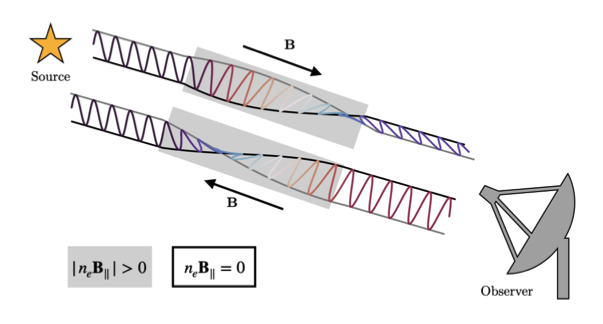
\includegraphics[width=0.8\linewidth]{Thesis_Template/Figures/Faraday_rot_diagram.png}
    \caption{A representation of Faraday Rotation as two electromagnetic waves travel from a source through two areas with oppositely orientated magnetic field (grey areas) towards the observer. The area with a magnetic field pointed towards the observer rotates the wave clockwise, whereas the area with a magnetic field pointed away from the observer rotates the wave anti-clockwise. Diagram from \cite{Emma_thesis}.}
    \label{fig:faraday rotation diagram}
\end{figure}

The FDF, $F(\phi)$ gives the intensity of polarised emission and polarisation angle as a function of FD and is defined by 

\begin{equation}
    P(\lambda^2) = \int_{\shortminus\infty}^{+\infty} F(\phi) e^{2i\phi\lambda^2}\space d\phi
    \label{eq: complex FDF}
\end{equation}

where $P(\lambda^2)$ is the complex fractional polarisation $P=\frac{Q+iU}{I}$. $Q+iU$ does not have a flat spectrum, so it will vary with frequency even in the absence of any Faraday rotation. Therefore $F(\phi)$ must also be a function of wavelength, $\lambda$. 

Equation \ref{eq: complex FDF} can be generalised using the weight function, also known as the sampling function, $W(\lambda^2)$ introduced in \cite{Brentjens_2005} to give the observed complex polarised emission:


\begin{equation}
    \Tilde{P}(\lambda^2) = W(\lambda^2)P(\lambda^2).
\end{equation}

The weight function is non zero at $\lambda^2$ where a measurement has been taken and zero elsewhere.

The Rotation Measure Spread Function (RMSF) is another useful concept which is used to represent the 'telescope beam' within Faraday space and is defined as

\begin{equation}
    %R(\phi) = K \overset{m}{\underset{i=1}{\sum}}W(\lambda_i^2)e^{-2i\phi(\lambda_i^2-\lambda_0^2)}
    R(\phi) = e^{i(\phi\lambda_c^2)}\frac{sin(\phi\Delta\lambda^2)}{\phi\Delta\lambda^2}
    \label{eq: RMSF}
\end{equation}


where $\Delta\lambda^2 = \lambda_2^2-\lambda_1^2$ is the width of $W(\lambda^2)$ (e.g. \cite{Dickey_2019}). The half power width of the RMSF represents the resolution in Faraday space and the sampling determines the sidelobe level. The FDF can also be deconvolved with the RMSF to remove the sidelobe response using the RMclean method described in \cite{Heald_2009}.

RM synthesis transforms the intensity and angle measured into Faraday depth space, with the discrete described by the following equation from \cite{Brentjens_2005}:

\begin{equation}
    \Tilde{F}(\phi) \approx K \overset{m}{\underset{i=1}{\sum}}\Tilde{P}(\lambda_i^2)e^{\shortminus2i\phi(\lambda_i^2-\lambda_0^2)}    \label{eq: discrete rm synth}
\end{equation}

where $\Tilde{F}(\phi)$ is the reconstructed Faraday dispersion function. More details on this process can be found in Chapter \ref{ch: RMsynth}.

\subsection{Rotation Measure Grids}

With a large number of polarised background sources for which the RM has been determined, the Galactic magnetic field structure at varying scales can be probed by making a map, or grid, of these measurement (\cite{Johnston_2015}). These grids can be used to statistically probe extended foreground sources, such as the Milky Way and Magellanic Clouds (e.g. \cite{Brown_2003}, \cite{1997A&A...322...98H}, \cite{1980ApJ...242...74S}, \cite{Haverkorn_2006}), on $\sim$ kpc scale, galaxy clusters and the cosmic web on $\sim$ Mpc scales (e.g. \cite{Akahori_2014}) as well as supernova remnants, pulsars and bubbles within the Milky Way and other nearly galaxies on kpc-pc scales (e.g. \cite{1984ApJ...287..295M}, \cite{Gaensler_2001}). 

%Observations of large scale field patterns and their superpositions supports the dynamo theory whereas the lack of these patterns suggests this is not the case, and that the field maybe had a primordial origin or is structured by gas flows.

\begin{figure}
    \centering
    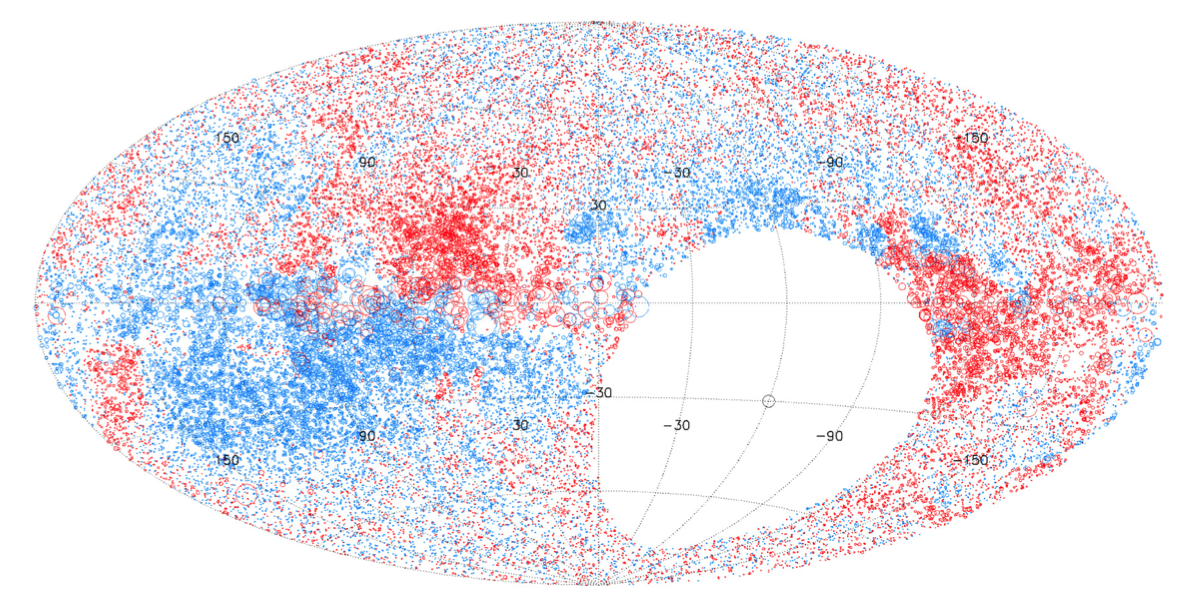
\includegraphics[width=\linewidth]{Thesis_Template/Figures/NVSS_RM_Grid.png}
    \caption{RM grid consisting of sources from NVSS, produced by \cite{Taylor_20009}, with red circles corresponding to positive rotation measure and blue to negative rotation measure and the size of the circle scales linearly with the magnitude of rotation measure.}
    \label{fig:Taylor RM grid}
\end{figure}

Large scale RM grids began to become a more widely used tool after \cite{Taylor_20009} re-analysed NRAO VLA Sky Survey (NVSS) data to calculate RM along the line of sight to 37,543 polarised sources. The RM grid has an average density on the sky of more than one RM per square degree, which was almost 2 orders of magnitude greater than any catalogue up to that point outside of the Galactic plane. Positive RM at each of the poles suggests that there is a sign reversal of the poloidal magnetic field across the Galactic plane. This catalogue has since been combined with other smaller RM catalogues by \cite{Oppermann_2012} which contains 41330 sources. \cite{Hutschenreuter_2020} then used a new inference algorithm to combine previous RM grids to produce a profile of the Faraday sky, which can be seen in Figure \ref{fig: Hutschenreuter 2020}.  This work was then updated to include almost all RM measurements available up to 2020 (\cite{Hutschenreuter_2022}). This catalogue 
consists of 55190 sources with a resolution of $1.3 
\times 10^{\shortminus2}$ square degrees. 
This resolution is twice that of previous endeavours. 
Much like the method used to produce the previous Hutschenreuter map, this map is produced using a Bayesian inference scheme. 

\begin{figure}
    \centering
    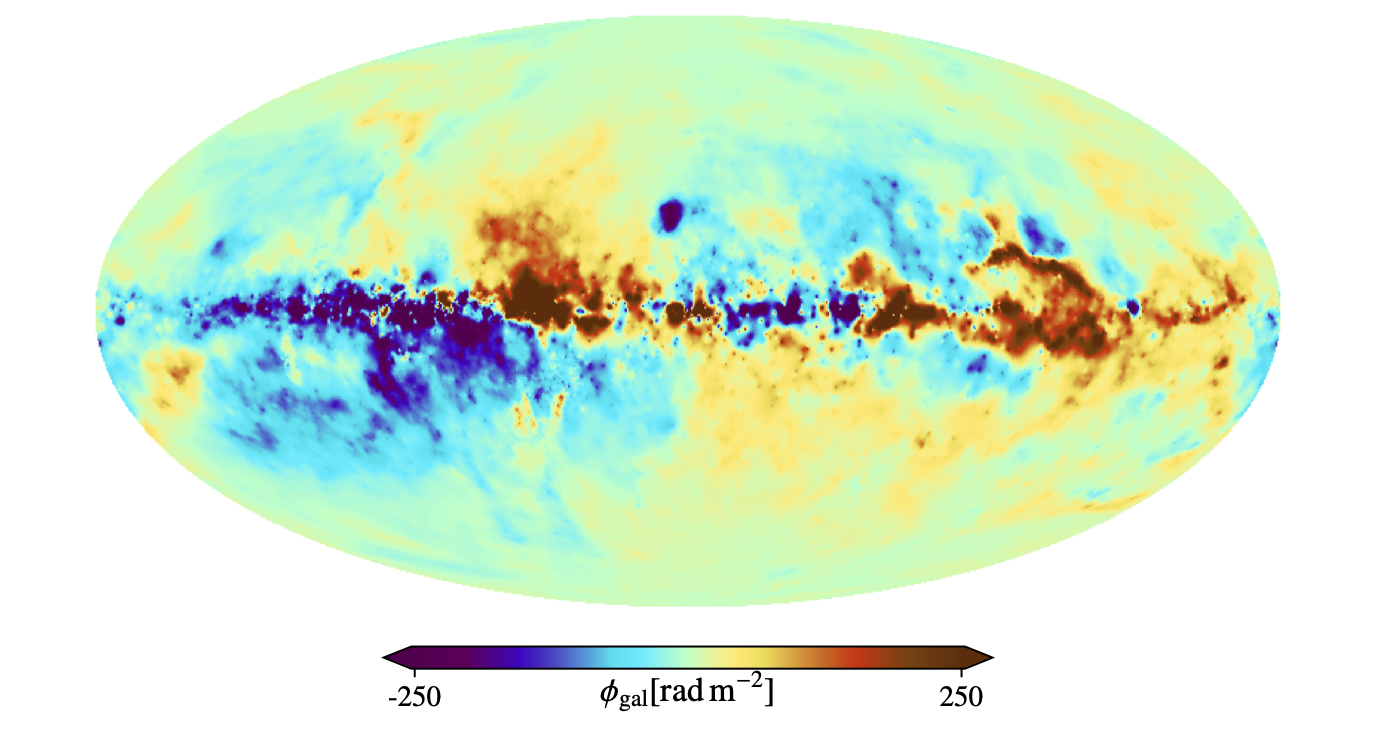
\includegraphics[width=\linewidth]{Thesis_Template/Figures/Hutschenreuter2020.png}
    \caption{The distribution of Galactic Faraday Rotation measure across the sky produced by \cite{Hutschenreuter_2020}, with the colour scale saturated at $\pm$ 250 rad$\,$m$^{\shortminus2}$}
    \label{fig: Hutschenreuter 2020}
\end{figure}

The most recent collection of RM has been compiled by \cite{vanEck_2023}. This catalogue was assembled to demonstrate the implementation of a proposed standard convention for RM catalogues, known as RMTable2023. This consolidates 55,819 RM from 42 published catalogues, making it the most comprehensive RM catalogue to date. These RM can be seen in Figure \ref{fig:van eck map}.

\begin{figure}
    \centering
    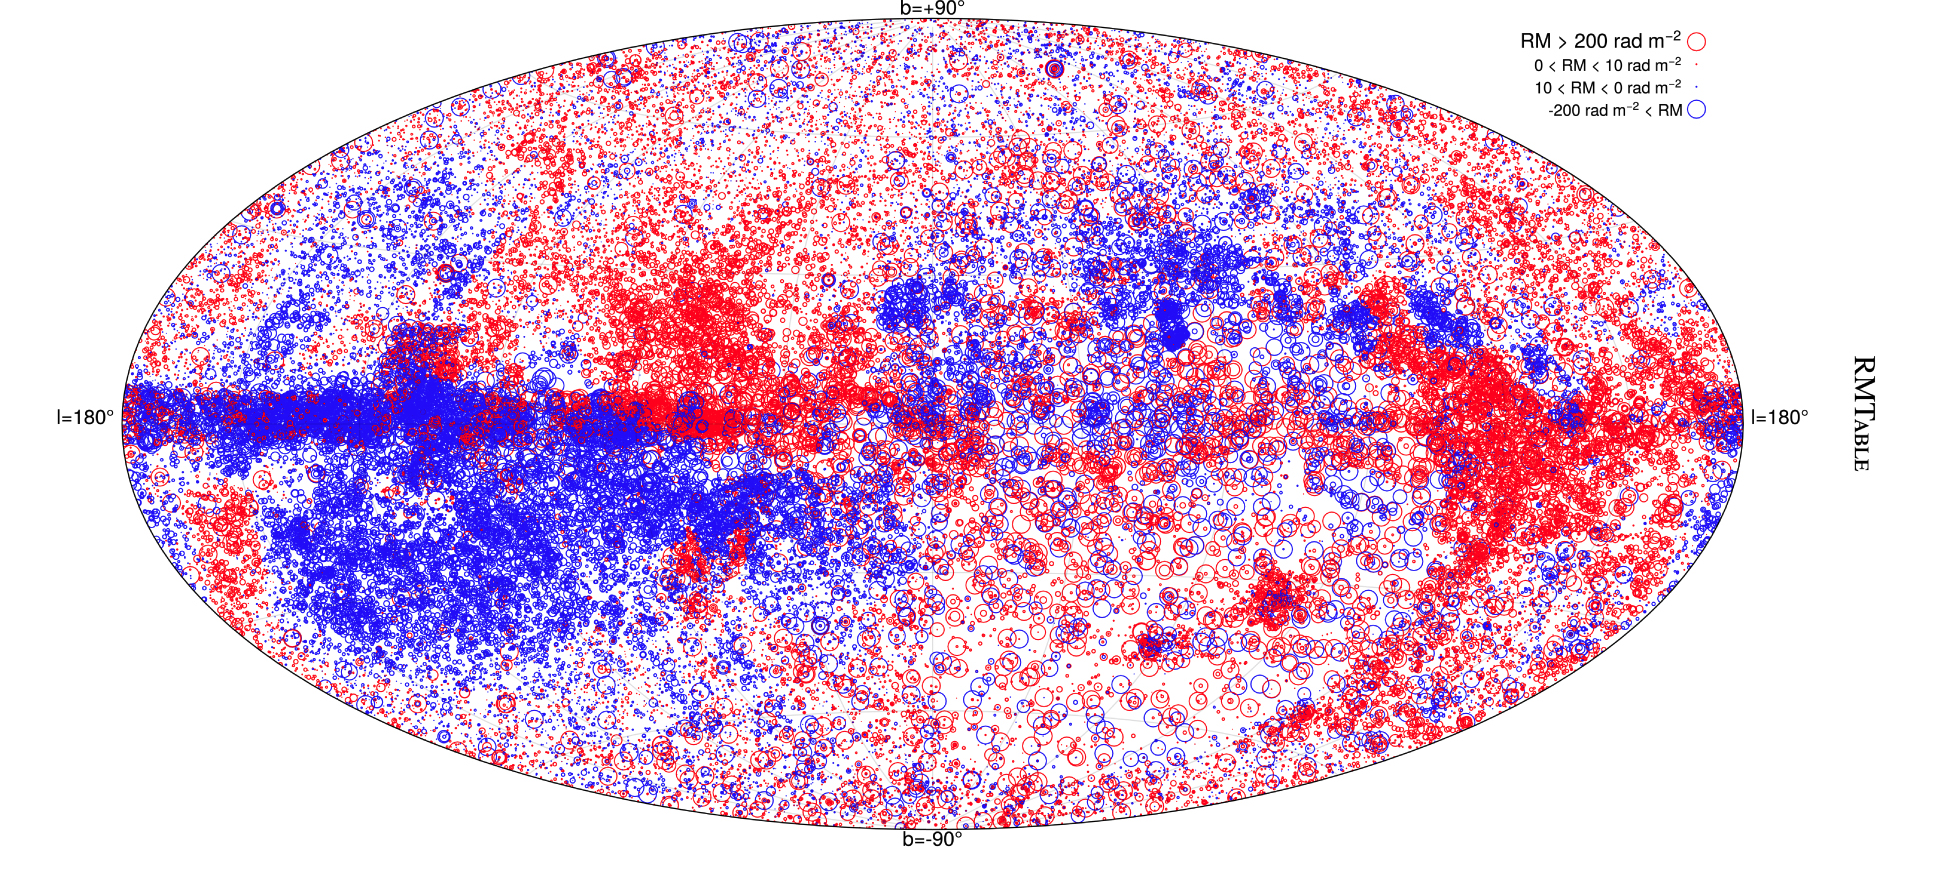
\includegraphics[width=\linewidth]{Thesis_Template/Figures/van eck map.png}
    \caption{Distribution of RM from \cite{vanEck_2023}. Each source is shown as a circle with diameter proportional to magnitude of RM, with the scale capped at 200 rad$\,$m$^{\shortminus2}$. Positive RMs are shown in red and negative in blue.}
    \label{fig:van eck map}
\end{figure}

These catalogues were lacking source density in the southern sky, however recent surveys such as S-PASS/ATCA (\cite{Schnitzeler_2019}) and the POlarised GLEAM Survey (POGS)
(\cite{POGS_2020}) have increased coverage in this region. 


Despite this progress, the average density over the entire sky is only 1.35 RM per square degree. This lack of density makes it difficult to detect and measure the small scale structure of the magnetic field. The southern hemisphere catalogues still have a much lower density than the NVSS region so the new all sky map does not have such an improved resolution as claimed. Ongoing projects such as SPICE-RACS (\cite{thomson2023rapidaskapcontinuumsurvey}) and POSSUM (\cite{POSSUM}) will further improve the southern density. 

Furthermore, it can be seen in Figure \ref{fig: Hutschenreuter 2020} that the structure appears to be more uniform at higher Galactic latitudes, and have a more complex structure along the Galactic plane. Higher resolution is needed to accurately map the rotation measure at low latitudes, as the average distance is much larger at low latitude so a higher density is required to accurately observed the structure in this region.  

\subsection{Faraday Depolarisation}

Bandwidth depolarisation occurs when Faraday rotation happens within an individual channel of bandwidth $\Delta\nu$ at wavelength $\lambda_0$. This depolarisation can be described with the equation

\begin{equation}
    p = p_0 |\sin(\Delta\chi)/(\Delta\chi)|
    \label{eq: bandwidth depolarisation}
\end{equation}

where 
\begin{equation}
   \Delta\chi = 2\lambda_0^2RM\Delta\nu/\nu_0.
   \label{eq: deltachi}
\end{equation}


This places a limit on the maximum detectable RM of $RM_{max} \simeq \sqrt{3}/\Delta\nu$. 

Faraday depolarisation is caused by differential Faraday rotation. Differential Faraday rotation describes the effect of polarised planes of radio waves from the far side of the emitting layer being more rotated than those emitted from the near closest side, due to them passing through a magneto-ionic medium, or Faraday screen. The same effect can occur perpendicular to the line of sight, which can be indistinguishable from the first case if the FDF is the same. If the distribution of the emitting layer is assumed to have a symmetric magnetic field strength and distribution of thermal electrons along the line of sight, the degree of reduction of the polarisation can be described by a similar equation to Equation \ref{eq: bandwidth depolarisation} where it varies periodically with wavelength

\begin{equation}
    p = p_0 |\sin(2 RM \lambda^2)/(2RM\lambda^2)|
    \label{eq: Faraday depolarisation}
\end{equation}

and as it depends on RM, depolarisation therefore also depends on coherence length, field strength and thermal electron density. These periodic changes means that there is complete depolarisation at certain wavelengths. If the distribution is not perfectly symmetric, as is most often the case, non-periodic fluctuations in the polarisation occur as wavelength increases therefore complete depolarisation is very rare in reality.

There are thought to be two possible locations for the Faraday rotating medium in which the differential Faraday rotation takes place: internal, within the emission region itself, or external, within the foreground. To attempt to distinguish between the two requires high-resolution, low-frequency observations so that the Faraday screen is resolved, as extent of depolarisation has been shown to increase with decreasing frequency and resolution (e.g. \cite{cygnus_A}).


\section{POSSUM}

The Polarization Sky Survey of the Universe's Magnetism (POSSUM) is a commensal project using the Australian Square Kilometre Array Pathfinder (ASKAP) radio telescope as it observes for the EMU and WALLABY projects. This project will produce a continuum polarisation survey of the southern sky with a sensitivity of 17 $\mu$Jy/beam in Stokes Q and U and 30 $\mu$Jy/beam in Stokes I at 20" resolution with the aim to create a catalogue of Faraday rotation measures of various radio sources, including but not limited to radio galaxies, supernova remnants and pulsar wind nebulae (\cite{POSSUM}). When complete, the survey will have covered 20, 600 square degrees of the Southern sky.

ASKAP is a high dynamic range wide field survey telescope in a radio-quiet area of the Western Australia outback. Each of its 36 antennas has a 12-m diameter and is fitted with a focal plane phased-array feed (PAF) system which increases the field of view to 30 square degree (\cite{ASKAP}). A PAF consists of 188 receivers and low-noise amplifiers and is mounted at the focal point of each antenna. They are used to synthesise a 6 x 6 grid of virtual feeds which cover the field of view where each virtual feed has a primary beam defined by the telescope diffraction limit, $\theta = 1.22\frac{\lambda}{D}$.




Upon completion, POSSUM will have created an RM grid containing roughly one million linearly polarised sources. This grid will allow for study of the the magnetic field on smaller scales than previously possible due to its order-of-magnitude decrease in RM uncertainties, with a median uncertainty of $\approx 1$ rad$\,$m$^{\shortminus2}$. The completed RM grid will be about 30 times more dense than the data used for the most recently produced RM grid \cite{Hutschenreuter_2020}. POSSUM also measures RM in over 288 frequency channels, whereas NVSS only measured over 2 channels. This increase in frequency range allows for greater accuracy when the rotation between the channels is greater than 90$^\circ$, which is key for rapidly varying RM at low latitudes.

\subsection{Imaging Pipeline}


ASKAP-POSSUM pipeline, maintained and run by the ASKAP observatory, conducts calibration and imaging and produces the data products such as images and data cubes. Swiftly after each observation is complete it is processed by the pipeline. After initial flagging, the unpolarised calibrator source PK1934-638 used to derive the bandpass, and then further flagging is applied to the target data after the bandpass solution is applied. Gain variations for each beam are then derived using a single amplitude and phase self calibration iteration. Images and Stokes spectral cubes are made and CLEANed independently per beam, stokes parameter and channel. The point spread functions (PSF) for each of the 36 beams are not identical due to sampling different spatial frequencies and different flagging so to combine the beams the smallest beam size for each channel is identified and then all beams are convolved to this beam size. The images from each beam are then linearly mosaicked, using full-Stokes models of the primary beam, to form a single image or data cube for that observation. The overlapping beams provide a near-uniform sensitivity across the field after this process. 

The standard image created has a 15 arcsecond resolution, but a high resolution image is also created which has a resolution of 9 arcseconds which gives four times as much detail as the standard image. This image is created reweighting the UV data with a uniform robustness, as opposed to the Briggs weighting used for the standard resolution image. The beam has a major and minor axis of 0.002 and a position angle of 77.05. Due to the new weighting, the high resolution image has almost twice the noise level as the standard image;  the high resolution image has a background noise level of $69 {\rm\, \mu Jy}$ where as the standard image only has a noise level of $38 {\rm\, \mu Jy}$.

Finally, the source finding algorithm Selavy is run on the standard Stokes I image to form a catalogue of sources, detailing their position and observed intensity. More details on this step are outlined in Section \ref{ch: sourcefinding}.

Another key part of this project is the science-ready processing pipeline, which contain the 1- and 3- dimensional polarimetry pipelines, which I have used to conduct the rotation measure synthesis. More information about these pipelines can be found in Sections \ref{POSSUM pipeline 1d} and \ref{3d pipeline}.

\subsection{Polarisation Leakage}

Polarisation leakage refers to the mixing of Stokes parameters observed by individual antennas of the interferometer, which is means that the nominal polarisation recorded by each antenna distorts the true polarisation. This distortion can be quantified by a Mueller matrix (e.g. \cite{2009_mueller}, \cite{gil2022polarized}). Most noticeably, emission from Stokes I can appear to 'leak' into the other parameters, as it is the parameter with the highest intensity. Polarisation can also leak from Q and U to I however as I component is much larger this has less effect. Leakage between Q and U is negligible in ASKAP (\cite{sault2015aces}). This phenomena is effectively independent of frequency.

During the imaging pipeline processing the UV data is corrected, using that assumption that the leakage is constant at the value measured from on-axis polarisation calibrators. This is referred to as the on-axis leakage correction. 

After the maps are made, the Q and U spectral cubes of each PAF beam are corrected for each component of the leakage that varies across the primary beam response in each PAF beam, This is referred to as the off-axis leakage correction. Leakage generally increases with distance from axis, so this is normally a larger correction than the on-axis correction. 

However, for early POSSUM observations which were validated and accepted before 5th October 2023, for which the field 1505-60 is one, the off-axis correction actually included the leakage at the beam centre, which means that in effect the on-axis correction is applied twice. This creates an artificial leakage equal and opposite to the original on-axis leakage and resulted in an leakage of typically around $1\%$ of Stokes I into Stokes Q and U. The leakage does not vary greatly with frequency so produces a RM component close to 0 in the FDF. This has now been fixed and the leakage is mostly less than 0.05$\%$.

The on-axis instrumental polarisation calibration for each beam is derived once every 24 hours using the primary calibrator PKS B1934-638 and models of the ASKAP primary beams are found using holographic measurements of the unresolved, unpolarised calibrator source PKS B0408-65 (\cite{POSSUM}). Holographic techniques use a Fourier transform to find the aperture field distribution from the diffraction pattern. This distribution can then be used to characterise the surface of the antenna to give the axial offsets of individual structural panels (\cite{hotan2016holographic}).

\subsection{POSSUM Pilot}

POSSUM has had two pilot phases of 100 hours of observing time each. The first phase covered 270 square degrees and overlapped with the first EMU pilot survey but with a different, higher, frequency range. The second pilot phase was designed to test the efficacy of the projects commensality with EMU, in frequency band 1 (800$\shortminus$1088 MHz), and WALLABY, in frequency band 2 (1296$\shortminus$1440 MHz). The full survey is currently ongoing. 

\cite{vanderwoude2024prototypefaradayrotationmeasure} analysed four fields from the pilot observations, including one Galactic field in the ASKAP low band, the results of which were the motivation for this work. 

The field that crossed the Galactic plane was found to have the lowest density of polarised sources of the fields investigated, with 20.2 RM per square degree, less than half that of the other fields that do not cross the Galactic plane. For this analysis, source finding was carried out by the ASKAP Observatory, who used the source finding software Selavy. Fewer sources were found in the Galactic field because Selavy works by finding islands above a threshold set by the local rms and in the plane this rms is set by the continuous band of Galactic nebulae rather than the expected thermal noise which is the case in the higher latitude fields. At low frequencies, below $\sim 100\,{\rm MHz}$, HII regions can be seen as discrete regions of absorption due to free-free absorption. This absorption leads to high opacity, depending on the line of sight between the observer and the HII region (\cite{free_free}). This problem of noise impacting the number of sources found is the key motivating factor for the work done for this dissertation.



The Galactic field has a line of sight through the Galactic plane, through the Scutum-Centaurus spiral arm of the Milky Way. It is noted that this field has much higher RM than the those in the other fields analysed in this paper, with a more complex structure.

\begin{figure}
    \centering
    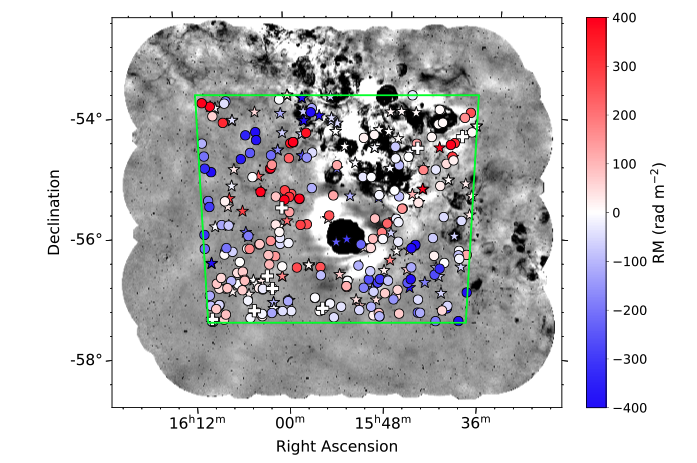
\includegraphics[width=0.9\linewidth]{Thesis_Template/Figures/Shannon_GL.png}
    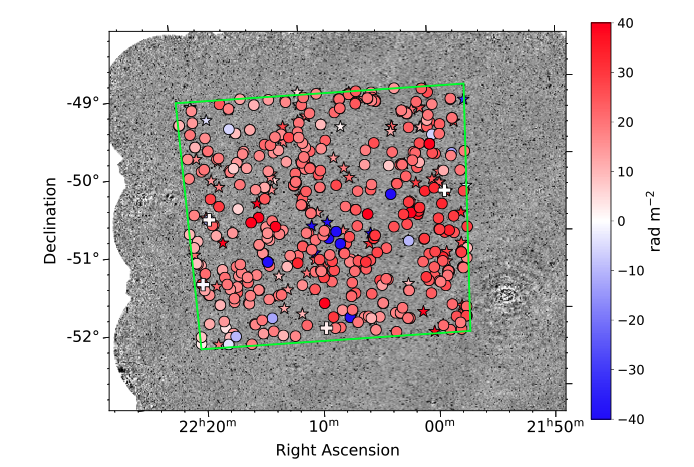
\includegraphics[width=0.9\linewidth]{Thesis_Template/Figures/Shannon_EC.png}
    \caption{Rotation measure grids from the POSSUM Pilot, produced by \cite{vanderwoude2024prototypefaradayrotationmeasure} with positive RM pictured in red and negative RM pictured in blue. The upper plot shows a field at low Galactic latitude crossing the Galactic plane, where the RM values vary between $\pm$400 rad$\,$m$^{\shortminus2}$ and the lower plot shows a field at high Galactic latitude, where the RM varies between $\pm$ 40 rad$\,$m$^{\shortminus2}$}
    \label{fig: Shannon's RM grids}
\end{figure}

There are two key features of Figure \ref{fig: Shannon's RM grids} that have motivated my own project: firstly, that the density of sources significantly decreases within the diffuse emission of the Galactic plane, and secondly, that there is significantly larger variation of the magnitude and sign of the RM on smaller scales, around 15 pc, within the Galactic field. The range of RM in the Galactic field is approximately 10 times that of the field with a higher Galactic latitude. As discussed previously, understanding the smaller scale structure of our Galaxy is vital to determine the origins of the magnetic field itself. In order to better understand the rapidly varying nature of the small scale structure of the magnetic field along the Galactic plane, it is paramount that the source density within the diffuse emission is improved.



\section{Summary and Overview}

In this chapter I have given an outline of the relevant background science to this dissertation, such as a description of astrophysical and Galactic magnetic fields, methods for detecting them and the motivation for the work carried out for this dissertation. In Chapter \ref{ch: sourcefinding} I describe the method used to increase source density within the Galactic plane and information on the source finding algorithm used. In the next section, Chapter \ref{ch: RMsynth}, I explain the POSSUM analysis pipeline and how it was used to create a rotation measure grid of the field EMU1505-60. I also present the structure function analysis carried out on the RM grid. In Chapter \ref{ch: Canals} I detail the additional investigation I carried out to investigate the polarisation of diffuse emission, using 3D RM synthesis to produce RM and polarised intensity maps of the field and analysis canal like structure detected within RM maps of other POSSUM fields.


\chapter{Finding New Sources in POSSUM Data}
\label{ch: sourcefinding}

The following chapter describes my investigation into a possible cause for the lack of rotation measure sources found within the diffuse emission of the Galactic plane and trialling a potential solution. This investigation was carried out on data produced by the POSSUM collaboration and the field chosen was EMU1505-60 (the range in right ascension and declination of this field are shown in Figure \ref{fig: validation_selavy}). This field was chosen as it crossed a significant amount of Galactic plane compared to the other fields available.

One possible reason for the low RM source density in along the Galactic plane is that the areas covered by diffuse emission that spreads across the Galactic plane is interpreted as regions of low signal to noise ratio by the source finder. This results in fewer overall sources being detected in these regions and thus fewer RM sources. Another possibility is that the sources within the Galactic plane are depolarised, so their RM is more difficult to detect. This research focuses on addressing the first reason and devising a method to reduce noise and increase the source density.

%pretty sure thats not quite right and that last sentence needs work! also i think this should be in the introduction


% Why it is useful
% How it is done

In order to complete any analysis of sources within radio interferometric data, the positions of these sources must be accurately found. Therefore reliable and accurate source finding methods are key to any sort of radio astronomy. As the capabilities of interferometers has  increased, the number of sources visible in images has also increased and for many years now a manual approach has been unfeasible. Therefore, a variety of different automated software packages have been developed over the last 60 years. The technique most used by these programs is based on the idea of fitting two-dimensional Gaussians to areas that have emission above a given threshold. This method extracts information about both the location and intensity each source. A catalogue of this information is then output as the result for a given image.

\section{Initial Source List}

As part of the ASKAP Observatory pipeline which is run on each POSSUM field prior to data release, a source list for the field was generated using the the source finding software Selavy (\cite{Selavy_Whiting_2012}). This found a total of 10881 components, which can be seen in Figure \ref{fig: validation_selavy}. These point sources are mostly radio galaxies, but there are other extended sources such as a pulsar wind nebula and multiple supernova remnants, most notably the supernova remnant MSH 15-22 (see Figure \ref{fig:sn remnant}) that have been detected as groups of point sources. 


\begin{sidewaysfigure}

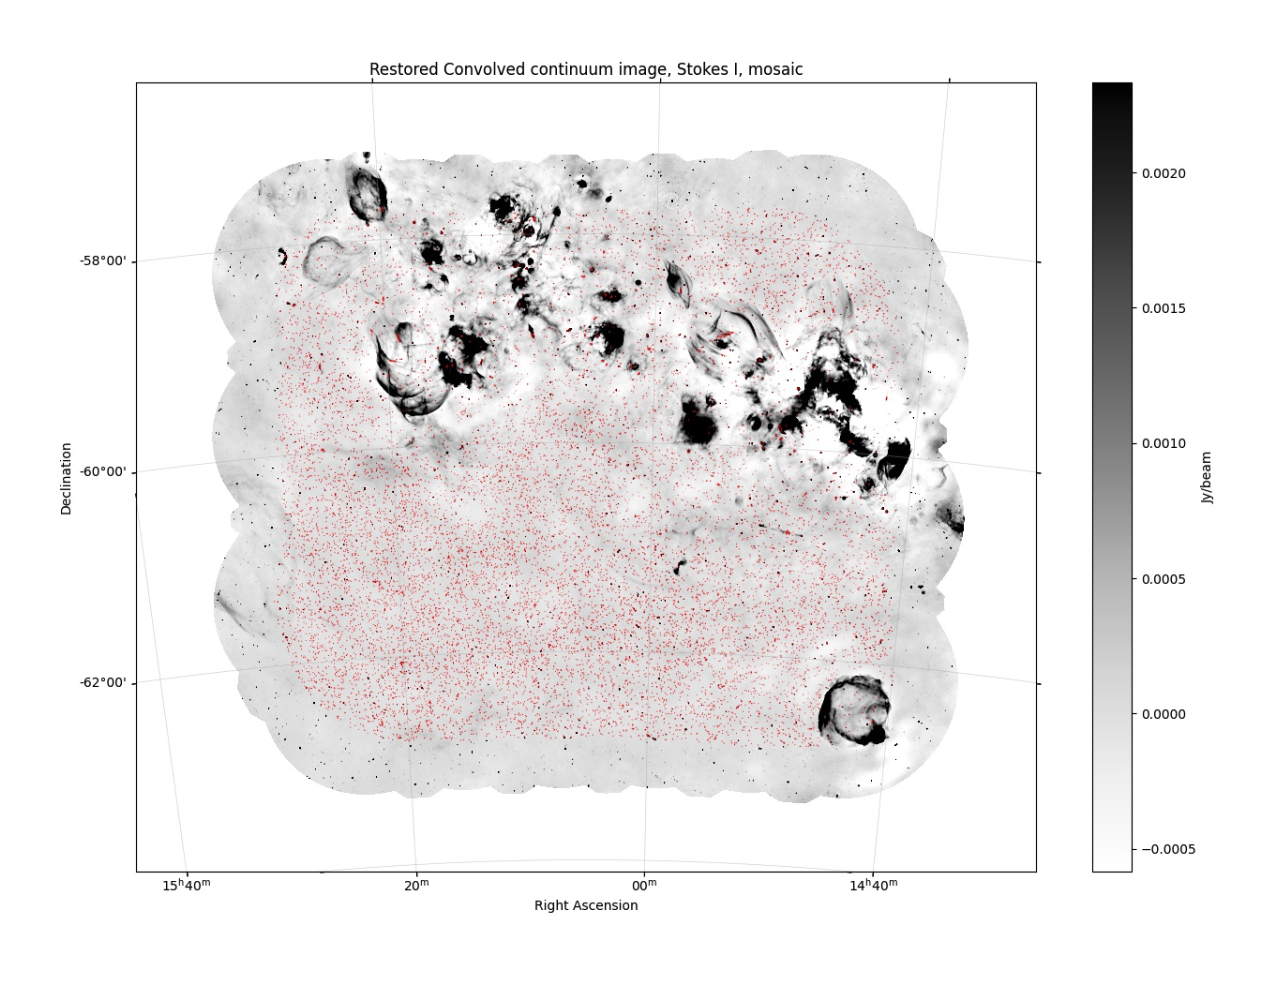
\includegraphics[width=0.8\linewidth]{Thesis_Template/Figures/validation_sourcefinder.png}
\caption[Source catalogue produced by ASKAP Observatory pipeline]{Source catalogue output by Selavy as part of ASKAP Observatory pipeline for field EMU1505-60, produced by \cite{validation}, with each point mapped as a red dot, and the intensity of the field image shown by the grey scale}
\label{fig: validation_selavy}
\end{sidewaysfigure}

\begin{figure}
    \centering
    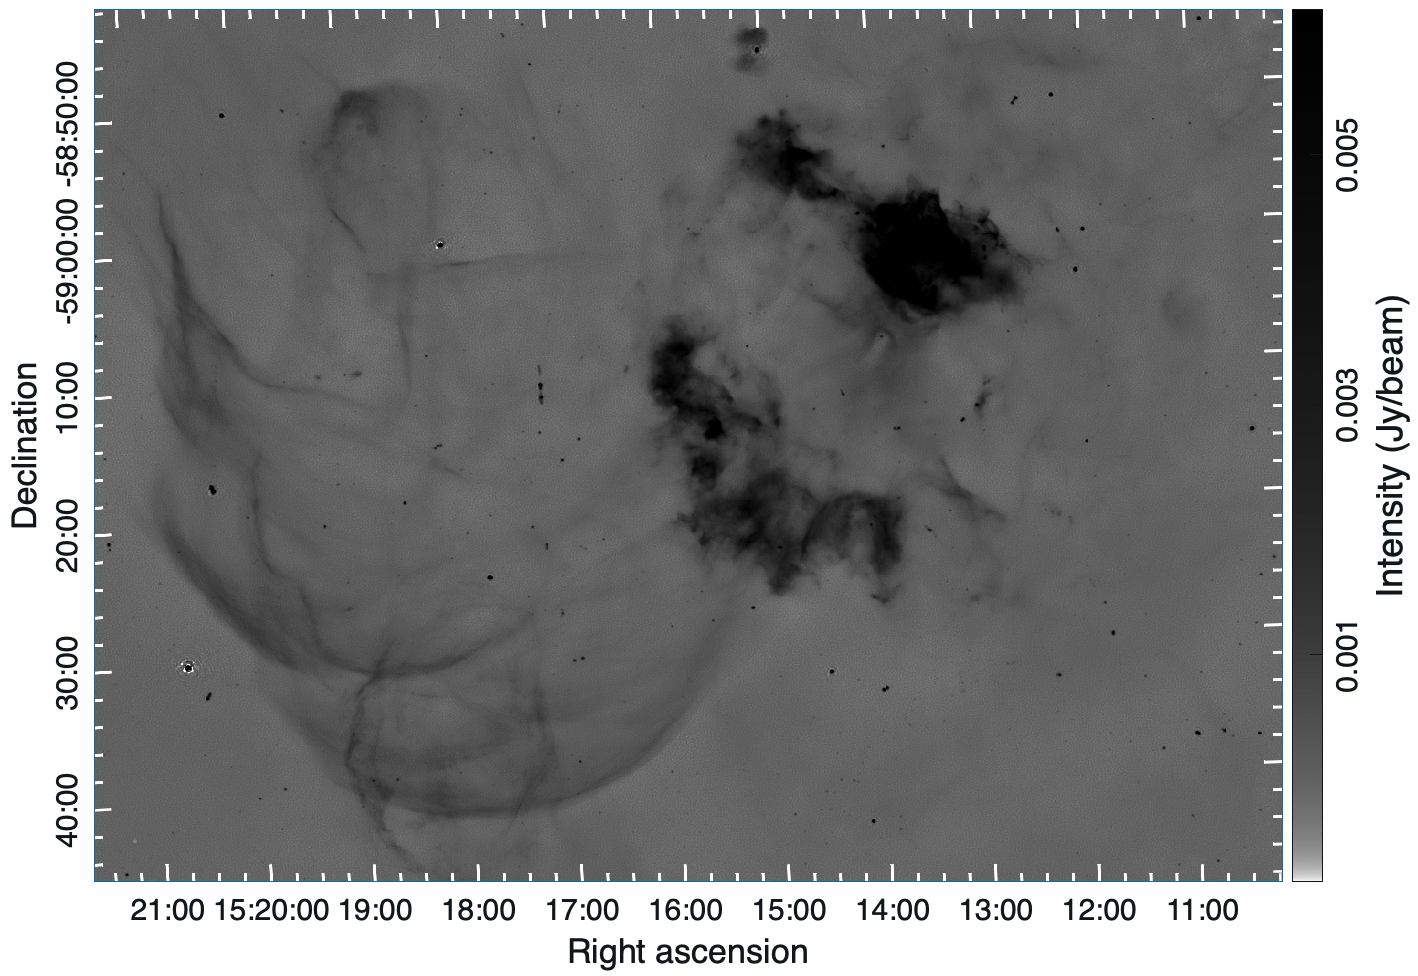
\includegraphics[width=\linewidth]{Thesis_Template/Figures/EMU_1505-60_hi.fits-image-2025-04-24-17-38-58.png}
    \caption[Supernova remnant MSH 15-22]{Zoomed in image of the supernova remnant MSH 15-22 in the hires image using an asinh greyscale which runs from linear near zero and logarithmic for bright emission to highlight all the structure within the nebula}
    \label{fig:sn remnant}
\end{figure}

Selavy is an implementation of the Duchamp source finder (\cite{Duchamp_Whiting_2012}) with additional features designed for ASKAP. Duchamp was initially developed to process three-dimensional spectral line cubes, but could also handle one and two dimensional data sets. 

Much like in Figure \ref{fig: Shannon's RM grids}, it is apparent in Figure \ref{fig: validation_selavy} that there is a distinct lack of sources found along the Galactic plane. There is a stark difference in source density between on and off the Galactic plane, which is demonstrated by Figure \ref{fig:source density in selavy}. The two boxes show the sources within that region with the upper box located on the Galactic plane and the lower box located in an area without diffuse emission. The source density within the diffuse emission is 78 sources per square degree whereas without any diffuse emission the source density is nearly five times greater at 387 sources per square degree. Some of the sources within this area may however be peaks within the nebula of the supernova remnant within this field, which can be seen in greater detail in Figure \ref{fig:sn remnant}.

\begin{figure}
    \centering
    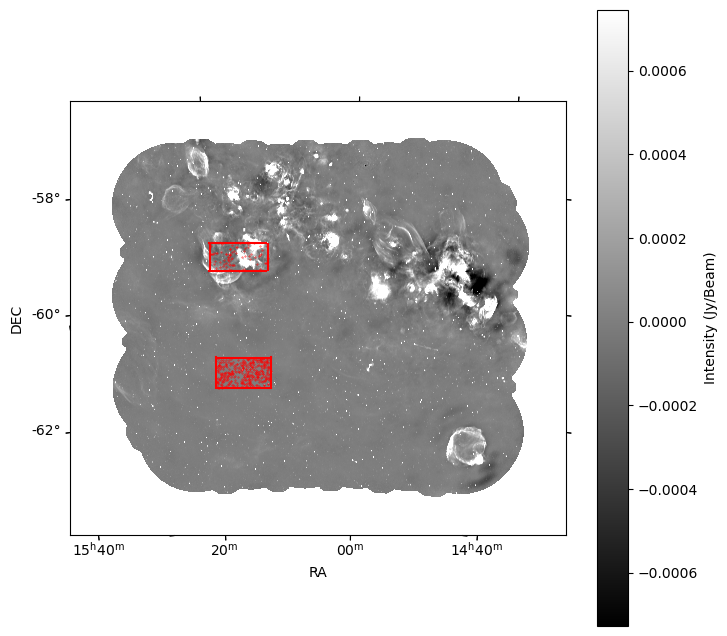
\includegraphics[width=1\linewidth]{Thesis_Template//Figures/source_density_comparison.png}
    \caption[Source density comparison between on and off the Galactic Plane]{Source Density Comparison of Selavy catalogue between on and off the Galactic Plane}
    \label{fig:source density in selavy}
\end{figure}

The vast majority of the radio sources found by Selavy are extragalactic so we would expect a near-uniform density of sources across all Galactic latitudes, except for minor fluctuations due to the structure of the cosmic web and rare instances of sufficiently compact Galactic sources, such as radio stars, pulsars or peaks in nebulae. Therefore, an explanation is required for this disparity.


\section{Re-Processing} 

In order to reduce the noise, so that more sources can be detected within the diffuse emission, I have reprocessed the image given to the source finder in order to improve the visibility of the sources by removing as much diffuse emission as possible.

When I began this process, I decided to use the higher resolution image produced by EMU. This was the first step in suppressing the noise created in the image by the diffuse emission. When comparing the standard resolution image, Figure \ref{fig: low_res}, with the high resolution image, Figure \ref{fig: high res}, it is clear that the apparent brightness of the diffuse emission is reduced. Another key difference is that the negative 'bowl' artefacts, which are caused by missing short spacings are reduced as the uniform weighting gives higher weight to the short baselines, thus picking up extended structure. One disadvantage however is that the noise is increased and there stippled noise pattern which is not present in the low resolution image. Moreover, after CLEANing to a fixed threshold, extended nebulae retain much flux density within the dirty map and as it has not been deconvolved and is only detected on a few short baselines, large sidelobes remain.

\begin{figure}
    \centering
    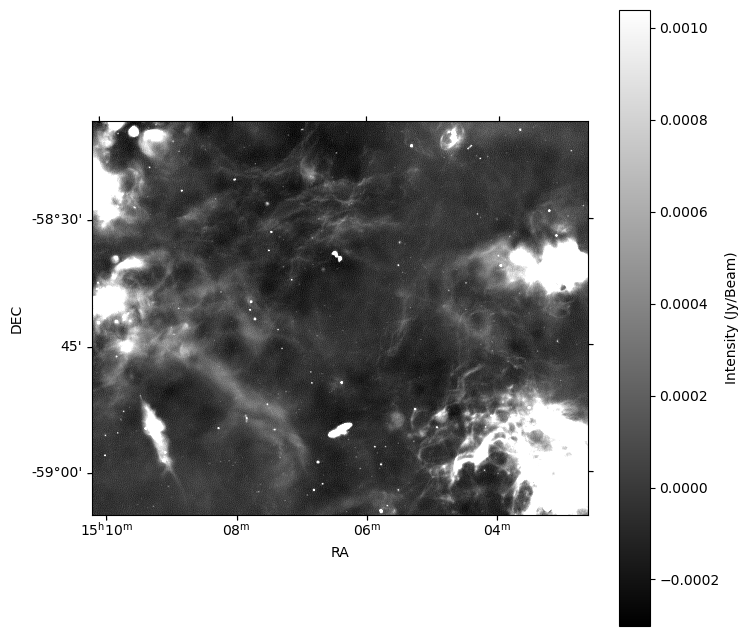
\includegraphics[width=1\linewidth]{Thesis_Template/Figures/hires_crop.png}
    \caption[Cropped high resolution image of the EMU1505-60 field.]{Cropped high resolution image of the EMU1505-60 field, highlighting the difference in noise between this and the low resolution image.}
    \label{fig: high res}
\end{figure}


\begin{figure}

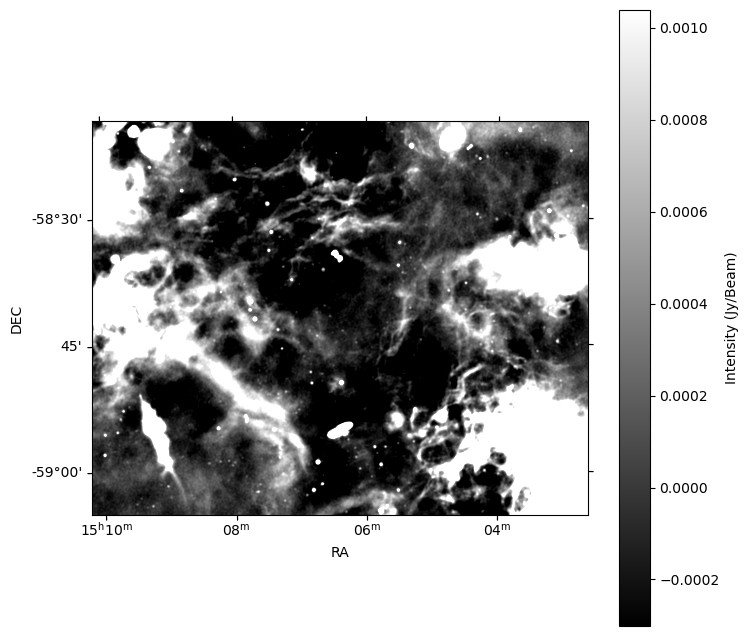
\includegraphics[width=1\linewidth]{Thesis_Template/Figures/lores_crop.png}
\caption[Low resolution, or standard, image of field EMU1505-60.]{Low resolution, or standard, image of field EMU1505-60, highlighting the difference in noise between this and the high resolution image.}
\label{fig: low_res}
\end{figure}


The region around the edge of each individual POSSUM field has high noise due to the primary beam correction. To remove this, I created a subsection of the image, and subsequently each Stokes parameter cube, using AIPS. The size of this section was chosen to have dimensions of $8192{\rm \, x\,}8192$ pixels because a power-of-two size will speed up the Fourier transform performed for RM synthesis.


\subsection{Masking}

In order to suppress the diffuse galactic emission I used the AIPS program NINER to apply a peak finding filter. This served to highlight the point sources and reduced the apparent brightness of the large scale galactic structure. NINER works by convolving a 3 x 3 matrix with each cell of an image and its 8 nearest cells. 

The matrix used is shown below.


\begin{equation}
    \begin{bmatrix}

    -1 & -1 & -1\\
    -1 & 8 & -1\\
    -1&-1&-1
    
    \end{bmatrix}
    \label{eq: msk2}
\end{equation}

\noindent This process successfully suppressed the diffuse emission, leaving behind a field dominated by point sources. The variation in the noise background can be seen in Figure \ref{fig: niner} to be greatly reduced, compared to both Figure \ref{fig: high res} and Figure \ref{fig: low_res}. This does however greatly increase the noise, as this image has a background rms of $200 \,\mu{\rm Jy}$, which is almost six times that of the standard image. This affects the flux measured for each source. The next step was to use a source finding algorithm to locate these sources.

% ppp add figure of niner result

\begin{figure}
    \centering
    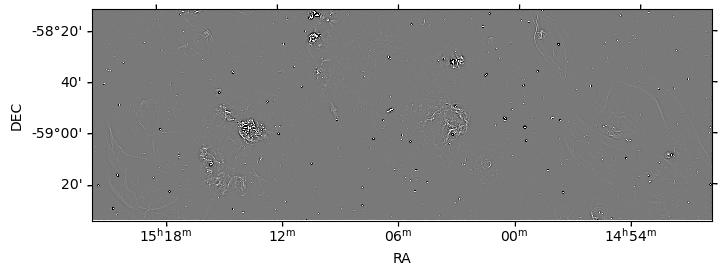
\includegraphics[width=1\linewidth]{Thesis_Template/Figures/niner.png}
    \caption[NINER output]{A zoom in of the NINER output image showing the point sources highlighted by this convolution process}
    \label{fig: niner}
\end{figure}



\section{Source Finding Algorithms}

There are many source finding algorithms available, each with their own strengths and weaknesses, so a decision had to be made as to which one to use. The source finder used in the ASKAP Observatory pipeline is Selavy. This source finding algorithm works by grouping pixels in an image that are three times the root-mean-square (rms) of the image, and then fitting a Gaussian to peaks within the islands, with only peaks with an intensity of above five times the rms being counted as sources. The rms is found by calculating the median absolute deviation from the median (MADFM) and the same value is applied across the entire image. MADFM was chosen as a proxy for standard deviation due to its robustness against bright pixels which would otherwise contribute to the background noise calculation (\cite{Duchamp_Whiting_2012}). 

To help find which would be the most suitable tool, I referred to the results of The ASKAP/EMU Source Finding Data Challenge (\cite{data_challenge}). This was an investigation carried out by POSSUM's sister survey EMU with the aim of assessing the various merits and downfalls of many source finding algorithms currently available. The challenge involved creating three artificial source lists and images with source brightness and quantity of extended sources which many source finders, including Selavy, were then run on. The results from each source finder were then compared by quantifying their accuracy and identifying their limitations. 

The Python Blob Detector and Source Finder (PyBDSF)\footnote{PyBDSF can be accessed at https://github.com/lofar-astron/PyBDSF/tree/master} showed high completeness whilst also maintaining high reliability in the fainter, psuedo-realistic catalogue they had generated. Selavy, however, showed a very low reliability in this challenge. Furthermore, Selavy would be difficult to implement as it is currently only available as part of the data processing pipeline, whereas PyBDSF could be installed separately. Therefore, I made the decision to use PyBDSF instead.

PyBDSF (\cite{PyBDSF}) works by first calculating the background rms and mean images, which is done by using a box of a sensible size, which was chosen to be 819x819 pixels, and calculating the mean and standard deviation within the box at multiple places across the image with a step size of 273 pixels. Outliers are then excluded and the process is repeated iteratively until a constant value is reached. A threshold between background and source is set and then islands made of adjacent point sources are found. The threshold can be chosen to be either hard thresholding or using the False Detection rate method, or if it is not set, the program chooses the most appropriate based on the ratio of expected false pixels to true pixels. The hard thresholding was chosen by the program, which uses a 5-sigma for the pixel threshold and 3-sigma for the island boundaries. These islands are then simultaneously fit with multiple Gaussians with the number of Gaussians fit is determined by the number of distinct peaks, with a peak being defined by having a negative gradient in all eight directions. Then, those Gaussians are grouped into discrete sources. Groups within these islands are considered a discrete source if they are obviously distinct on the image. This distinction is calculated as if the difference between the peak of the lower Gaussian and the minimum value directly between the centre of each Gaussian is less than the product of the island threshold and the island rms and the distance between peak centres is less than half the sum of their full width half maximum value along the line joining them then they are categorised as the same source. The location and size of that source is then found by moment analysis %do I need to explain moment analysis?
and the flux found by the sum of the Gaussians within the source.

As the final step towards producing the improved source list, I ran PyBDSF on the processed image. This then produced a catalogue of sources, with location and intensity information. The sources found can be seen in Figure \ref{fig:pybdsf sourcelist}. This is another benefit of PyBDSF as it produces a list of sources and Gaussian components, for which I used the list of sources for further analysis, whereas Selavy only produces a list of Gaussian components which then have to be later grouped into sources by the user.

\begin{figure}
    \centering
    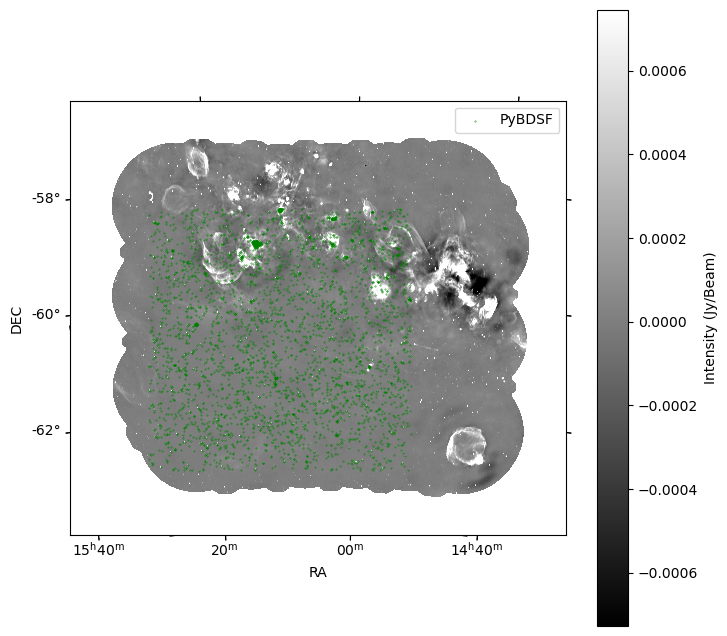
\includegraphics[width=\linewidth]{Thesis_Template/Figures/pybdsf_catalogue_legend.png}
    \caption[All sources found by PyBDSF]{All sources found by the PyBDSF source finding algorithm when run on the reprocessed image}
    \label{fig:pybdsf sourcelist}
\end{figure}


\section{Comparison of Source Catalogues}

In order to find if an improvement had been made by using the method outlined here, I conducted some comparisons between the original catalogue produced by Selavy during the observatory pipeline processing and the PyBDSF catalogue.

The first comparison I made was to see whether there has been a net increase in sources within the field processed with this method. I found that the source list created by PyBDSF after the reprocessing found fewer sources than the same subsection in Selavy.  However, this is to be expected, as the high resolution image has higher noise than the low resolution used for initial source finding, and moreover the implementation of NINER further increased the noise level throughout the image. The increase in noise from this process has affected the flux found by the source finder. By picking three point sources and comparing the flux measured by for that source by both Selavy and PyBDSF I have found that there is on average a 32$\%$ increase in flux from the Selavy to the PyBDSF catalogue.

To make a useful comparison I have focused my comparative efforts on the region shown in Figure \ref{fig: comparison_blank}. This region was chosen to cover as much of the diffuse emission as possible without including excess regions of clear sky so that the difference can be clearly measured.

\begin{figure}

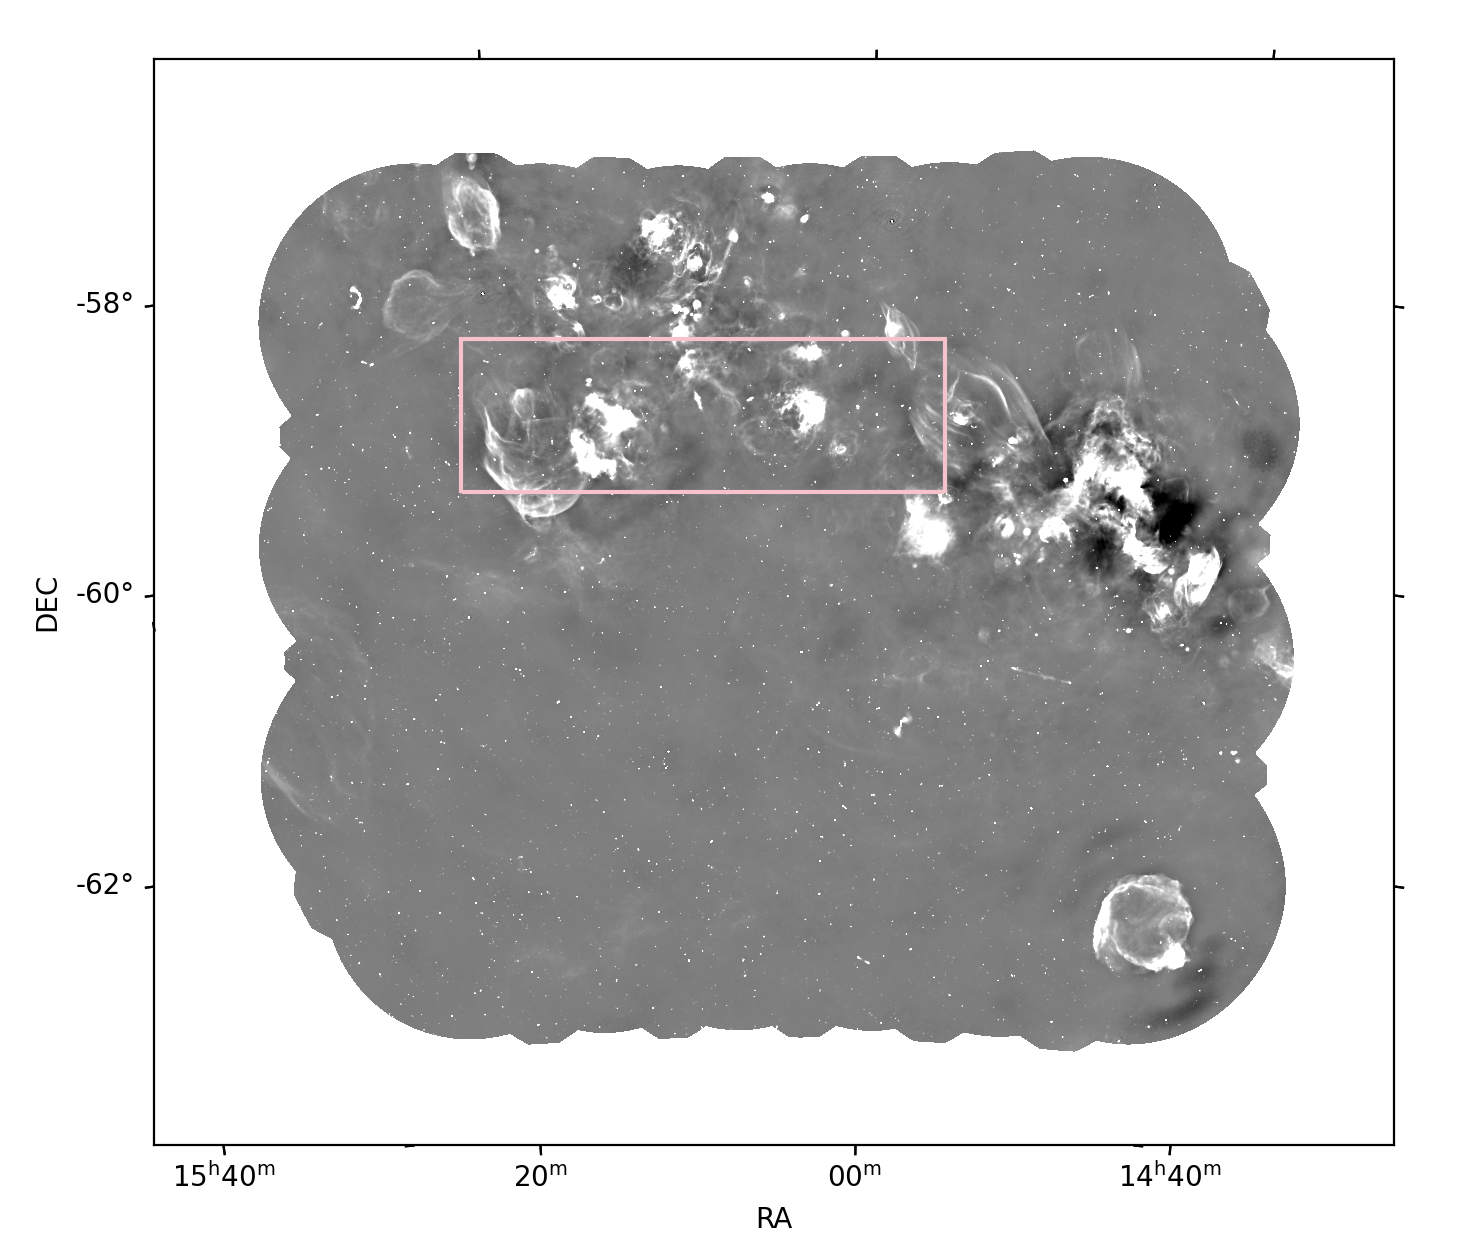
\includegraphics[width=0.9\linewidth]{Thesis_Template/Figures/comparison region.png}
\caption[Region chosen for source list comparison]{\small Region within field EMU1505-60 chosen for comparison between the source list produced for this project and the source list produced as part of the observatory pipeline for the field.}
\label{fig: comparison_blank}
\end{figure}

Within this comparison region, the Selavy catalogue contains 650 sources, whereas the PyBDSF catalogue contains 854 sources. This shows a significant increase in sources detected within the Galactic plane.

I then assessed whether the sources were aligned between the two catalogues. To do this, I converted the position from Right Ascension and Declination into Cartesian coordinates for each source in the comparison region. I then calculated the separation between each pair of sources between the catalogues. I considered each pair of sources that are within 5 arcseconds of each other to be the same source. This separation was estimated manually to be a suitable estimation to distinguish sources. By pairing the sources in this way I found that there were sources from both catalogues which did not appear to have a match by this method. There were 509 sources that were found by PyBDSF and not Selavy, which can be seen in Figure \ref{fig: pybdsf not match}, and 345 sources that were found by Selavy but not PyBDSF, which can be seen in Figure \ref{fig: selavy not match}. The sources that were not found by PyBDSF in this region are mainly within areas of the comparison region that do not have much diffuse emission, and the opposite is true for the sources not found in the Selavy catalogue. This suggests that the method culminating in the PyBDSF source catalogue has successfully increased source finding within the diffuse emission of the Galactic plane.

\begin{figure}
    \centering
    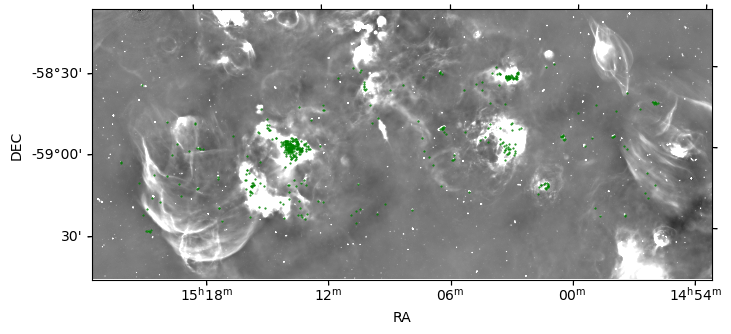
\includegraphics[width=\linewidth]{Thesis_Template/Figures/Py match.png}
    \caption[PyBDSF only sources]{Sources in the PyBDSF catalogue that were not within 5 arcseconds of a source in the Selavy catalogue}
    \label{fig: pybdsf not match}
\end{figure}

\begin{figure}
    \centering
    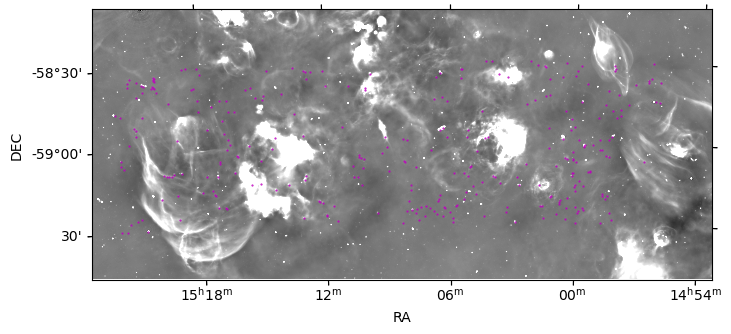
\includegraphics[width=\linewidth]{Thesis_Template/Figures/sel match.png}
    \caption[Selavy only sources]{Sources in the Selavy catalogue that were not within 5 arcseconds of a source in the PyBDSF catalogue}
    \label{fig: selavy not match}
\end{figure}

I also calculated the source density both on and off the Galactic plane in the same regions used for this calculation on the Selavy catalogue. This showed great improvement in source density for the region within the diffuse emission, with a density of 249 sources per square degree. This is over a 200$\%$ increase from the Selavy catalogue. There was, however, a decrease in source density off the Galactic plane, with a source density of 101 sources per square degree.

It is also worth noting that there is an over-density of PyBDSF sources in the bright region of the supernova remnant MSH15-22 and in the nebula at RA 15:03 and Dec -58:50. The source finder has mistaken bright emission peaks within the structure of the nebula for extragalactic sources. How the sources have been assigned to this nebula's structure can be seen in finer detail in Figure \ref{fig: snr sources}. Cases where sources are just peaks in brightness within the diffuse emission have been identified and removed from the catalogue via manual inspection.

\begin{figure}
    \centering
    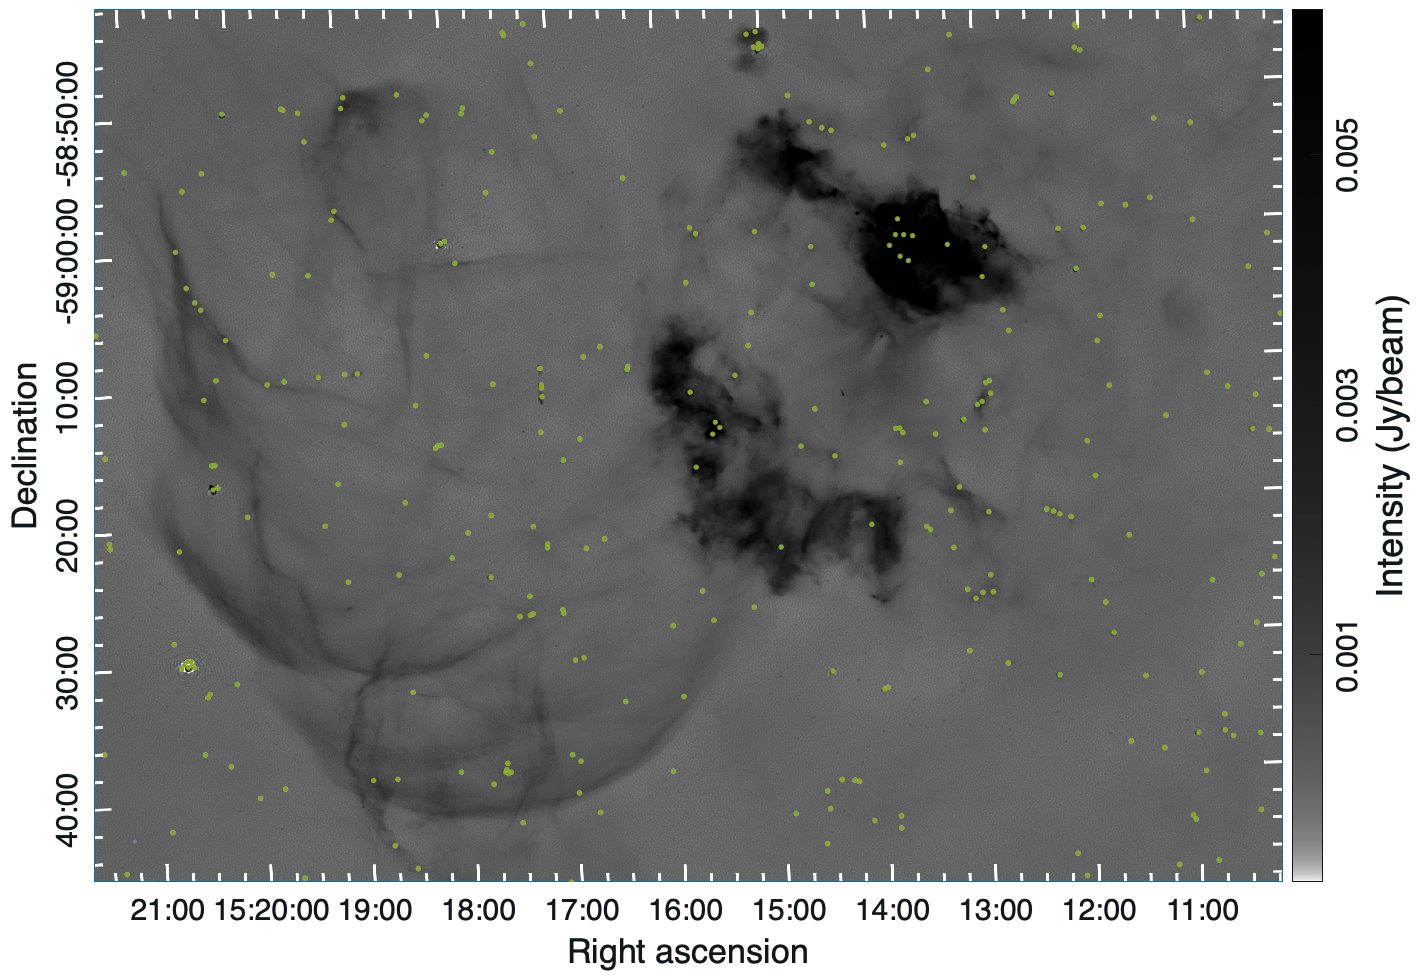
\includegraphics[width=\linewidth]{Thesis_Template/Figures/EMU_1505-60_hi.fits-image-2025-04-24-17-41-48.png}
    \caption{The supernova remnant MSH 15-22 with the 'sources' identified by PyBDSF}
    \label{fig: snr sources}
\end{figure}

\begin{figure}
    \centering
    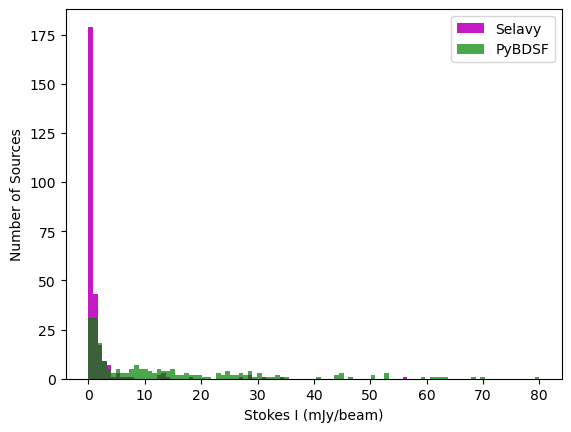
\includegraphics[width=\linewidth]{Thesis_Template/Figures/unmatched histogram.png}
    \caption[Histogram of flux densities for both source finding algorithms]{Histogram of flux densities for both source finding algorithms, with nebulae brightness peaks removed}
    \label{fig: unmatched histogram}
\end{figure}

Another point of interest, demonstrated in Figure \ref{fig: unmatched histogram}, is that the Selavy catalogue includes significantly more fainter sources, whereas the PyBDSF catalogue has found fewer faint sources but more sources. This histogram excludes the peaks in the brightness of the diffuse emission of the nebulae.

These results demonstrate that the diffuse emission is being interpreted as noise by the source finding algorithm, as convolving the image to smooth the image over the 3 x 3 matrix to highlight point sources has been successful in producing more sources within the Galactic plane. However, this convolution decreases source detection within areas without diffuse emission. This is because the gradient mask highlights sources with a large gradient, which highlights bright sources, but suppresses fainter sources which makes them less visible than they would normally be visible in areas with low noise or no diffuse emission. This means that convolution alone is not the optimal method for source finding over all fields and a combination between the initial source finding and this method should be employed.

These additional sources detected within the Galactic plane can then be used to conduct RM synthesis and thus find more RM within the Galactic plane, which will allow insight into the magnetic field of this rapidly varying region of the Milky Way. The next chapter details my implementation of the POSSUM polarimetry analysis pipeline to perform RM synthesis and the results it yielded.
\chapter{Probing the Small Scale Structure of Galactic Magnetic field}
%title tbd
\label{ch: RMsynth}

This chapter describes the work additional to the source finding that I have carried out in order to be able to run the 1-dimensional polarimetry pipeline on the data cube EMU1505-60, and then details the running of the pipeline's processes. When complete, the POSSUM science ready processing pipeline will conduct all the steps discussed in this chapter as well as making a correction for the ionospheric Faraday rotation and mosaic together adjacent fields of observation. As I am only processing one observation field, the ionospheric Faraday rotation is a few rad$\,$m$^{\shortminus2}$ and is constant across the field, so it would not affect the results of the structure function analysis detailed within this chapter. 

\section{Pre-Pipeline Processing}

\subsection{Convolution}

Before I ran the pipeline on the Stokes cubes I smoothed the I, Q and U cubes to a common resolution across all channels. This means that further analysis which is affected by resolution is easier to carry out. The Stokes data cubes all have 288 channels representing differing frequencies within the observation band. Each data cube was resampled to get three pixels across the final beam size and all maps were convolved using the CONVL task within AIPS. The cubes were then remade using the MCUBE task.

\subsection{Noise Profile}

My next step was to find the background noise of the image so that the I could accurately assign a weighting to each frequency channel to favour the least noisy channels. To do this, I first used AIPS to find the coordinates of five boxes which I made to contain as few sources as possible by selecting boxes manually within predominantly empty regions of the observed field. These boxes are shown in Figure \ref{fig: background noise boxes}.

\begin{figure}
    \centering
    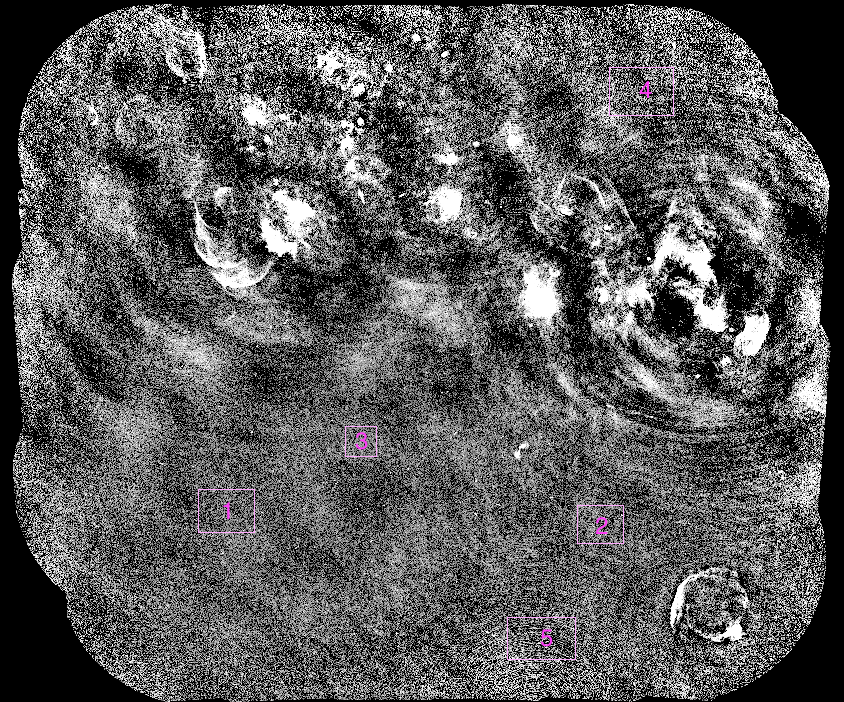
\includegraphics[width=0.9\linewidth]{Thesis_Template/Figures/Boxes for noise calculation image.png}
    \caption{Boxes chosen for background noise calculations}
    \label{fig: background noise boxes}
\end{figure}

I created smaller cubes of all frequency channels for each box, combined the boxes by stacking them into a single matrix and found the standard deviation of each frequency channel across all five boxes, which was very low between the different noise backgrounds ($<0.0004$). These are the values used in the pipeline for the weighting of the frequency channels.


\section{POSSUM Polarimetry Pipeline}
\label{POSSUM pipeline 1d}
The POSSUM polarimetry pipeline is the pipeline that will be applied to all the POSSUM fields in order to achieve one of the collaboration's core science case of producing an RM grid that covers the entire southern sky (\cite{POSSUM}). It mainly uses software from the RM-tools package created by \cite{RMtools} \footnote{RM-tools can be accessed at https://github.com/CIRADA-Tools/RM-Tools/tree/master}. This pipeline currently has two main routes: the 1-dimensional pipeline and the 3-dimensional pipeline. 


The 1D pipeline produces Faraday rotation measurements for sources in the predefined catalogue. From this pipeline I used eight steps: read sourcelist, extract spectra, diffuse subtraction, save spectra, rm synth 1D, clean catalog, write catalog and save FDFs.

The first step, read sourcelist, takes the output catalogue created by the source finding algorithm in the form of a fits file and turns it into an astropy table of dictionaries for each source. As the source finder used by ASKAP is Selavy, the pipeline was written to accommodate the format of the Selavy output catalogue. As I instead used PyBDSF as the source finder, I needed to change the names of the variables and conversion factors in order to account for the difference in input. Apart from this step, I ran each step as it had been written, my only input being selecting options and specifying input parameters.

The next step extracts the Stoke I, Q and U spectrum for each source in the source list and the median spectra for the diffuse emission surrounding the source. This is done by taking the mean pixel intensity for each source and the median and noise of the annulus around the source, with the inner and outer radii of the annulus given in the configuration file. The mean intensity is calculated by finding the sum of a 3x3 and 5x5 pixel window centred on the nearest listed source, in order to capture the slightly the off-peak polarisation and finally the sum is normalised using the synthesised Gaussian beam model. This method was found to be an improvement on the method of using the peak pixel as it is less sensitive to variations of the true source position within the peak pixel. The noise of the annulus is determined by applying an annulus shaped mask at each frequency for the source and taking the standard deviation. The annulus chosen had an inner radius of 35'' and an outer radius of 109''. This size means that it is possible that other sources could be in it, so this method of averaging over all frequency bands helps to negate their influence on the noise. The pipeline stores these as a dictionary. Any sources that are too close to the image edge are noted in the log file and their spectra assigned zero values. This was the case for 118 of the 3860 sources found by the source finding routine. The next step, diffuse subtraction, subtracts the median, from the annulus, from each source spectrum calculated in the previous step. These spectra are saved, so that they can be used again without re-extraction. This is useful because the extract spectra step takes over an hour to complete.

The next step is rotation measure synthesis, which for the one dimensional pipeline performs RM synthesis along single lines of sight using RM-tools. 
This routine uses a discrete Fourier transform to calculate the Faraday dispersion function (FDF) using the equation to transform the spectra from frequency space to Faraday depth space. In order to achieve RM synthesis a FDF is fit to each spectrum, using Equation \ref{eq: discrete rm synth}. The formal Fourier inversion of complex Faraday dispersion function

\begin{equation}
    F(\phi)=\frac{1}{\pi}\int^{+\infty}_{\shortminus\infty}P(\lambda^2)e^{\shortminus2i\phi\lambda^2}d\lambda^2
    \label{eq: inverse of FDF}
\end{equation}

\noindent cannot itself be used to reconstruct the FDF from Equation \ref{eq: complex FDF} because it is not possible to measure polarisation emission at negative wavelengths or to observe polarisation emission at all wavelengths, especially crucial wavelengths close to zero \cite{Li_2011}. Therefore a digitised and weighted version must be used such as Equation \ref{eq: discrete rm synth}. 





The weighting of the data was chosen to be inverse variance in order to down weight noisy channels. This process weights each channel by the inverse variance, which is ideally proportional to the frequency width, whereas Equation \ref{eq: inverse of FDF} weights by interval of $\lambda^2$. Given $\lambda = \frac{c}{\nu}$, $|d\lambda^2| = 2c^2\frac{1}{\nu^3}d\nu$, which means that summing over $d\nu$ in the real integral would put a factor of $\nu^3$ into the weight. In practice, however, this does not affect POSSUM's RMSF (Equation \ref{eq: RMSF}) as $\nu$ only varies $\pm 15 \%$ around the central wavelength and comparison of the two weightings shows no significant difference.


The width of a $sinc(\theta)$ function, such as in the RMSF function, $R(\phi)$ (Equation \ref{eq: RMSF}), is measured as $\delta\theta = 3.79$ between half power points, so the width of $R(\phi)$, and thus the maximum Faraday depth is 

\begin{equation}
    \delta\phi \approx \frac{3.79}{\Delta\lambda^2}
    \label{}
\end{equation}


\noindent (e.g. \cite{Dickey_2019}). The Faraday depth sampling limit is half that of the equation above:

\begin{equation}
    ||\phi_{max}|| \approx \frac{1.9}{\delta\lambda^2}
    \label{eq: sampling limit}
\end{equation}

\noindent and is set by depolarisation within one channel as described by Equation \ref{eq: deltachi}. This Faraday depth sampling limit in Equation \ref{eq: sampling limit} is set by depolarisation within one channel as described by Equation \ref{eq: deltachi}. 

As described in Section \ref{sec: Faraday rotation}, $F(\phi)$ in Equation \ref{eq: complex FDF} must also be a function of wavelength or wavelength squared. This means that the inverse Fourier transform would fail as Equation \ref{eq: inverse of FDF} would instead become 

\begin{equation}
    F(\phi, \lambda^2) = \frac{1}{2\pi} \int P(\lambda^2)e^{\shortminus2i\phi\lambda^2}d\lambda^2
    \label{eq: failed FT}
\end{equation}

\noindent which would not work because $\lambda^2$ is the dummy variable in the integral, so the right hand side is independent of $\lambda^2$ and therefore cannot be equal to a $\lambda$-dependent function. Therefore we need to remove the $\lambda$-dependence, which can be done if the polarised and unpolarised intensity have the same spectral index, and the spectral index of the emission at all Faraday depths is the same. The latter is not quite accurate for a finite Faraday dispersion. Therefore a Stokes I model is required for each source, which is calculated using a simple power law 

\begin{equation}
    I(\nu) = I_0 \nu^{\alpha}
    \label{eq: spectral index}
\end{equation}
\noindent where $\alpha$, the intensity spectral index is $=\shortminus0.8$. I have used this value as it is the value built into the POSSUM polarimetry analysis pipeline. A model is used over the observed Stokes I because the fitted model has much smaller random errors than the measured intensity in each frequency bin due to the lack of residual errors introduced by the bandpass calibration. 

The clean catalog step renames some columns and removes any unused columns before the output catalogue is written to a csv file by the final step, write catalog. Each output of this process is described in Appendix \ref{AppB: 1D Pipeline Output}.


\section{Results}

Before constructing the RM grid, I produced Figure \ref{fig: s/n} to visualise the effect the signal to noise ratio (SNR) has on the scatter of RM value. The scatter is largely reduced above a SNR of eight, so I have decided to remove all sources below this threshold for my analysis. This cut is the same as chosen in \cite{vanderwoude2024prototypefaradayrotationmeasure} as a similar reduction in scatter above a SNR of 8 was found.

\begin{figure}
    \centering
    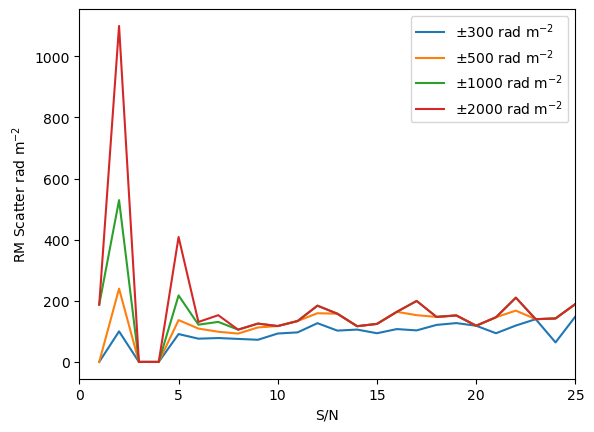
\includegraphics[width=\linewidth]{signal_to_noise.png}

        \caption[Rotation Measure scatter]{Plot showing scatter of RM as a function of signal to polarisation noise ratio for four Faraday depth search limits}
    \label{fig: s/n}
\end{figure}

With the signal-to-noise threshold found, I then created a rotation measure grid which showed the RM value found for each source with a signal to noise ratio above eight. The grid can be seen in Figure \ref{fig:1Grid} and shows a large variation across the field. The colour scale has been saturated at $\pm$ 400 rad$\,$m$^{\shortminus2}$ for ease of comparison with the Galactic latitude field in Figure \ref{fig: Shannon's RM grids}, however the RM values found range between a maximum of 696.8 rad$\,$m$^{\shortminus2}$ and a minimum of -697.3 rad$\,$m$^{\shortminus2}$. Within the Galactic plane the RM is mostly positive or zero however there are a few sources with a negative RM. This suggests that the magnetic field is being rotated clockwise as it passes through Faraday screen along the line of sight. These changes occur in over very short distances, so to get a better understanding of the scale of these changes I conducted a structure function analysis on the field. The density of RM sources can be seen to considerably decrease close to the bottom and left hand side of the field. This is due to the noisy edges contaminating these sources. This drop off in source density is not visible before the signal to noise ratio threshold is applied to the RM sources.



\begin{figure}
    \centering
    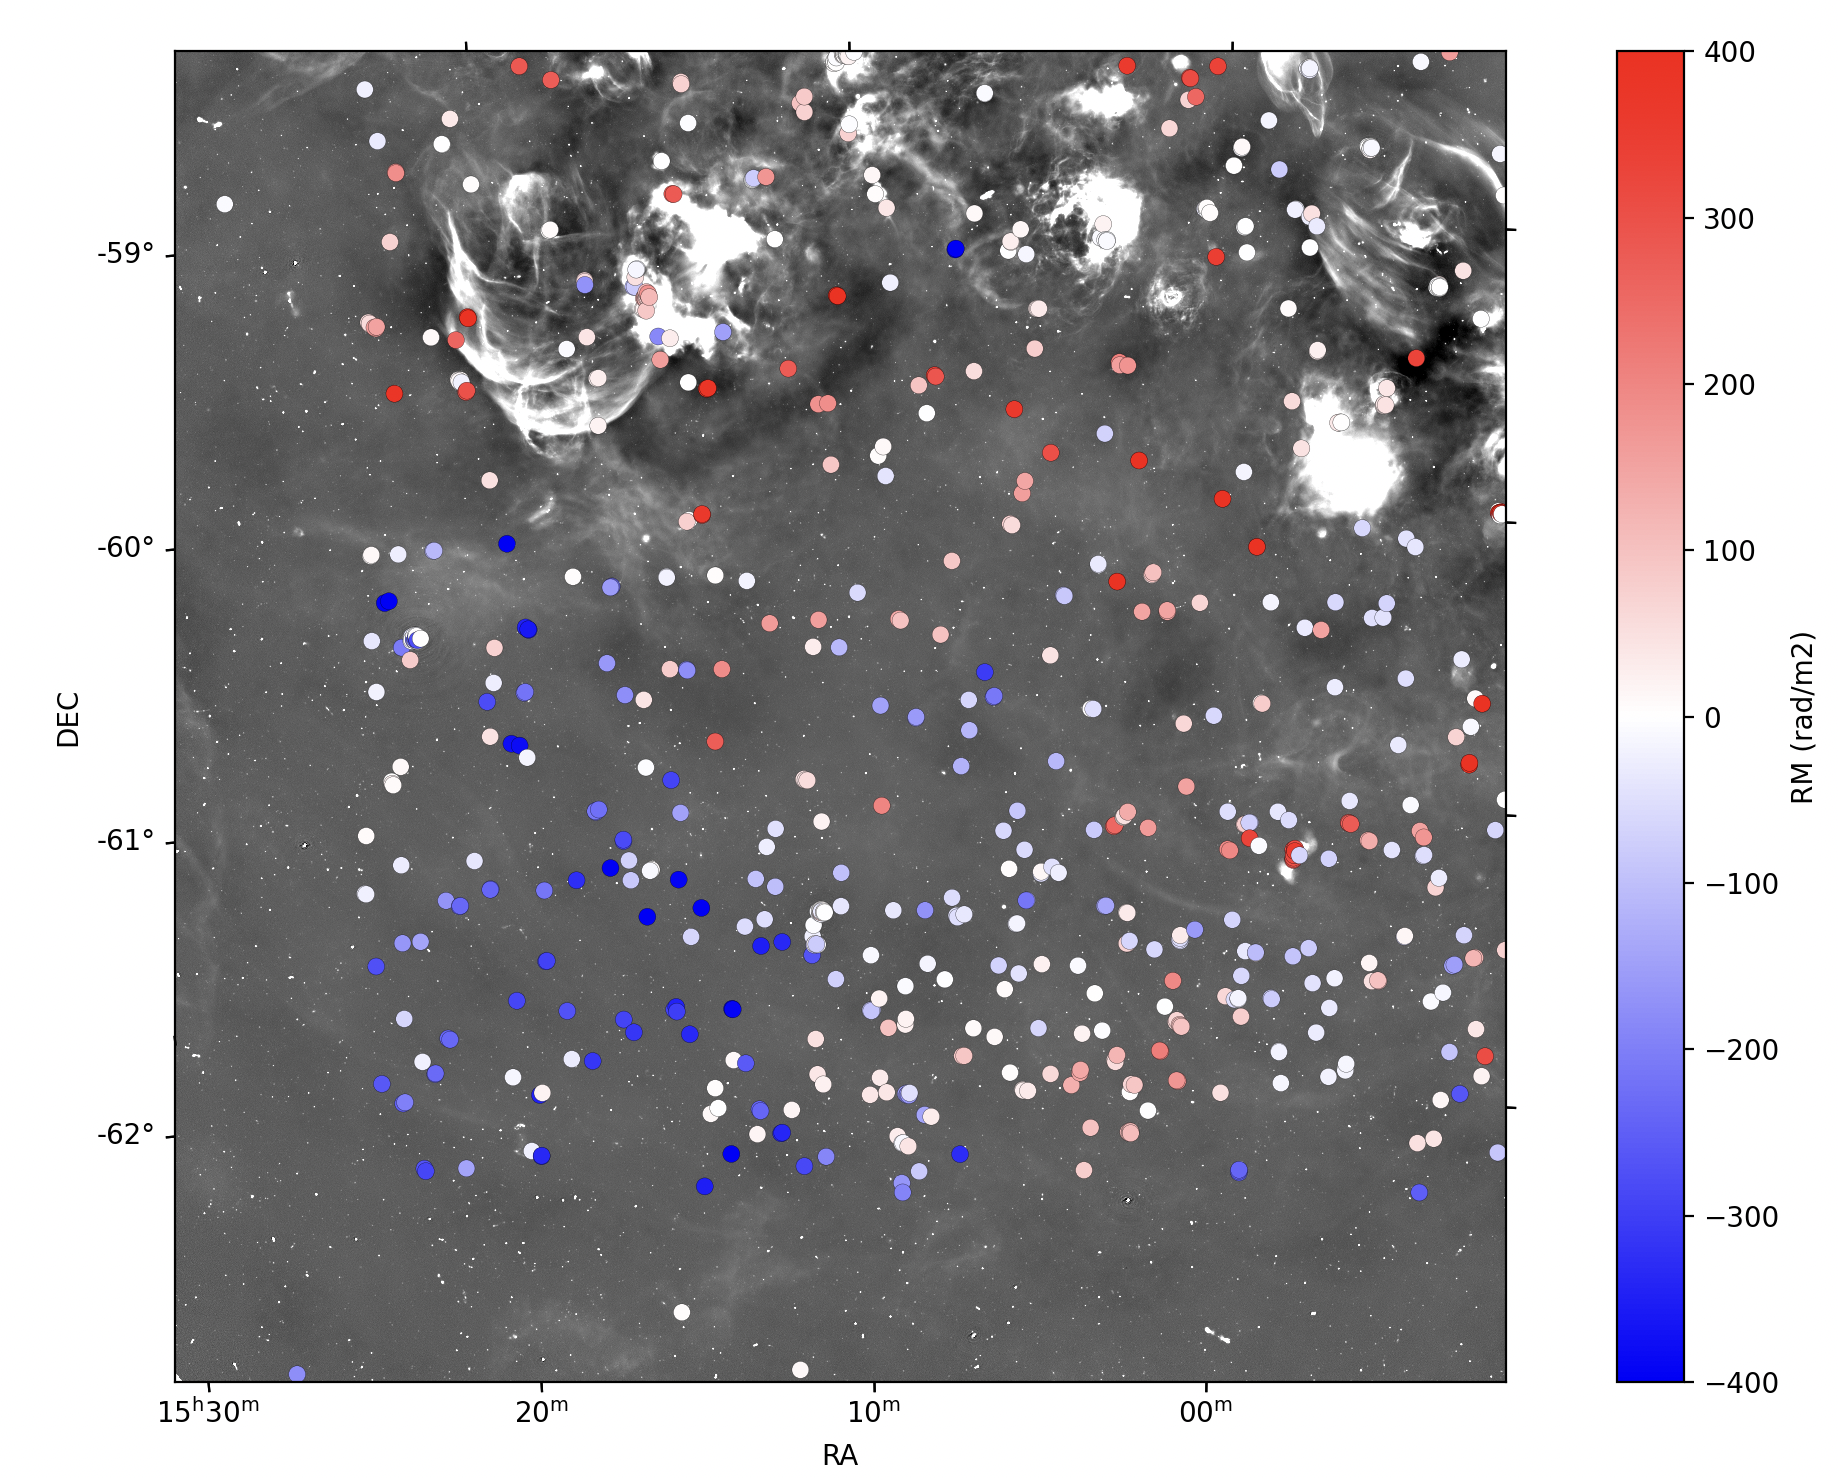
\includegraphics[width=\linewidth]{Thesis_Template/Figures/rm_without_nebulae.png}

        \caption[RM Grid]{RM grid showing the RM value for each source with a signal to noise ratio above 8, with red indicating a positive rotation measure and blue indicating a negative rotation measure. The colour scale is saturated at $\pm$ 400 rad$\,$m$^{\shortminus2}$}
    \label{fig:1Grid}
\end{figure}



\subsection{Structure Function Analysis}

Structure function analysis was performed in order to quantitatively understand the variation in RM across the field and the physical scale on which they occur.

The structure function equation gives a measure of the mean RM given a separation between two sources.

\begin{equation}
    STF(|\theta_i - \theta_j|) = \frac{1}{n}\underset{ij}{\Sigma}(RM(\theta_i) - RM(\theta_j))^2
    \label{Structure Function}
\end{equation}

\noindent where $\theta$ is the angular separation and $n$ is the number of sources in each bin (e.g. \cite{simonetti_1986}).

To apply this to the data I first removed any sources with a signal to noise ratio less than 8 from the catalogue, which left 823 sources. I next calculated the angular separation, $\theta$, and position angle between each pair of sources and created 18 bins between 0 and 360 arcseconds in angular separation and 6 bins between 0 and 180 arcseconds in position angle, where 0 is in the North-South direction. 

For each pair of sources I calculated the square of the differences and added it to the appropriate position bin. Finally I normalised the results by dividing by the number of pairs of sources in each bin, $n$. This is shown in Figure \ref{fig:2d_stf}. The lighter the structure function bin, the greater the variation of RM within the bin, so Figure \ref{fig:2d_stf} is showing that variation of RMs across the field varies most on scales of 300''-330'' angular separation and separations of 60''-90'' position angles.



\begin{figure}
        \centering
        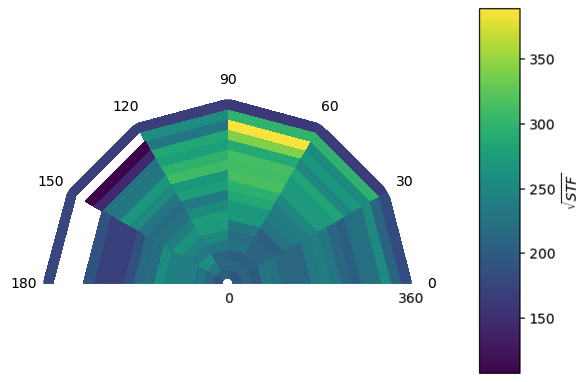
\includegraphics[width=\linewidth]{Thesis_Template/Figures/2D_STF.png}
        \caption[2D Structure Function]{2D structure function which shows the average rotation measure (in rad$\,$m$^{\shortminus2}$) given the separation between pairs of points in position angle and angular scale (both in arcseconds)}
        \label{fig:2d_stf}
    \end{figure}

In order to produce a one dimensional structure function, I then took the mean of all position angle bins for each separation angle bin, to produce Figure \ref{fig:1d_stf}.



\begin{figure}
        \centering
        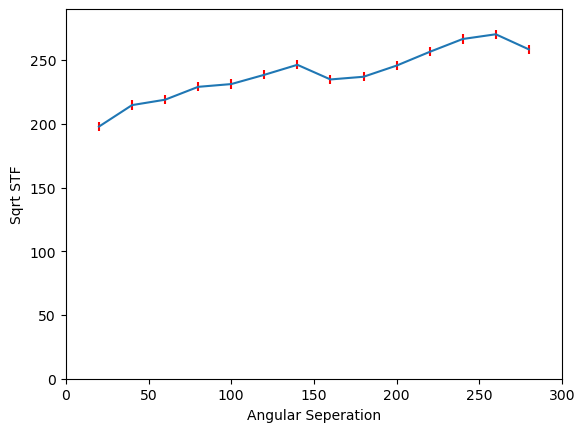
\includegraphics[width=\linewidth]{Thesis_Template/Figures/1D Structure Function.png}
        \caption[1D Structure Function]{1D structure function which shows the average rotation measure (in rad$\,$m$^{\shortminus2}$) as a function of angular separation (in arcseconds) between pairs of sources}
        \label{fig:1d_stf}
    \end{figure}

Both Figures \ref{fig:2d_stf} and \ref{fig:1d_stf}  show a general increasing trend of average rotation measure given two sources of increasing separation by both position angle and angular separation. The smaller difference, and blank sectors, seen towards the larger distance between sources in both position angle and angular separation in Figure \ref{fig:2d_stf} is due to very few, or no, pairs in those separation bins. Figure \ref{fig:2d_stf} shows a peak in the structure function in the position angle bin between $60^\circ$ and $90^\circ$, which is along the Galactic plane. This suggests that RM varies more along the plane than perpendicular to it. It is also interesting to note the steep rise to a high value for the structure function at such low separations, most clearly visible in Figure \ref{fig:1d_stf} but can also be seen in Figure \ref{fig:2d_stf}. This consistently high difference between RM at all separations suggests that there is rapidly varying small scale structure within the magnetic field of spiral arms. 

The field EMU1505-60 has a galactic longitude of approximately 319$^\circ$. Using the diagram of the Milky Way shown in Figure \ref{fig:mw map} to estimate distances, the line of sight first passes through the Sagittarius arm at a distance of approximately 1$\,$kpc, then the Scutum-Centaurus spiral arm twice at approximately 4$\,$kpc and 13$\,$kpc and finally the Sagittarius arm again at 17$\,$kpc. The emission and rotation from hte arms likely play a role in the variation seen in this RM grid.

\begin{figure}
    \centering
    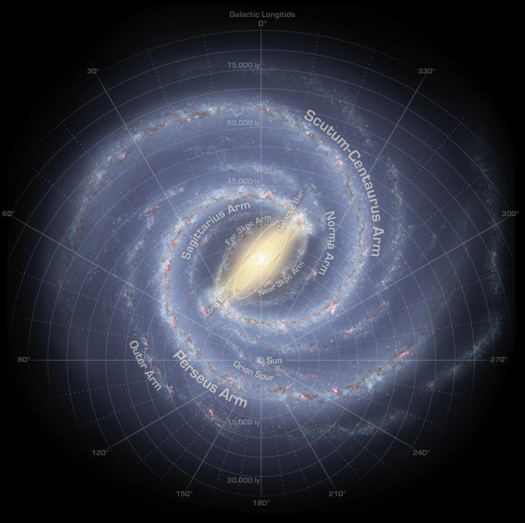
\includegraphics[width=\linewidth]{Thesis_Template/Figures/Milky Way Map.png}
    \caption[Diagram of the Milky Way]{Diagram of Milky Way with spiral arms and Galactic longitude labels, taken from \cite{spitzer_2009}}
    \label{fig:mw map}
\end{figure}

These angular scales correspond to variations of RM on scales of approximately 1$\,$pc at the first crossing of the Sagittarius arm, and 3$\shortminus$9$\,$pc at the two crossings of the Scutum-Centaurus spiral arm and 12$\,$pc variations at the second Sagittarius crossing. This result shows variation on a smaller scale than previous results which show variation on scales of $\sim$12$\shortminus$24$\,$pc at a distance of 1$\shortminus$2$\,$kpc (\cite{vanderwoude2024prototypefaradayrotationmeasure}, \cite{Haverkorn_2006}). This could suggest that this line of sight is more dominated by diffuse emission from the secondary passing of the Scutum-Centaurus band. Investigations of this over larger fields that will be possible when more fields from POSSUM are available will allow for a better understanding. 

%log plot to compare to vanderwoude and haverkorn?


 
\chapter{Diffuse Polarisation}
\label{ch: Canals}

The previous two chapters have described the work I have done to increase the number of RM values found for extragalactic sources within the diffuse emission of the Galactic plane. This chapter showcases the results of the 3D rotation measure synthesis pipeline, and further analysis, which progresses our understanding of the diffuse polarisation within the Galaxy.

\section{Evolution of Diffuse Polarisation Measurements }

Characterising the polarisation of Galactic diffuse emission is a relatively new field, begun by work by \cite{Wieringa_1993}. This work found various structures present in observations of diffuse polarised emission. These observations were taken using the Westerbork Synthesis Radio Telescope (WSRT) at 325 MHz at high Galactic latitudes. These structures were seen on a variety of scales down to a few arcminutes and do not have an apparent counterpart in observations of total intensity. This work also compared these observations to numerical simulations of interferometric observations of a uniformly polarised background which suggested that qualitatively, this is a good description of the observations.

Further observations were taken by WSRT in the frequency range 341-375 MHz (e.g. \cite{Haverkornetal_2000}, \cite{Haverkorn_2001}, \cite{Haverkorn_2004}) which analyse in greater detail the structures present. 
%One key structure described are depolarisation canals. These canals are narrow, filament-like one dimensional structures and have a very low polarised intensity.
There has also been pioneering work done at lower frequencies by \cite{Bernardi_2009}. This work also used WSRT to characterise the foreground emission for epoch of reionisation experiments, probing an area of the sky at a low Galactic latitude within 140-160${\rm\,MHz}$. 

POSSUM has allowed us to probe more of the Galaxy as it uses higher frequencies, i.e. 943$\,{\rm MHz}$, and has pointings closer to the Galactic centre, meaning that the radiation observed has a longer path through the diffuse emission of the Galactic plane. Diffuse polarisation had not been seen before at such high frequencies as before ASKAP and MeerKAT, such high frequencies were not covered by synthesis arrays. Higher frequencies, and thus shorter wavelengths, result in a larger maximum scale of detectable structures in Faraday space as

\begin{equation}
    \phi_{max-scale} = \frac{\pi}{\lambda_{min}^2}
\end{equation}

(e.g. \cite{Sun_2015}). This in turn means that emission with wider peaks in FD can be detected and as more distant material will have a larger range of RM in a fixed beam size for a given RM gradient, and thus a wider FDF, this emission can be seen.

Another advantage of POSSUM is the smaller beam size, which means that the RM distribution can be better resolved. However, for the polarised emission to be visible, the RM gradients also have to be large enough to divide Stokes Q and U into small enough regions to detect on short baselines. This, combined with the limit in terms of FDF as described above are why the features that are visible in polarised intensity do not have corresponding features in total intensity.




%Another possible explanation for the depolarisation canals is a rapid switching between multiple peaks of RM. %I can remember reading something about this but I can't find it now - grr

%This quick change in RM value could result in a steep gradient, and if positioned in a certain way could produce canal like structures. %I'm like 90% sure what I've have just written is wrong!



\section{3D Pipeline}
\label{3d pipeline}

In order to investigate the diffuse polarisation of the field 1505-60 I first ran the 3D POSSUM polarimetry analysis pipeline

This implementation of this pipeline consists of three steps: creating the spectral model, 3D RM synthesis and peak fitting.

The first step fits a model to the Stokes I data cube using RM-tools' fitIcube routine. This script fits Stokes I models pixel-wise using the 1D fitting routine to the Stokes I data cube. This model cube is created using the same power law as used for the model Stokes I spectrum found for each source as part of the one dimensional pipeline.

The second step of the pipeline has two main parts. First it uses the model cube calculated to find the fractional polarisation and then it performing 3D RM synthesis which uses the rmsynth3D routine from RMTools to perform a non-gridded discrete Fourier transform, from Equation \ref{eq: discrete rm synth}, to calculate the FDF. The weighting of this data was chosen to be inverse variance again to reduce the noise in the FDFs. 
The spacing between samples and maximum distance over which Faraday depth is defined is also calculated in the same way as for the 1D synthesis. 
The third and final step of this pipeline is peak fitting. This step uses the RMpeakfit$\_$3D routine from RM-tools to apply the one 
dimensional RM spectrum characterisation and peak fitting techniques using the same method as the peak fitting described in the extract spectra step of the one dimensional pipeline and then applies it pixelwise to the three dimensional FD cube. This step produces 2D maps of rotation measure and polarised intensity.

Descriptions of the outputs of this pipeline can be found in Appendix \ref{AppA: 3D pipeline output}.

The results of the 3D polarimetry analysis pipeline on the field EMU1505-60 yielded a 2D map of the peak polarised intensity, Figure \ref{fig: pi map}, and rotation measure, Figure \ref{fig: rm map}. 

\begin{figure}
    \centering
    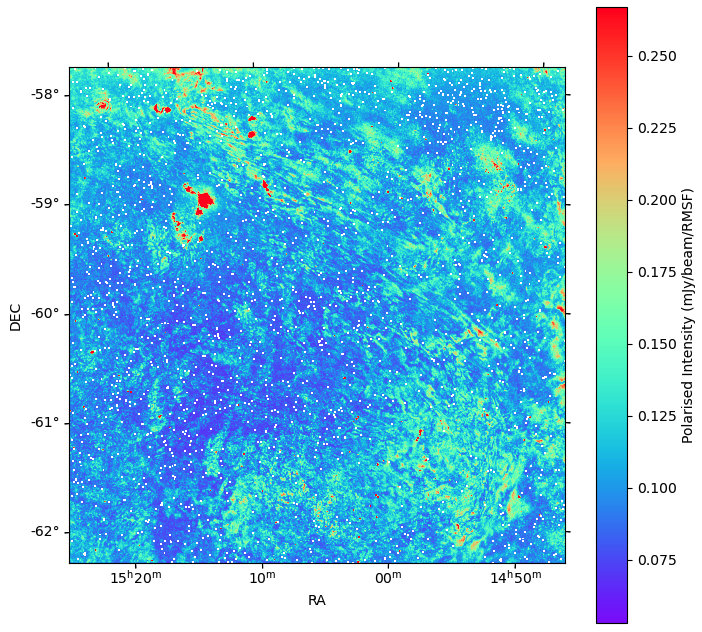
\includegraphics[width=1\linewidth]{Thesis_Template//Figures/Pi map.png}
    \caption{Polarised Intensity Map of EMU1505-60}
    \label{fig: pi map}
\end{figure}

\begin{figure}
    \centering
    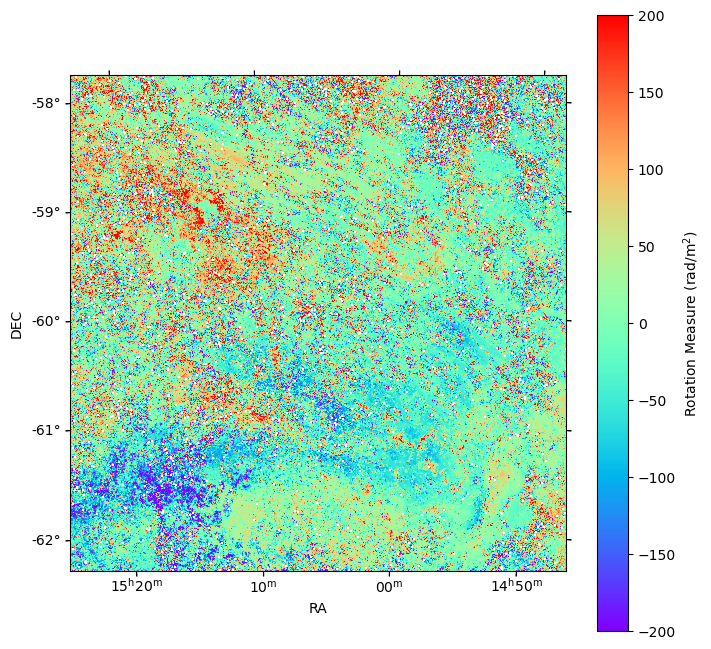
\includegraphics[width=1\linewidth]{Thesis_Template//Figures/RM map.png}
        \caption{Rotation Measure Map of EMU1505-60}
    \label{fig: rm map}
\end{figure}

Figure \ref{fig: pi map} demonstrates that there is polarised emission present across the entire field, which is interesting as it does not match the structure and distribution of the total intensity. The whole field is full of smooth, high-brightness diffuse synchrotron emission, visible in single-dish maps. This is resolved out in this synthesis image, leaving only structures with scales less than half a degree. The Faraday effect breaks up the polarised intensity, making it more unstructured, which can be seen as the 'blobby' pattern, most prominent across the right hand side of the image (see Figures \ref{fig: blobby zoom} and \ref{fig: canals zoom}). The supernova remnant MSH15-22 can be seen clearly in the upper left corner of the image as an extended peak in polarised intensity and can be seen in more detail in Figure \ref{fig: sn zoom}.

\begin{figure}
    \centering
     \begin{subfigure}[b]{\textwidth}
        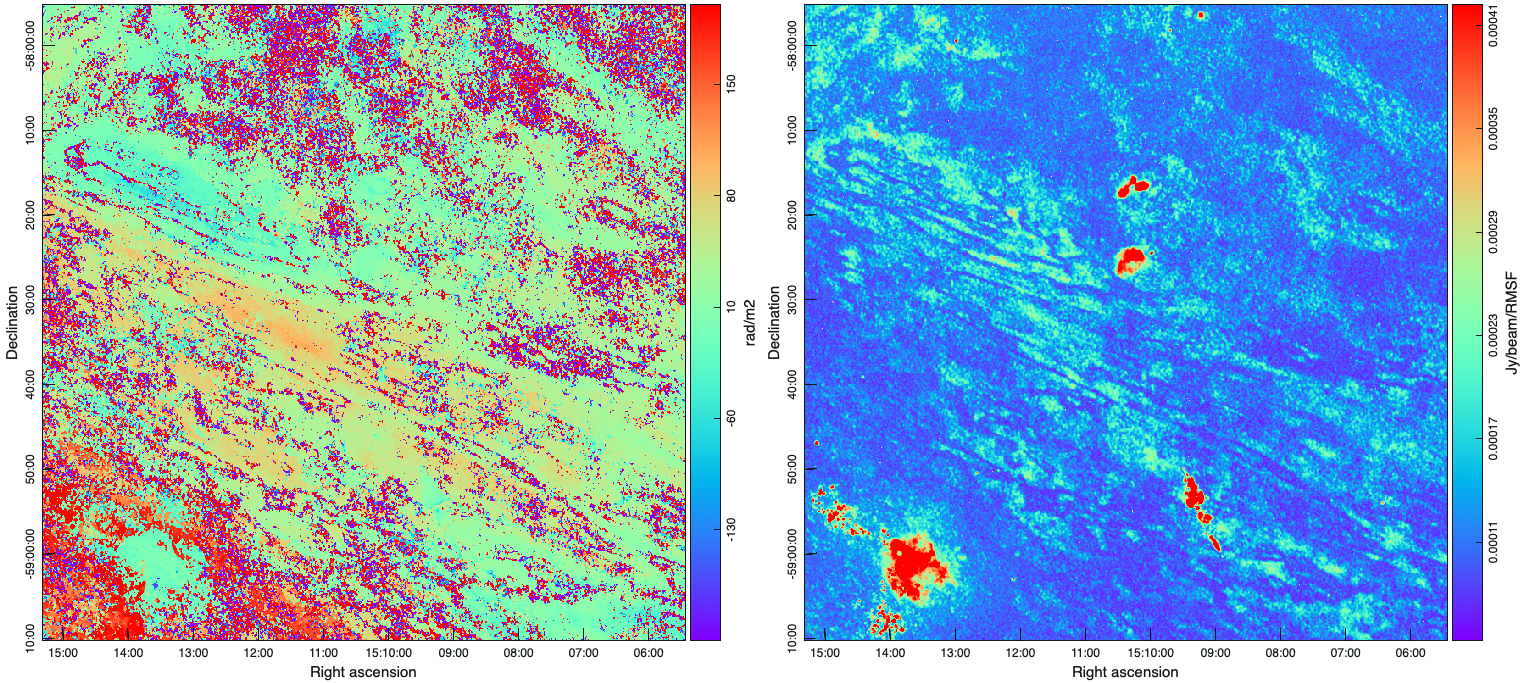
\includegraphics[width=\linewidth]{Thesis_Template/Figures/RM_PI top right.png}
        \caption{Structure dominated by long filament like canals which can be seen in both RM and PI maps}
        \label{fig: canals zoom}
    \end{subfigure}

    
    \vspace*{0.05cm}

    
    \begin{subfigure}[b]{\textwidth}
        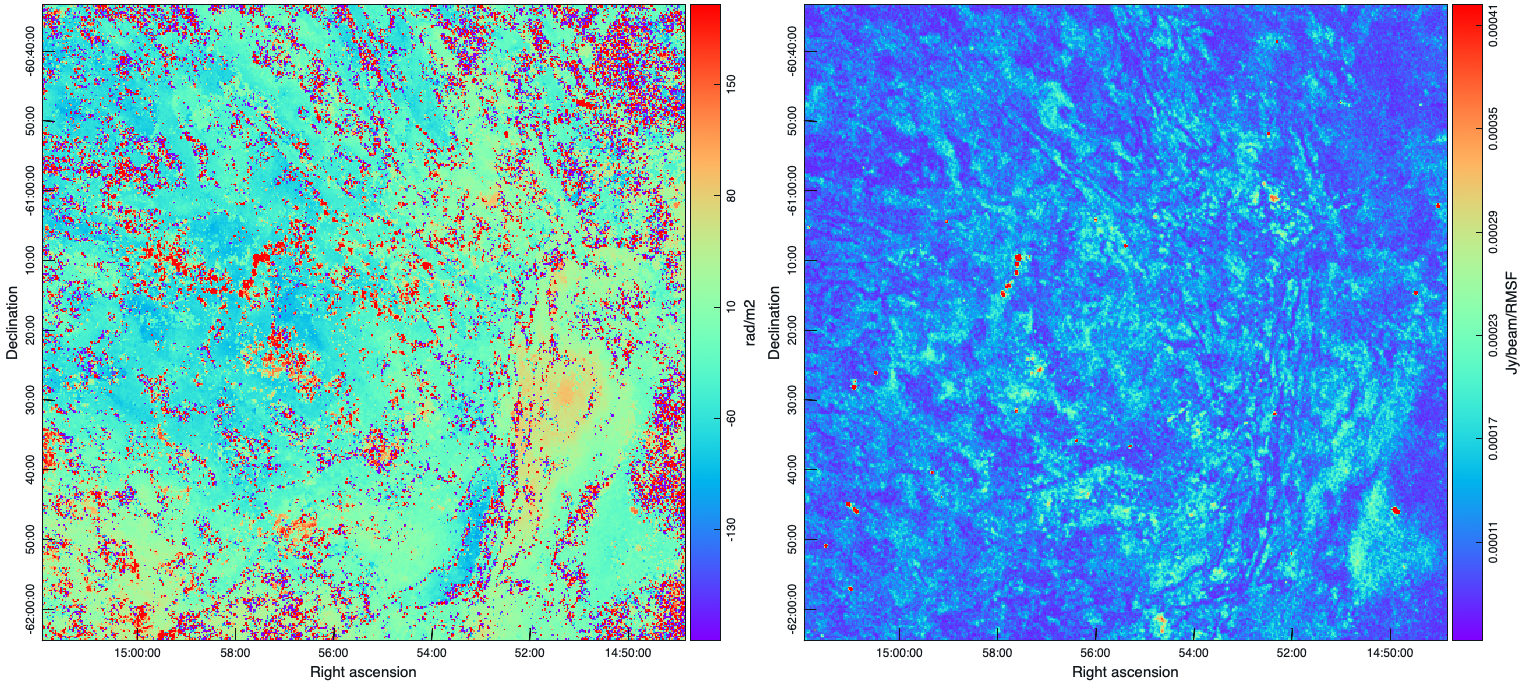
\includegraphics[width=\linewidth]{Thesis_Template/Figures/RM_PI bottom right.png}
        \caption{Blobby structure can be clearly seen in the PI map, with varying corresponding RM. Canal-like structure can also be seen in this region}
        \label{fig: blobby zoom}
    \end{subfigure}

    
    \vspace*{0.05cm}

      \begin{subfigure}[b]{\textwidth}
        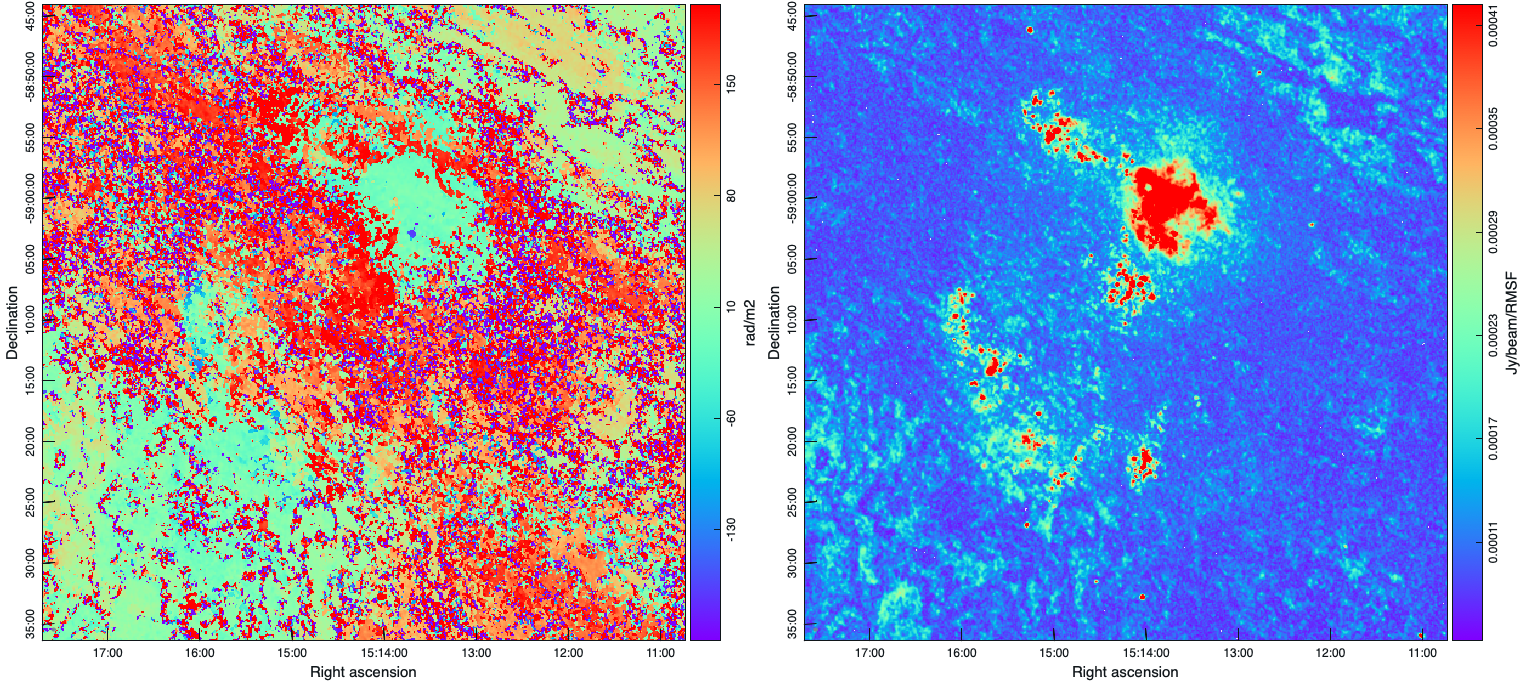
\includegraphics[width=\linewidth]{Thesis_Template/Figures/RM_PI_MSH 15-22.png}
        \caption{Supernova remnant MSH 15-22, which can be seen as a peak in the PI map, but has a low magnitude in the rotation measure map}
        \label{fig: sn zoom}
    \end{subfigure}
    

   
    
    \caption{Zoomed in figures of interesting features in Rotation measure (left) and Polarised Intensity (right) maps for field EMU1505-60}
    \label{fig:pi and rm zooms}
\end{figure}



This map has not been corrected for Ricean bias, which is a positive bias which arises from the contribution of the difference between the measured and true values for Stokes Q and U. However, as I have blanked all values with a signal to noise below 2, the contribution of this bias is minimal.

Another interesting feature which can be seen in both these Figure \ref{fig: pi map} and Figure \ref{fig: rm map} is canal like structures, particularly in the upper right hand quadrant of the polarised intensity map (see Figure \ref{fig: canals zoom}). Canal-like structures have also been identified in many other POSSUM fields by Dr Jennifer West (priv. comm.).

These canals are parallel to the Galactic plane, which means that they are parallel to the projected magnetic field of the Galaxy, as measured by \cite{Planck_XXV}. They also run parallel between the RM and PI maps, which implies that the RM gradient is perpendicular to the canals. Further quantitative analysis of the RM gradient is described in Section \ref{grad analysis}. There have been two predominant explanations for these canals put forward. One proposed by \cite{Haverkornetal_2000} suggests that beam depolarisation is responsible. Beam depolarisation is caused when the polarisation angle varies significantly within a beam such that for each line of sight there is a complementary line of sight that has the same polarised intensity, but the polarisation angle is shifted by 90$^\circ$. This was believed to be the case because it was found that the polarisation angle changes by 90$^\circ$ across the beam. This does not account for why the patterns of canals vary with wavelength.

The other is that they are instead caused by differential Faraday rotation in the interstellar medium. %\cite{beck}. 
\cite{Shukurov_and_Berkhuijsen_2003} built on this theory by proposing that the canals are in fact due to multiples of RM where $RM = RM_0 \equiv n\pi / (2\lambda^2)$ with $n$ being integer multiples. Their model follows Burn's sinc law (\cite{burn_1966}) which is zero when the intrinsic Faraday rotation is rotated by exactly $\frac{\pi}{2}$, $\frac{3\pi}{2}$ etc. This model would mean that the depolarisation varies more smoothly as the width of the canal is set by the RM gradient, rather than the beam size.

\section{Structure Detection}

Before conducting further analysis on the structure within these maps it is important to verify that the structure is that the interferometric observation has not fully detected this structure and that it is in fact just an artefact of the observational technique, such as the large fractional variations in Stokes Q and U observed could instead actually be small perturbations on a very smoothed polarised structure that has been resolved out. If this were the case, the polarisation angles would be much more uniform over the field (\cite{Haverkorn_2004}). In order to investigate this further, I conducted the 3D RM synthesis on the same field, EMU1505-60, but with only the lowest 100 frequency channels, which have a $\lambda^2$ range of between 0.11-0.14$\,$rad$\,$m$^{\shortminus2}$. The full frequency range gives a corresponding $\lambda^2$ range of 0.076-0.14$\,$rad$\,$m$^{\shortminus2}$. If this structure has not been fully detected, it should be better detected at lower frequencies because larger changes in angle for a given RM gradient would be more likely to remove the large-scale component which we can't detect, but would change the RM map. Therefore, by comparing the full band and the lower section of the band, we will be able to see the completeness of this structure. 

I compared the rotation measure and polarised intensity across the entire frequency range to the lower frequency range by creating Figures \ref{fig: rm vs lower} and \ref{fig: pi vs lower}. These plots only show values for which the error of the lower frequency range is less than 3 rad$\,$m$^{\shortminus2}$, which leaves 39$\%$ of the total number of pixels.

\begin{figure}
    \centering
    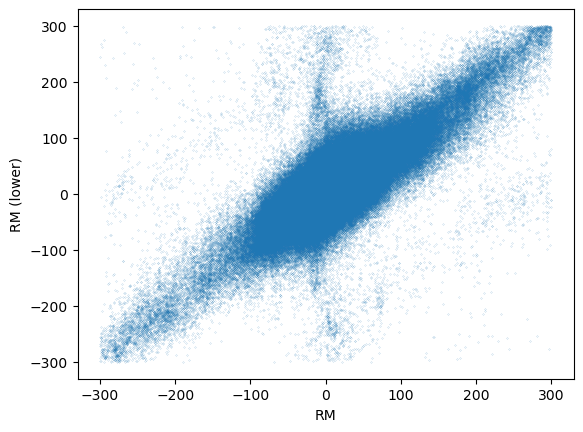
\includegraphics[width=1\linewidth]{Thesis_Template/Figures/RM_vs_lower.png}
    \caption{Plot of rotation measure across the full frequency channel range in rad$\,$m$^{\shortminus2}$ against the polarised intensity across the lowest hundred frequency channels.}
    \label{fig: rm vs lower}
\end{figure}

\begin{figure}
    \centering
    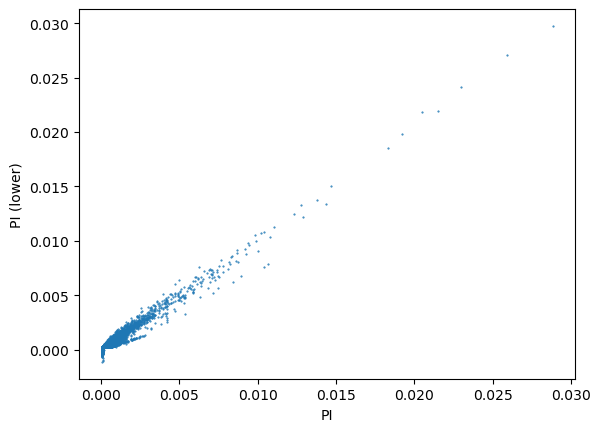
\includegraphics[width=1\linewidth]{Thesis_Template/Figures/PI_vs_lower.png}
    \caption{Polarised intensity across the full frequency channel range in Jy/beam/RMSF 
    against the rotation measure across the lowest hundred frequency channels.}
    \label{fig: pi vs lower}
\end{figure}

Both plots show a strong positive correlation with a gradient close to 1 between the full and the lower frequency ranges, which indicates that the same structure is detected in both the lower frequency section and across the complete frequency band. Therefore, this diffuse structure is real. Some outliers within RM can be seen around one in the full band, but with values across the whole range in the lower band. An explanation for this is still required as there is not an obvious cause for this, however these outliers make up only $0.2\%$ of the RM values.


\section{Peak Fitting}

There are two different broad categorisations of Faraday spectra: Faraday simple and Faraday complex (\cite{Alger_Livingston_McClure-Griffiths_Nabaglo_Wong_Ong_2021}, \cite{thomson2023rapidaskapcontinuumsurvey}, \cite{vanderwoude2024prototypefaradayrotationmeasure}). Faraday simple refers to spectra that have a single peak in the form of a delta function, which gives an unambiguous RM value. If there is more than one peak in the spectra, or the peak has a finite width, it is referred to as Faraday complex. One possible cause for Faraday complexity is multiple synchrotron emitting regions with different RMs along the same line of sight, for example, background and foreground emission from a supernova remnant. This would appear in the Faraday spectrum as multiple peaks or a Gaussian broadening such that the peak cannot be resolved. A scenario such as this would lead to depolarisation. 

In order to investigate the occurrence of multiple peaks within the rotation measure, I utilised code written by Dr Vasu Shaw
to identify spectra with multiple peaks and make maps of the RM values of the individual peaks. 
%Where multiple peaks are found, they are ordered by magnitude, with the primary being the largest. 
The primary peak, Figure \ref{fig: peak 1}, was consistent with the result from the pipeline.

\begin{figure}
    \centering
    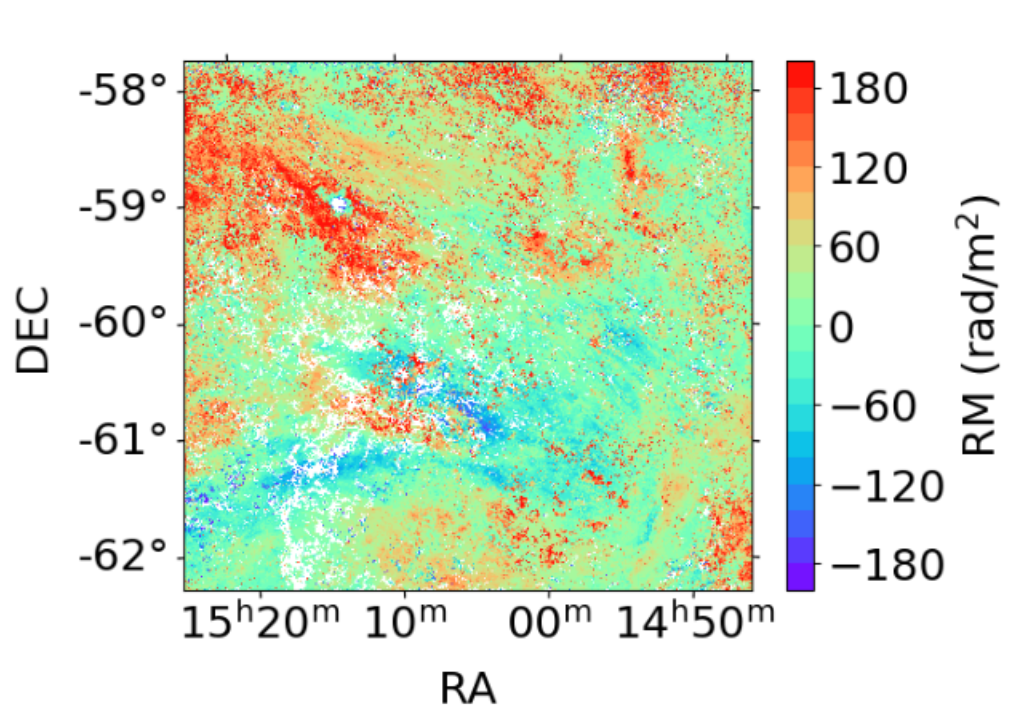
\includegraphics[width=\linewidth]{Thesis_Template/Figures/Peak 1.png}
    \caption{The primary peak in the FDF cube for field EMU1505-60.}
    \label{fig: peak 1}
\end{figure}


\begin{figure}
    \centering
    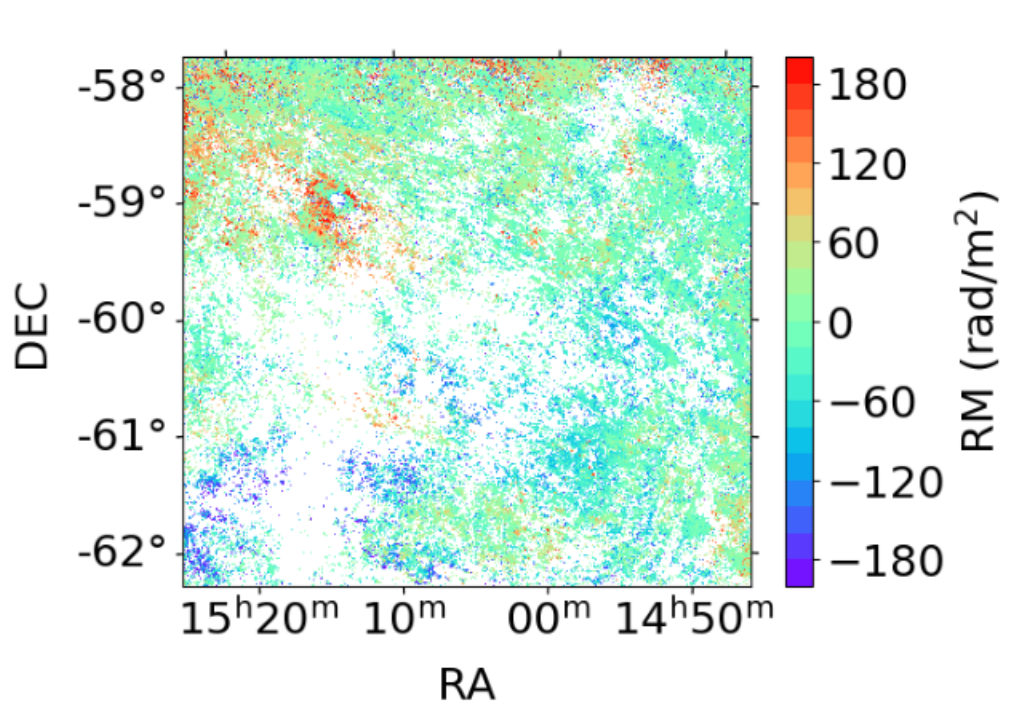
\includegraphics[width=\linewidth]{Thesis_Template/Figures/Peak 2.png}
    \caption{The secondary peak in the FDF cube for field EMU1505-60.}
    \label{fig: peak 2}
\end{figure}

\begin{figure}
    \centering
    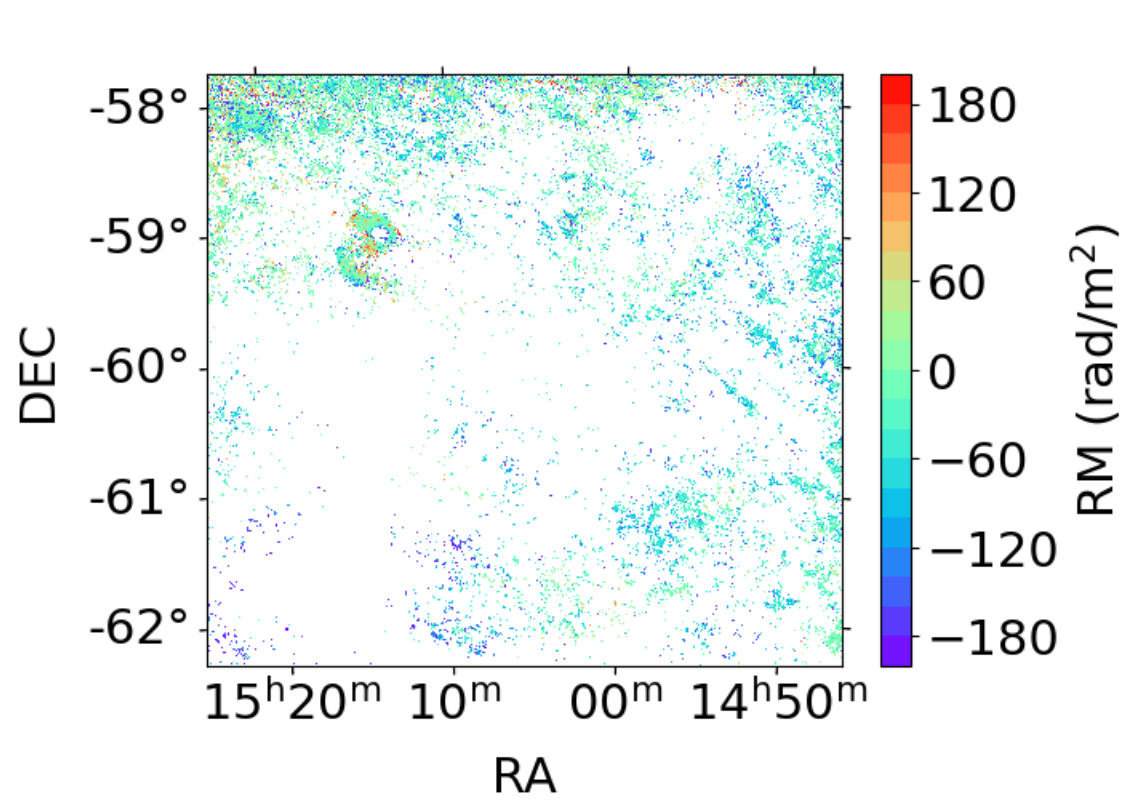
\includegraphics[width=\linewidth]{Thesis_Template/Figures/Peak 3.png}
    \caption{The tertiary peak in the FDF cube for field EMU1505-60.}
    \label{fig: peak 3}
\end{figure}

Figures \ref{fig: peak 2} and \ref{fig: peak 3} demonstrates that there are multiple peaks within the FDF cube. The secondary and tertiary peaks by visual inspection appear to have a similar value to the primary peak, which suggests that there is not a large difference between the peaks which could lead to a depolarisation canal to be seen. These results therefore do not support the explanation that multiple peaks are responsible for the canal phenomena.

For POSSUM, the maximum detectable scale for RM synthesis is smaller than the width of the RMSF, so such features as multiple peaks can't be clearly and correctly resolved. If the spread is less than the maximum scale, but not negligibly small, then FDF peak will be slightly wider than the RMSF. A broad FDF component will disappear if it is a smooth peak or produce peaks which are not real but in fact detections of the distribution edges (\cite{Erceg_2022}). This would explain why the multiple peaks observed are close to each other in FD.

\section{Gradient Analysis}
\label{grad analysis}

Conducting gradient analysis of the rotation measure cube allows for a more quantitative investigation of the canal features. One of the products of the complete POSSUM pipeline will be 3D RM synthesis images of the whole survey, and as part of this process RMclean (\cite{Heald_2009}) will be applied, which will reduce interference from the sidelobes of the RMSF. This step had not been done on the field previously analysed in this dissertation. Dr Roland Kothes has used a separate analysis of the publicly available Stokes I, Q and U cubes from POSSUM at low Galactic latitudes via the same process as the POSSUM pipeline, but without mosaicking the separate fields toegther as will be done for POSSUM. Also no correction for the ionospheric Faraday rotation has been made, however as this does not cause structure or depolarisation this lack of correction would not affect the outcome of this analysis. Therefore I have used on of these processed fields, EMU1615-64, to conduct gradient analysis. This field was chosen as it showed the most prominent example of the canal-like filaments of interest, however these structures could be seen in many POSSUM fields.

For this analysis I used NINER to apply gradient masks. I applied a gradient mask for North, East, South and West to the rotation measure map (which is shown in Figure \ref{fig:1615-64 rm}). These masks can be found in the NINER documentation\footnote{NINER documentation can be found at http://www.aips.nrao.edu/cgi-bin/ZXHLP2.PL?NINER} \footnote{A bug was found within NINER which has resulted in the masks producing gradients in the opposite direction to those expected. This was adjusted for manually.}. I then rotated averaged the opposite directions, i.e. North and South, East and West and then found the average between these pairings. Finally, I calculated the direction and magnitude of the gradient at each pixel. By normalising and using an HSV image, converting the direction into the hue value and the magnitude into a brightness value I created Figure \ref{fig:hue} to highlight the depolarisation canals. The bright areas in this figure show areas of large gradient, with the stripes of colour representing lines with a consistent angle of gradient. These can be seen at a variety of orientations with large magnitudes, especially within the centre of the image. The bright areas without extended gradient features are due to regions of low signal to noise where the jumps in RM are due to noise rather than true features. The black regions are regions with no value for RM and very low PI. By comparing this map to the PI map (Figure \ref{fig:1615-64 pi}) it can be seen that not all gradients found have a corresponding feature in PI. An example of a canal feature in PI corresponding to a change in RM and thus a clear gradient in the gradient map is shown in Figure \ref{fig: 1615 zoom}. The prominent feature in C, the green filament can be seen to correspond to the change between an RM of $\sim 175$ and $\sim 125\,$rad$\,$m$^{\shortminus2}$. This also partially corresponds to a canal in PI, however this does not follow the full line of change in RM.

\begin{figure}
    \centering
    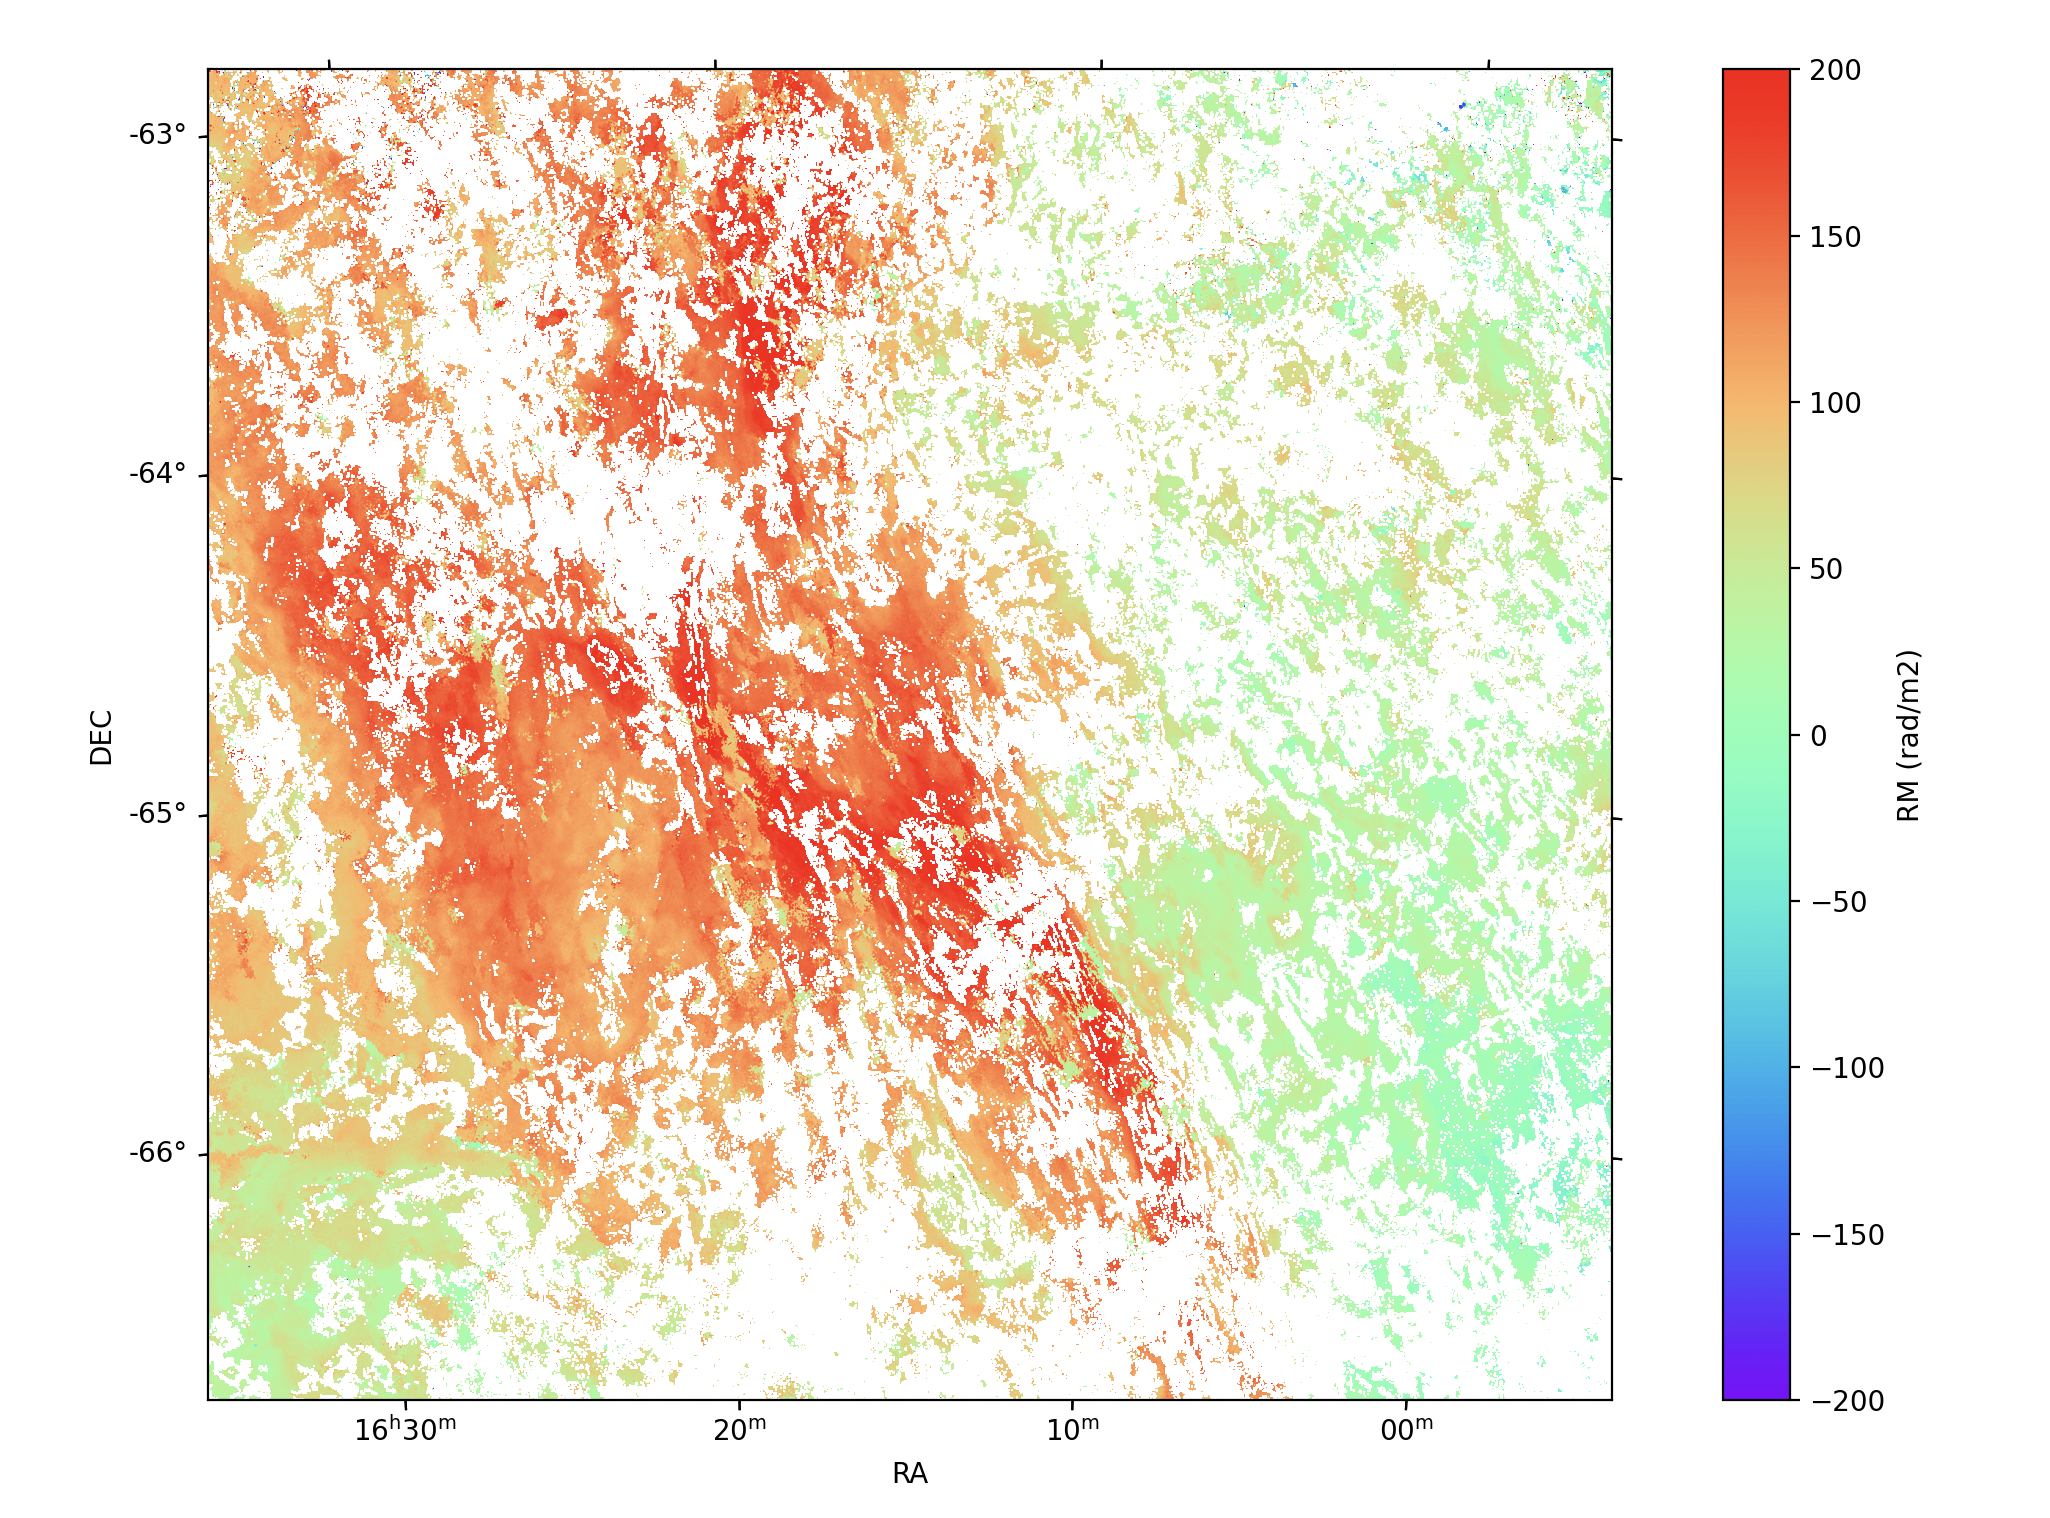
\includegraphics[width=1\linewidth]{Thesis_Template/Figures/1615-64_RM.png}
    \caption{Rotation Measure map of EMU field 1615-64.}
    \label{fig:1615-64 rm}
\end{figure}

\begin{figure}
    \centering
    \includegraphics[width=1\linewidth]{Thesis_Template/Figures/1615-64_PI.png}
    \caption{Polarised Intensity map of EMU field 1615-64.}
    \label{fig:1615-64 pi}
\end{figure}

\begin{figure}
    \centering
    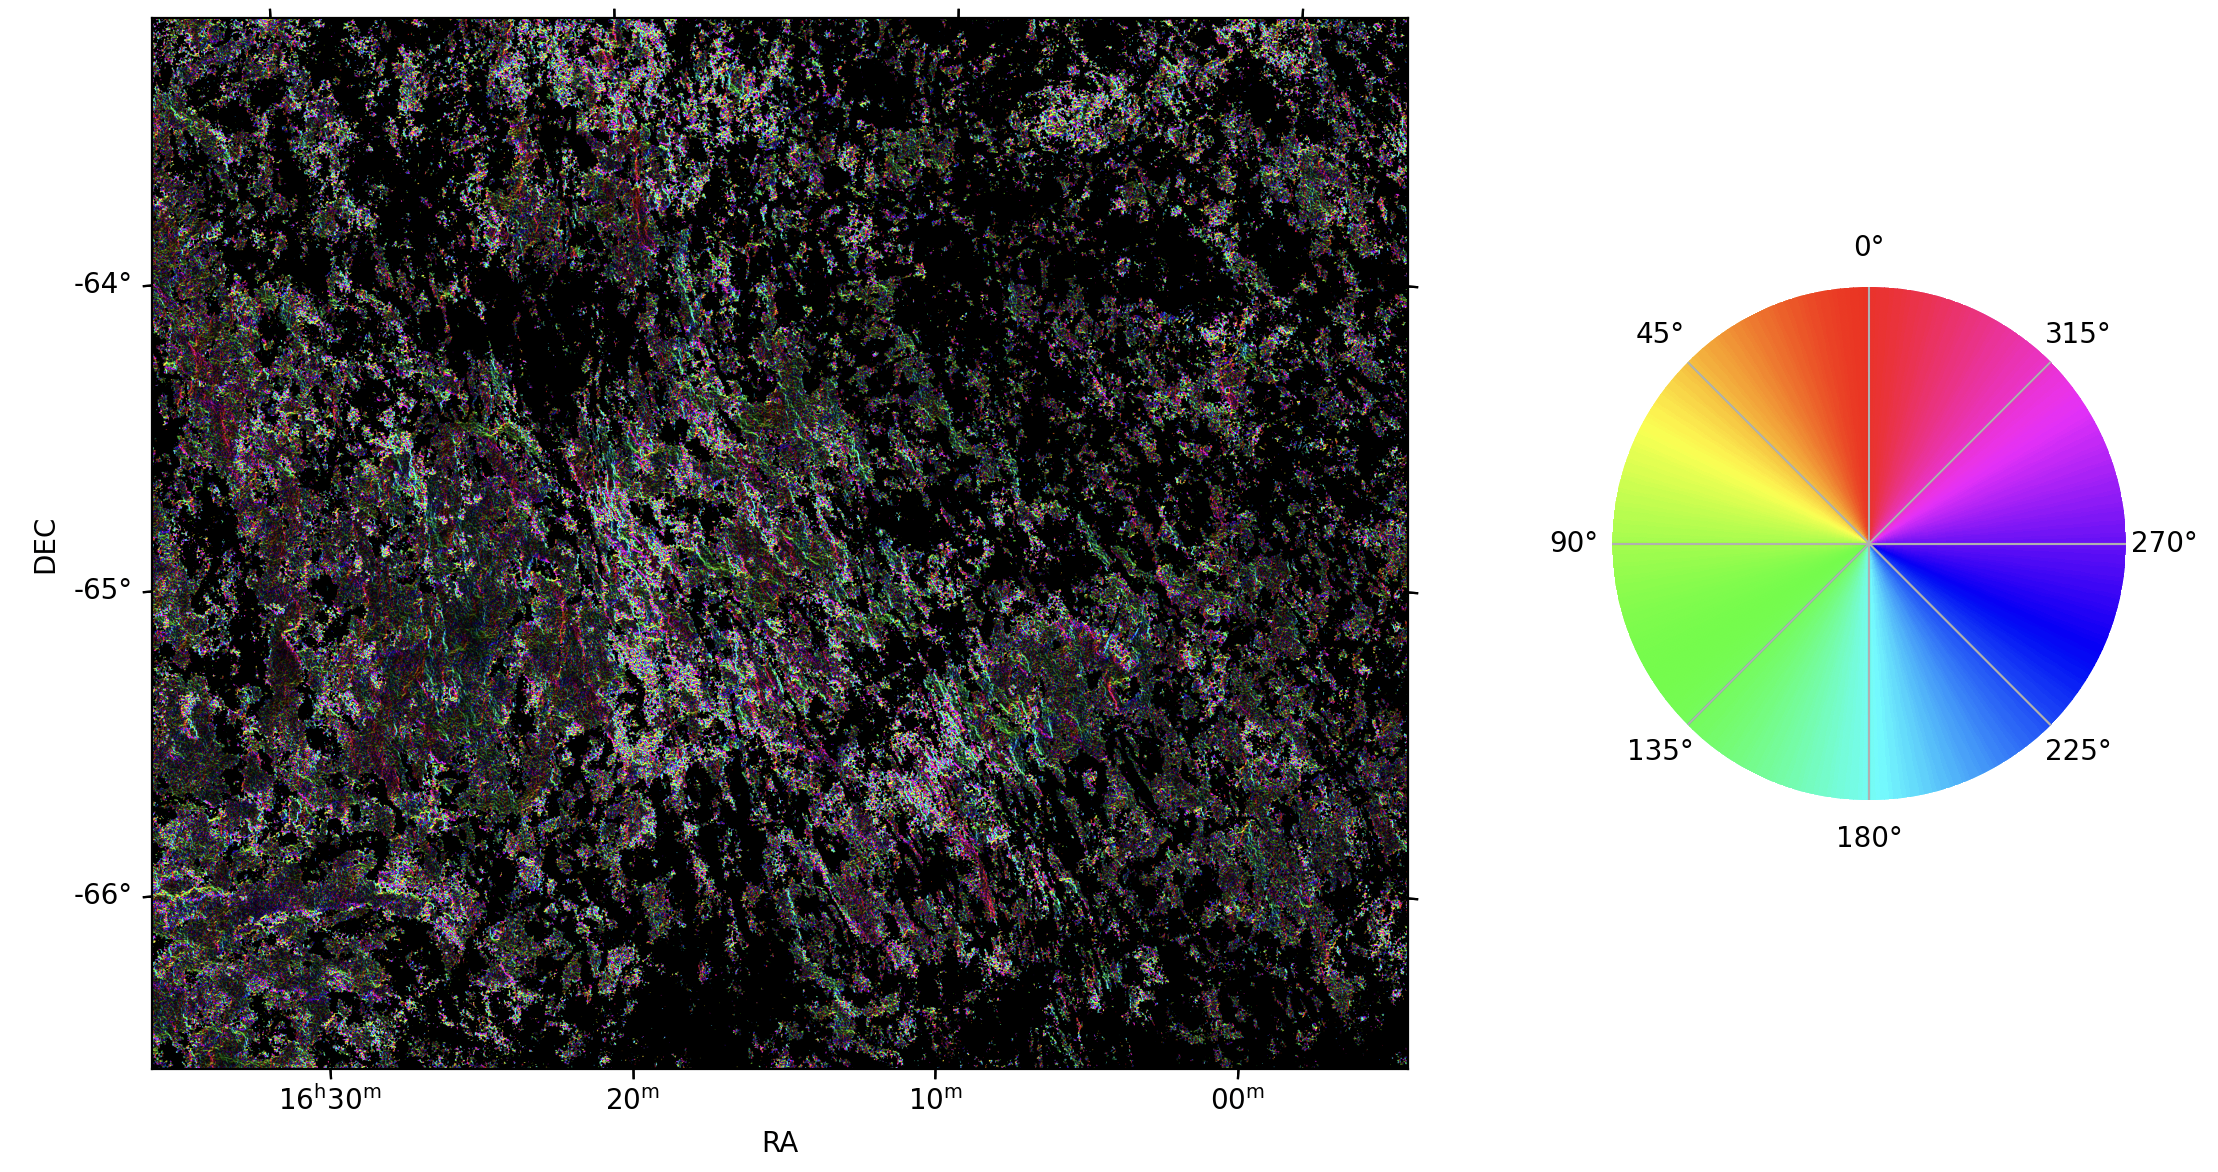
\includegraphics[width=\linewidth]{Thesis_Template/Figures/Hue_3.png}
    \caption{Map of angle and amplitude of the gradient of field EMU1615-64. The colour of the pixel represents the angle of the gradient at that point, and the brightness of the colour represents the amplitude of the gradient at that point, with a higher brightness representing a larger amplitude of gradient. }
    \label{fig:hue}
\end{figure}

\begin{figure}
    \centering
    \begin{subfigure}[b]{0.6\textwidth}
        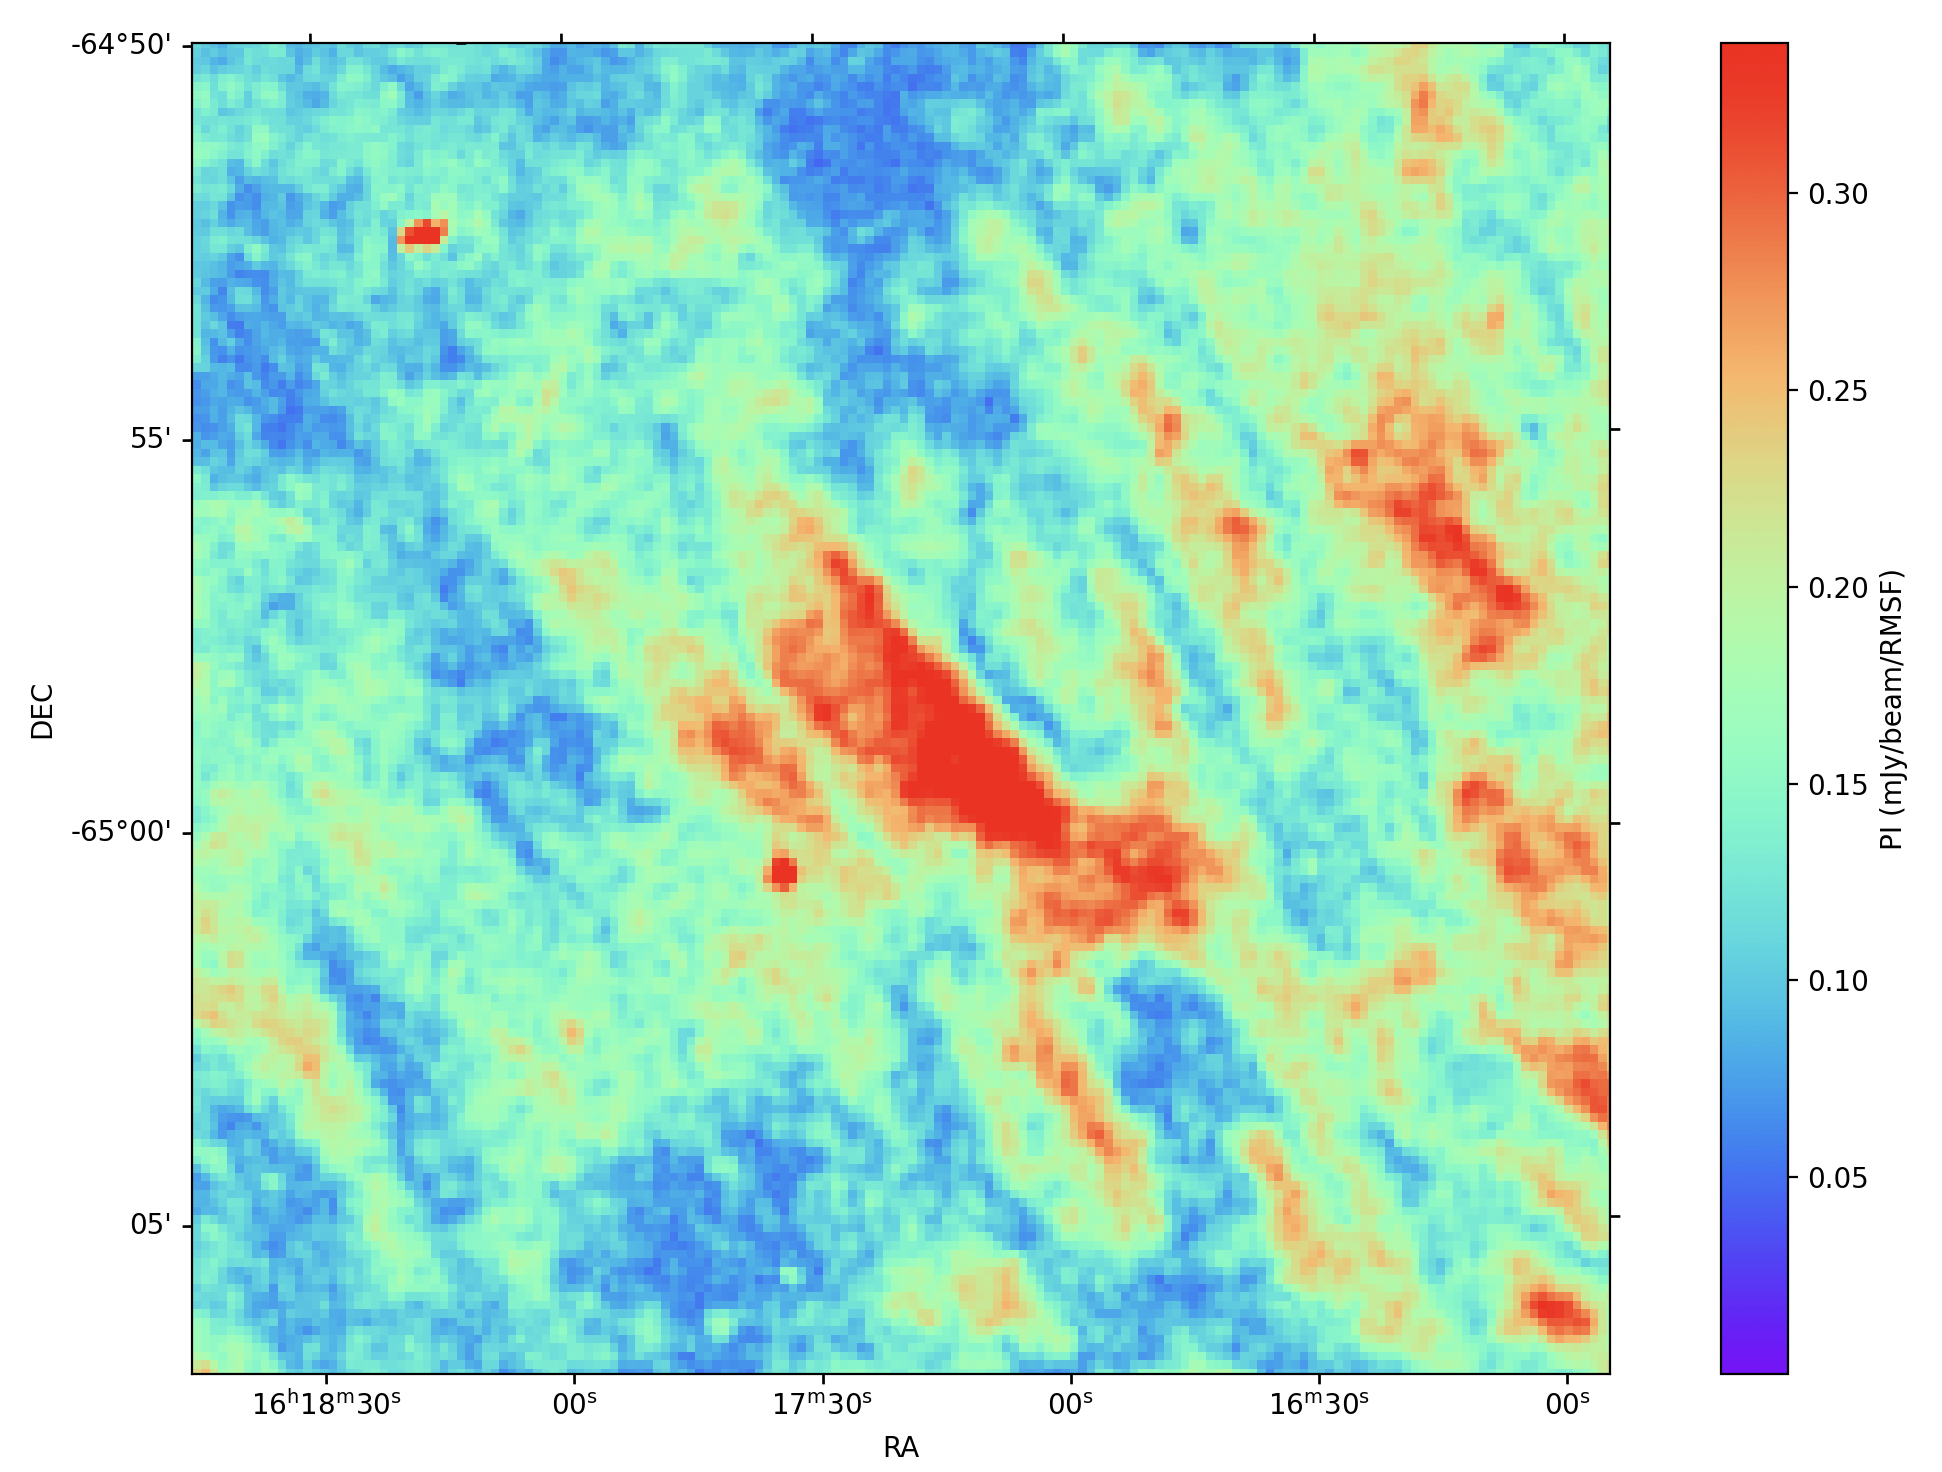
\includegraphics[width=\linewidth]{Thesis_Template/Figures/1615_pi_zoom.png}
        \caption{Zoom in of PI map for field EMU1615-64, with a canal-like feature with a lower PI compared to its surroundings.}
        \label{fig: 1615 pi zoom}
    \end{subfigure}
    \begin{subfigure}[b]{0.6\textwidth}
        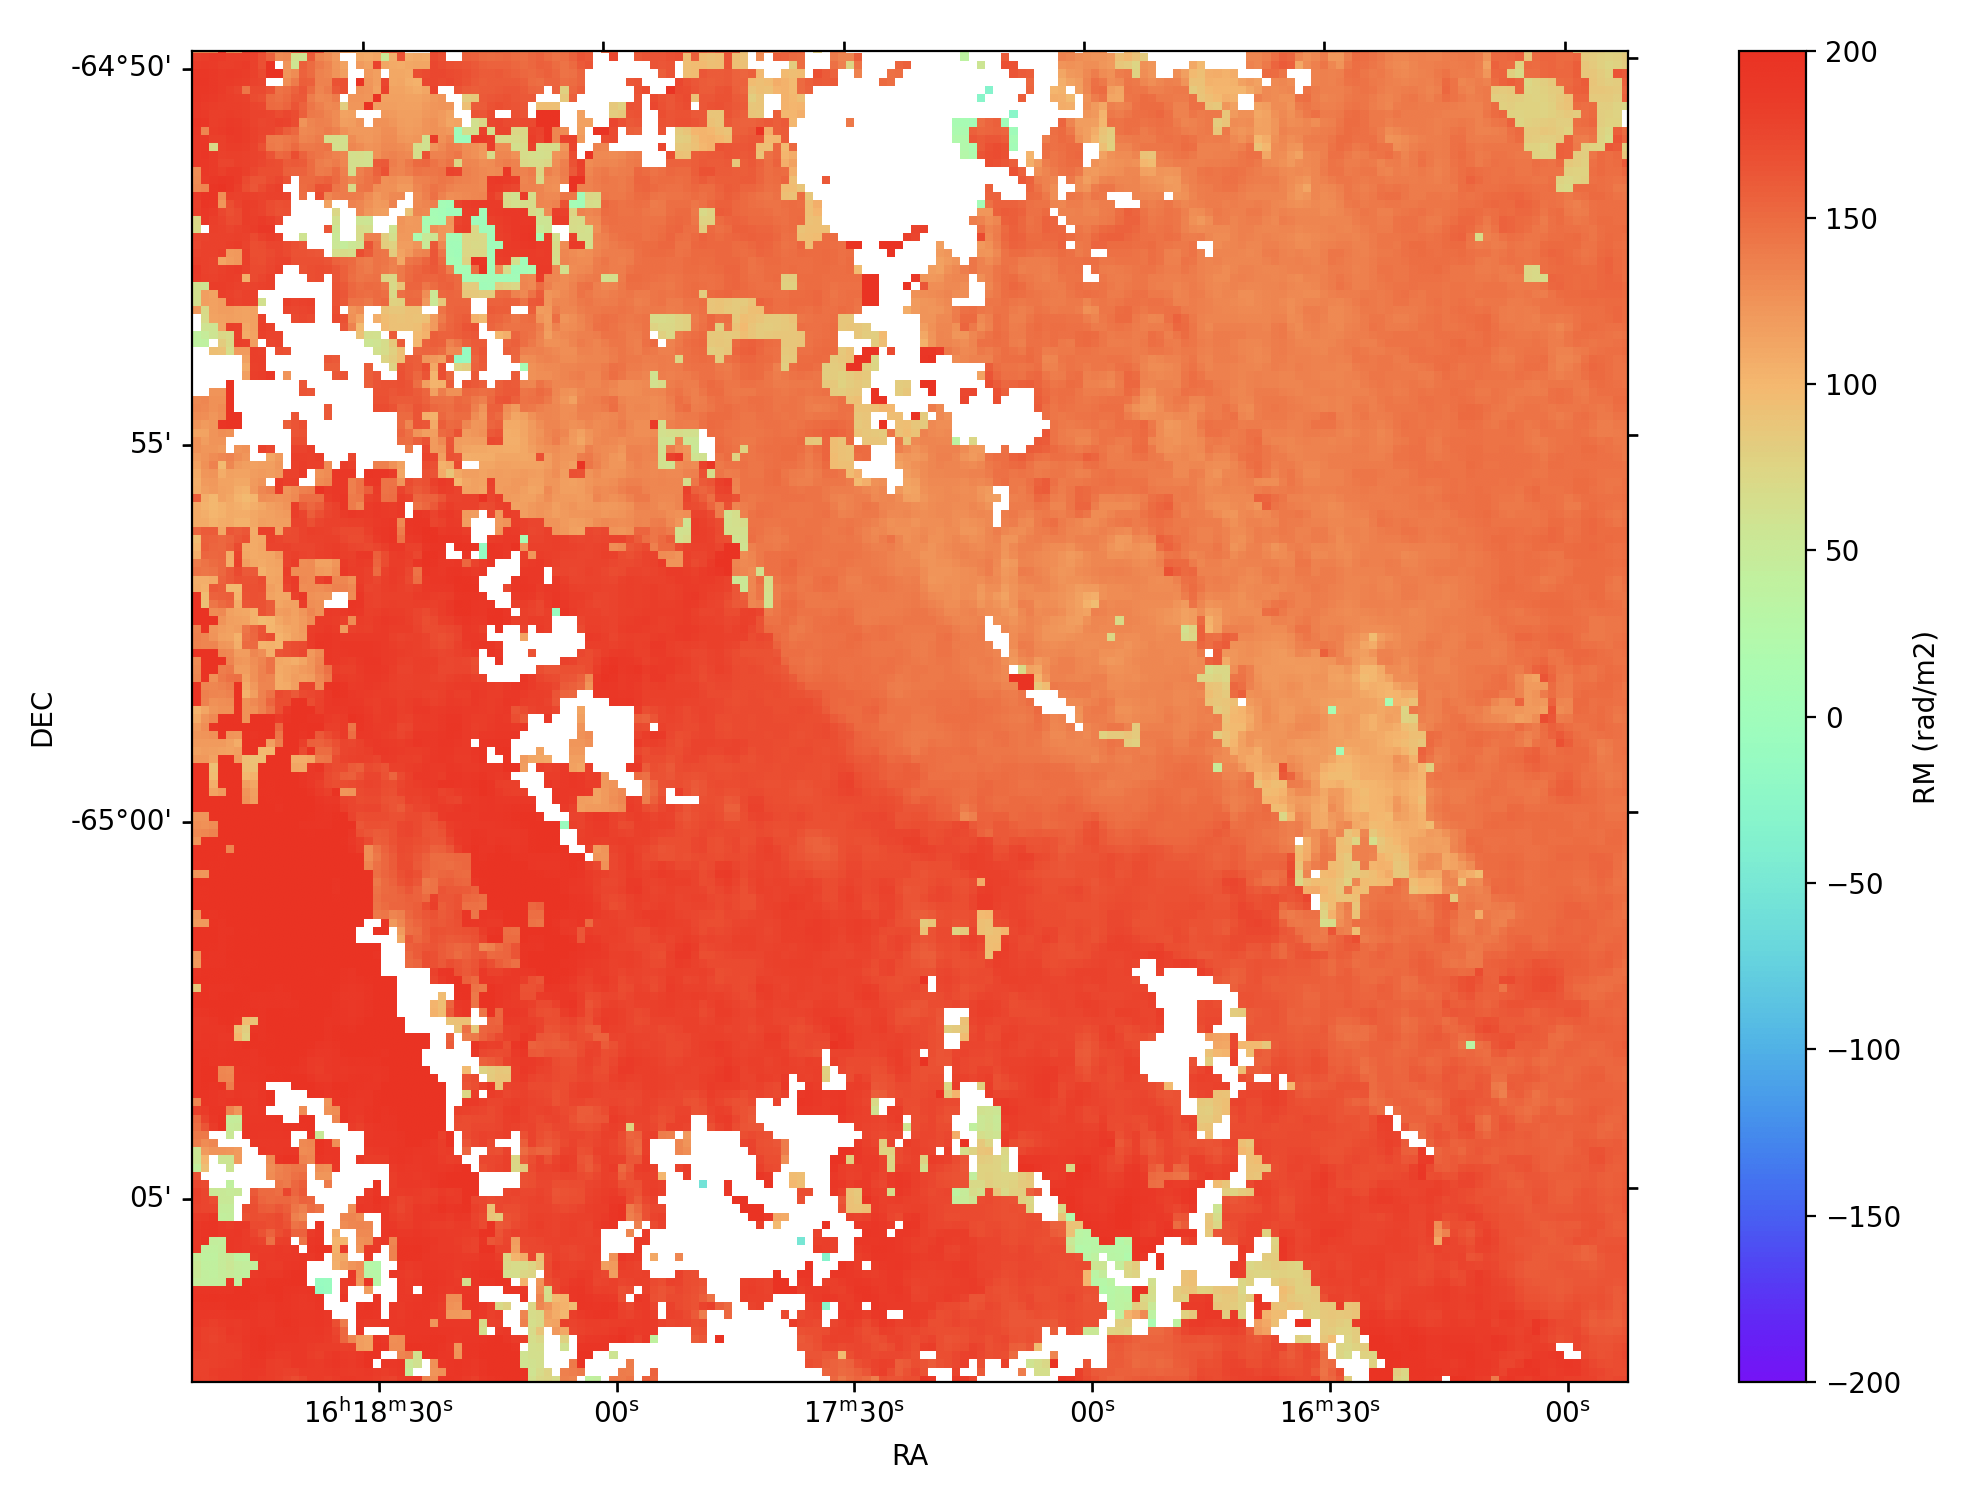
\includegraphics[width=\linewidth]{Thesis_Template/Figures/1615_RM_zoom.png}
        \caption{Zoom in of RM map for field EMU1615-64, showcasing the line of change in RM running across the centre of the image.}
        \label{fig: 1615 rm zoom}
    \end{subfigure}
    \begin{subfigure}[b]{0.7\textwidth}
        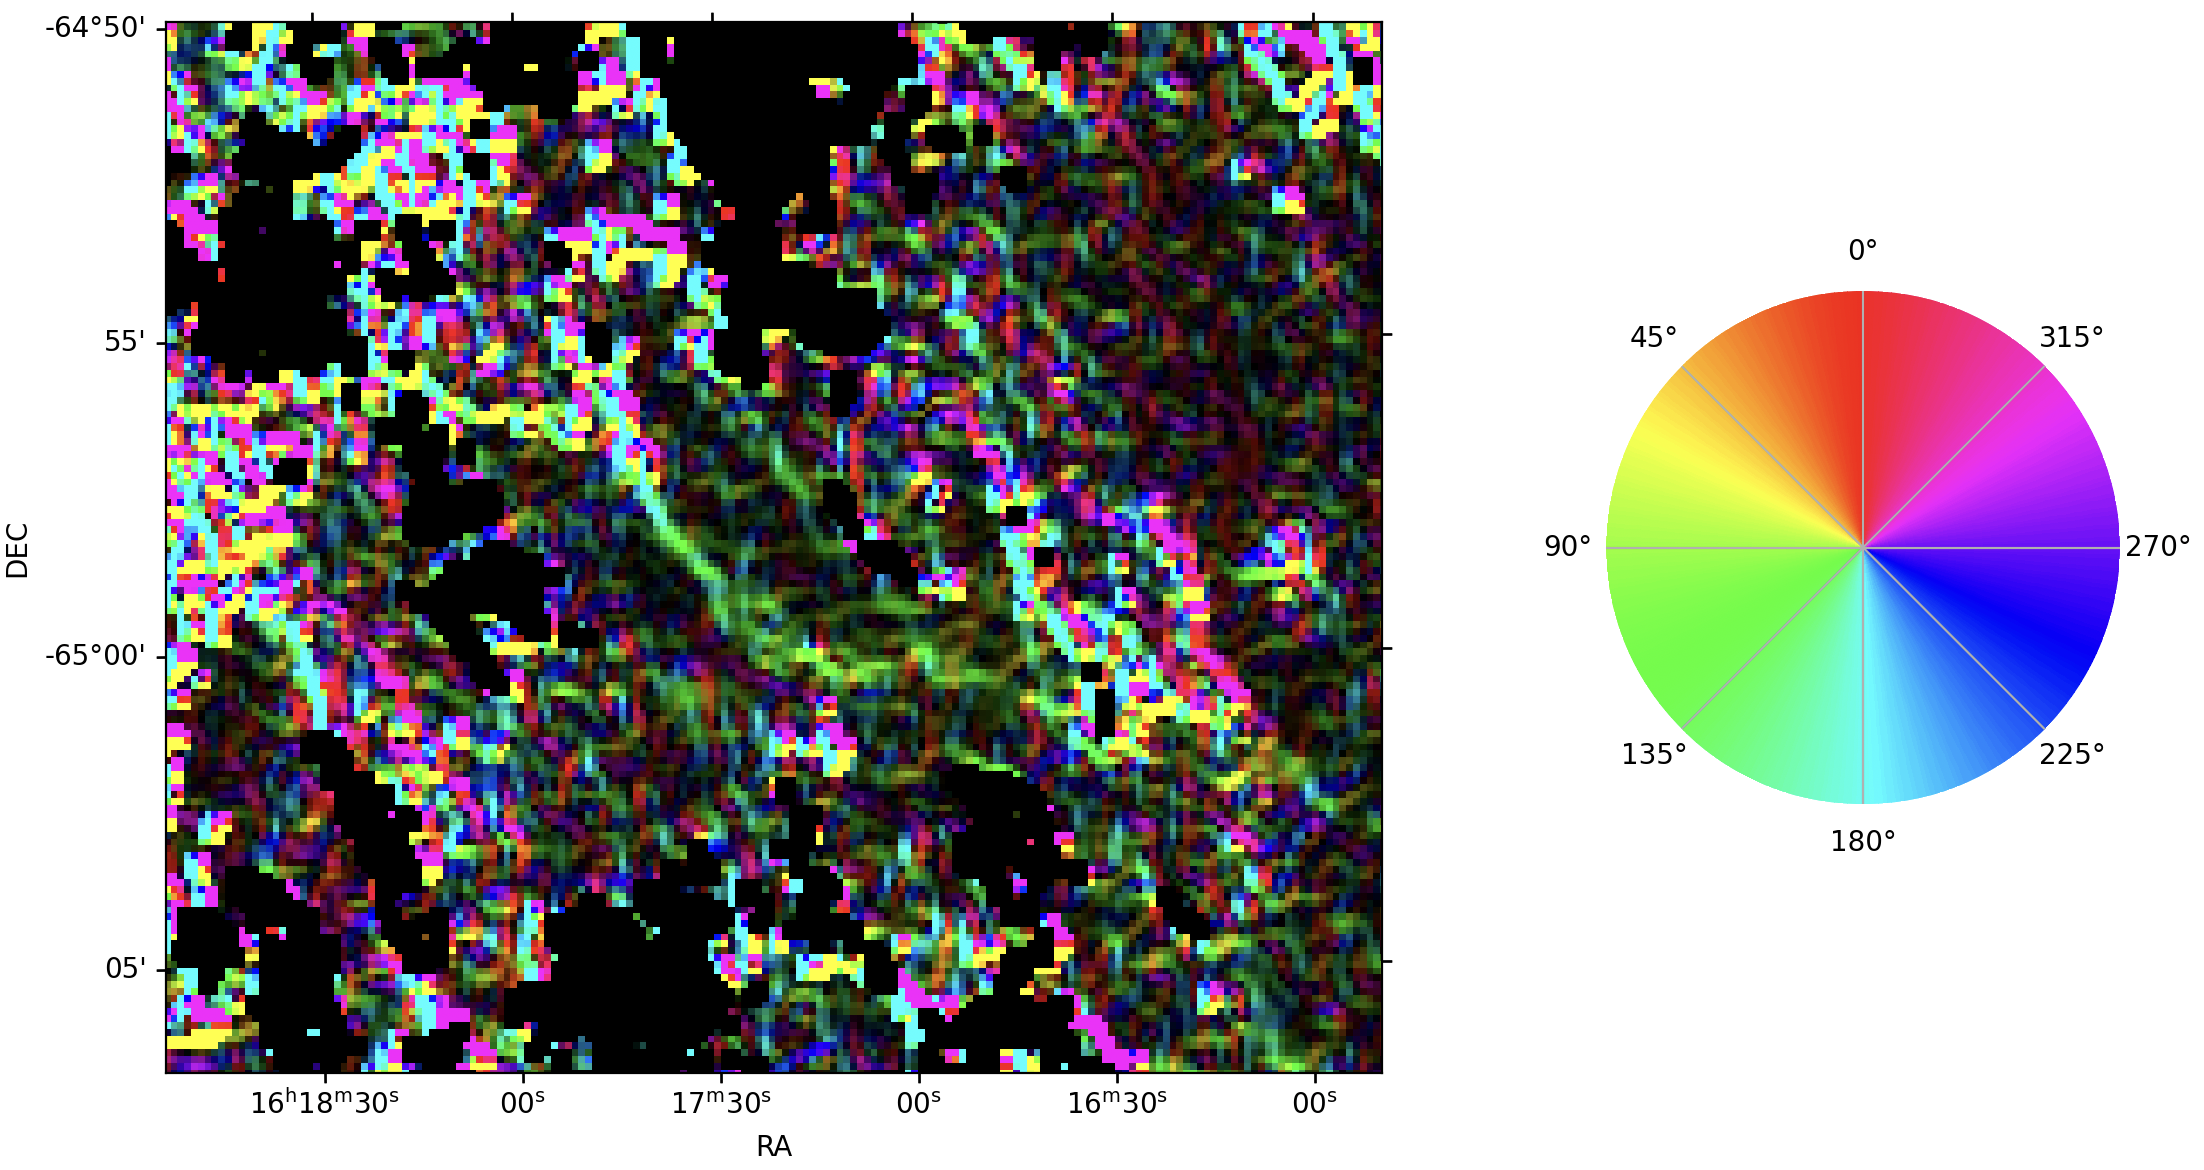
\includegraphics[width=\linewidth]{Thesis_Template/Figures/1615_grad_zoom.png}
        \caption{Zoom in of gradient map for field EMU1615-64, highlighting the central green filament showing a change in gradient of $\sim 135^\circ$.}
        \label{fig: 1615 grad zoom}
    \end{subfigure}
    \caption{Zoom in on feature which can be seen in the centre of all three maps.}
    \label{fig: 1615 zoom}
\end{figure}


Although more work needs to be done to begin to find a conclusive explanation for this phenomena and to be able to create simulations that produce the structure of the diffuse polarisation we are seeing, this work demonstrates the detail in which we are now able to probe with data from POSSUM.



%\include{Thesis_Template/Chapters/Discussion} 
\chapter{Summary and Conclusions}
\label{ch: Conclusion}

I have first outlined the steps of the method used to increase the density of Faraday Rotation measure within the Galactic plane. To do this I first increased the number of sources detected within the Galactic plane by reducing the apparent brightness of the diffuse emission in this region which was being interpreted as noise by applied a second derivative mask to the image. I then used the source finding algorithm PyBDSF to generate a catalogue of sources' positions and brightness. By comparing the positions of sources within a subsection of the image which mainly contained the Galactic plane I concluded that this method successfully increased the number of sources and source density along the Galactic plane by 200$\%$, however this was not as much an improvement as had been expected. 

The next stage in my work was to find the rotation measure values for each of the sources I had found using PyBDSF. After convolving the Stokes cubes to a consistent beam size across all frequency channels and creating a noise profile for each channel, I used the one dimensional POSSUM analysis pipeline to perform rotation measure synthesis. This pipeline extracted the spectrum for each source in the source list, transformed it from frequency to Faraday space and fit the Faraday depth function. From this the Rotation measure value of these sources was found. In this way, the increased source list allowed for an increase to the density of RM along the Galactic plane. With these RM I then constructed an RM grid to visualise the magnetic field across the image. 

I then performed a structure function analysis on this RM grid to find the average difference in RM given a separation in both position angle and angular separation between two sources. This analysis revealed that sources at all separations have a large difference, approximately 200 rad$\,$m$^{\shortminus2}$, meaning that there is rapid variation of RM across the field. This also gave an insight into what physical scale these variations were happening on, which could be as small as 1$\,$pc. It can be seen that the variations are greater along the Galactic plane, and thus future work finding the structure function of sources purely off or on the Galactic plane would further our understanding of the Galactic plane.

I also used the three dimensional POSSUM analysis pipeline to produce a cube of Faraday depth at each frequency. This pipeline also produced a two dimensional images of the peak RM and polarised intensity for the field. Much like the RM grid, these results indicated that the Galactic magnetic field was rapidly varying. They also showed interesting structure across the image, in particular filament-like depolarisation canals.

In order to check that the structure that could be seen in this maps is in fact the fractional variations in Stokes Q and U, I compared the PI and RM values found across the whole bandwidth and the values found if the RM synthesis process was run on the lowest 100 frequency channels. There was a strong positive correlation between the lower part and the full bandwidth, which means that the diffuse structure is real. 

I then investigated the possibility of multiple peaks in the rotation measure being the cause of the canals by finding each peak within the RM map. Finding the secondary and tertiary peaks within the map did not show significantly different RM values, which suggests that this explanation is not the cause of the depolarisation canals. 

Finally I conducted a gradient analysis on the RM maps for a different POSSUM field that showed significant depolarisation canals. This revealed One thing I didn't do prior to this gradient analysis is clipping of extragalactic sources. This would be a useful step for future work as it would leave a more uniform peak brightness across the field and the gradient changes should be clearer.

The capabilities of ASKAP will allow POSSUM to study and learn about the Galactic magnetic field with detail beyond any previous endeavour, with this dissertation being just a small part working towards the collaboration's aim of creating a RM grid containing one million sources. Similarly, the increased quality of data allows for work on depolarisation canals that has not previously been possible. 

%----------------------------------------------------------------------------------------
%	THESIS CONTENT - APPENDICES
%----------------------------------------------------------------------------------------

\appendix % Cue to tell LaTeX that the following "chapters" are Appendices

% Include the appendices of the thesis as separate files from the Appendices folder
% Uncomment the lines as you write the Appendices

% Appendix B

\chapter{1D Pipeline Output} % Main appendix title
\label{AppB: 1D Pipeline Output}

\begin{center}
\begin{tabular}{||c|p{10cm}||} 
\hline
ra & Right Ascension \\
\hline
dec & Declination \\
\hline
beam major & Major axis of synthesised beam \\
\hline
beam minor & Minor axis of synthesised beam \\
\hline
beam pa & Position angle of synthesised beam \\
\hline
polyOrd & Polynomial order of Stokes I model \\
\hline
Ifitstat & Stokes I model fitting flag \\
\hline
IfitChiSqRed & Stokes I fitting reduced chi squared values \\
\hline
sigmaAddQ & Additional scatter required to explain complexity in Stokes Q spectrum. Normalised to scatter in residual Stokes spectrum\\
\hline
dSigmaAddMinusQ & Negative 1 $\sigma$ uncertainty on marginalised $\sigma_{add,q}$ distribution \\
\hline
dSigmaAddPlusQ & Positive 1 $\sigma$ uncertainty on marginalised $\sigma_{add,q}$ distribution \\
\hline
sigmaAddU & Additional scatter required to explain complexity in Stokes U spectrum. \\
\hline 
dSigmaAddMinusU & Negative 1 $\sigma$ uncertainty on marginalised $\sigma_{add,u}$ distribution \\
\hline
dSigmaAddPlusU & Positive 1 $\sigma$ uncertainty on marginalised $\sigma_{add,u}$ distribution\\
\hline
spectral index & Stokes I model spectral index \\
\hline
spectral index err & Error in Stokes I model spectral index \\
\hline
stokesI & Stokes I model intensity \\
\hline
stokesIerr & Error in Stokes I model intensity \\
\hline
FDF noise empirical & Measured noise in the FDF \\
\hline
rm & Peak Rotation Measure \\
\hline
rm err & Error in peak Rotation measure \\
\hline
polint & Polarised intensity of FDF peak \\
\hline
polint err & Error in polarised intensity of FDF peak \\
\hline
SNR PI & Signal to noise in polarised intensity \\
\hline
stokesU & Stokes U of FDF peak \\
\hline
polangle & In-band polarisation angle of FDF peak \\
\hline
polangle err & Error in in-band polarisation angle of FDF peak \\
\hline

\end{tabular}
\end{center}
\begin{center}
\begin{tabular}{||c|p{10cm}||} 
\hline

derot polangle & Derotated Polarisation angle of FDF peak \\
\hline
derot polangle err & Error in derotated Polarisation angle of FDF peak \\
\hline
reffreq I & Reference frequency for Stokes I \\
\hline
reffreq pol & Reference frequency for polarisation \\
\hline
rmsf fwhm & FWHM of the RMSF \\
\hline
noise chan & Typical noise per channel \\
\hline
FDF noise theoretical & Theoretical noise of FDF \\
\hline
minfreq & Lowest frequency used \\
\hline
maxfreq & Highest frequency used \\
\hline
Nchan & Number of channels used \\
\hline
channelwidth & Typical channel bandwidth \\
\hline
fracpol & Fractional polarisation $p=P_{fit}/I_{\lambda_0}$ \\
\hline



\end{tabular}
\end{center}

% Appendix A



\chapter{3D Pipeline Output} % Main appendix title
\label{AppA: 3D pipeline output}

\begin{center}
\begin{tabular}{||c|p{10cm}||} 
 \hline
snrPIfit & Signal to noise ratio in the fitted polarised intensity. Calculated as the ratio of polarised intensity to theoretical noise without bias correction \\ 
\hline
 polAngle0Fitdeg & Derotated polarisation angle (i.e. angle at point of emission) calculated by subtracting phiPeakPIchanrm2$\times$lamsq0 from polarisation angle \\ 
 \hline
 phiPeakPIfitrm2 & Faraday depth found by fitting the peak \\
 \hline
 peakFDFrealFit & Stokes Q value at the fitted Faraday depth of the peak, calculated by interpolating between adjacent samples \\
 \hline
peakFDFimagFit & Stokes Q value at the fitted Faraday depth of the peak, calculated by interpolating between adjacent samples \\
 \hline
minfreq & Minimum frequency used in RM synthesis \\ 
 \hline
 medianchannelwidths & Typical channel width, calculated by assuming that most channels are adjacent to each other \\
 \hline
 maxfreq & Maximum frequency used in RM synthesis \\
 \hline
 lam0sqm2 & The weighted average of the wavelength squared values of the channels used in the RM synthesis as per \cite{Brentjens_2005}. This minimises polarisation angle swings between samples so all angle in the Faraday depth spectrum correspond to this value of wavelength squared \\
 \hline
 dPolAngle0Fit & error in polAngle0Fit \\
 \hline
 dPhiPeakPIfit & error in peak Faraday depth \\
 \hline
 dFDFcorMAD & Estimated noise in the Faraday depth spectrum, computed using the median deviation from the median (MADFM) of polarised intensity in the spectrum and then correcting to be equivalent to a Gaussian sigma \\
 \hline
 dAmpPeakPIfit & error in polarised intensity equal to dFDFth \\
 \hline
 ampPeakPIfitEff & polarised intensity found by fitting the peak corrected for polarisation bias if snrPIfit > 5. Correction formula is $PI_{eff} = \sqrt{PI^2 - 2.3\times dFDFth^2}$ \\
 \hline
\end{tabular}
\end{center}

%\include{Appendices/AppendixC}

%----------------------------------------------------------------------------------------
%	BIBLIOGRAPHY
%----------------------------------------------------------------------------------------

% \printbibliography[heading=bibintoc]
\label{Bibliography}  % Change the left side page header to "Bibliography"
\bibliographystyle{unsrtnat}  % Use the "unsrtnat" BibTeX style for formatting the Bibliography
\bibliography{Bibliography}

%----------------------------------------------------------------------------------------

\end{document}  
